\pagecolor{CadetBlue!70!green}
\chapter{Erweiterung des Werkzeugkastens: Bauteilkunde}\label{kap:bauteilkunde}

Die folgenden Seiten bieten jeweils eine Einführung in neue Bauteile, für die unterschiedliche Grundlagen aus dem Kapitel \enquote{Bausteine von Algorithmen} benötigt werden. Das Kapitel \enquote{Elektrische Grundlagen} ist zum tieferen Verständnis sicherlich hilfreich, aber für diese vorkonfigurierten Bauteile nicht unbedingt notwendig. Mit den hier vorgestellten Bauteilen lässt sich bereits eine Vielzahl an größeren Projekten umsetzen. Vielleicht hast du eine tolle Idee?

\vspace{3\baselineskip}

\begin{projektueberblick}
	\item Schranke \dotfill \pageref{proj:schranke}
	\item Sekundenzeiger \dotfill \pageref{proj:sekundenzeiger}
	\item Alarmanlage \dotfill \pageref{proj:neigungsalarmanlage}
	\item Automatische Tür \dotfill \pageref{proj:tueroeffner}
	\item Joystick-Motor-Steuerung \dotfill \pageref{proj:joystick-motor}
	\item Fernsteuerung v. LED-Streifen \dotfill \pageref{proj:fernsteuerung-lauflicht}
	\item Wetterstation \dotfill \pageref{proj:wetterstation}
	\item Präzises Thermometer \dotfill \pageref{proj:praezisesthermometer}
	\item Automatischer Scheibenwischer \dotfill \pageref{proj:auto-scheibenwischer}
	\item Pulsmesser \dotfill \pageref{proj:pulsmesser}
	\item Einparkhilfe für ein Auto \dotfill \pageref{proj:einparkhilfe}
	\item Katzentür \dotfill \pageref{proj:katzentuer}
\end{projektueberblick}

\setcounter{aufgabennummer}{0}
\setcounter{projektnummer}{0}

\newpage
\nopagecolor
\section{Servo}
\label{sec:servo}

%\marginpar{%
%	\footnotesize%
%	\zurueck 
%	\hyperref[sec:pwm]{Pulsweitenmodulation}
%}
% Tür, die sich öffnet, wenn eine Bewegung registriert wird
\begin{minipage}{0.7\textwidth}
	Ein Servo ist in der Regel ein kleiner Elektromotor zusammen mit einer elektronischen Steuereinheit, die dazu dient, den Motor auf einen bestimmten Winkel einzustellen. Häufig wird beides zusammen als Servomotor bezeichnet. Angewendet werden Servos in vielen Bereichen - zum Beispiel im Modellbau.
\end{minipage}
\hfill
\begin{minipage}{0.28\textwidth}
	\centering
	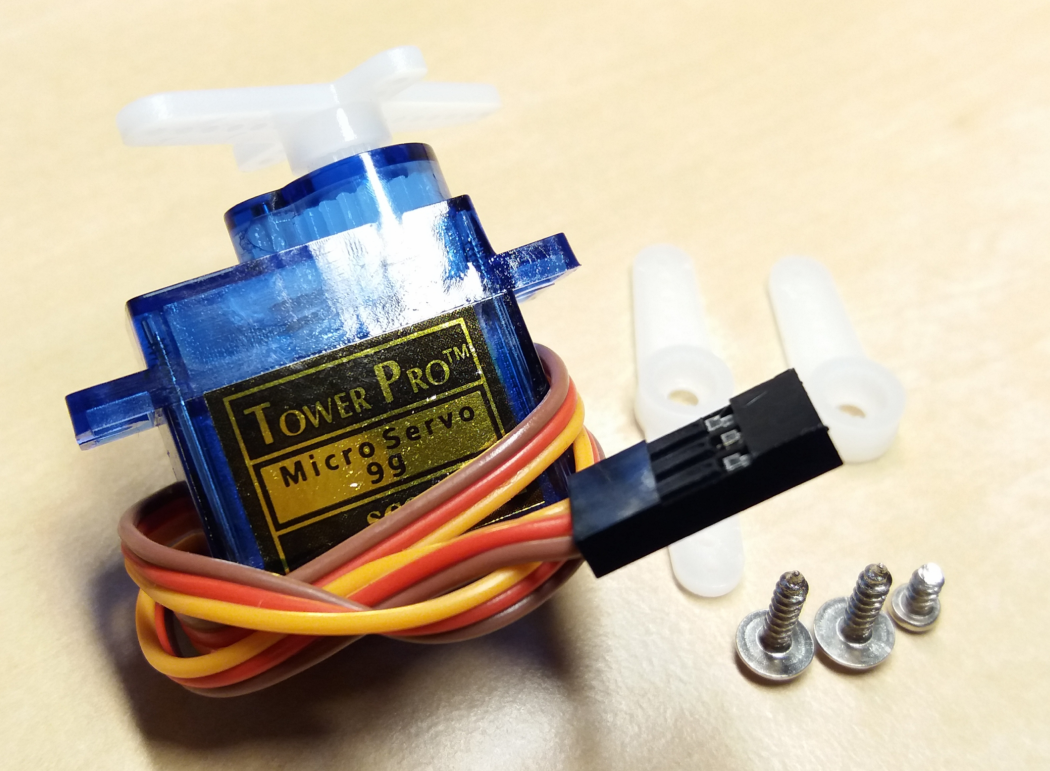
\includegraphics[width=0.9\textwidth]{./pics/servo.png}
\end{minipage}


\begin{figure}[H]
	\centering
	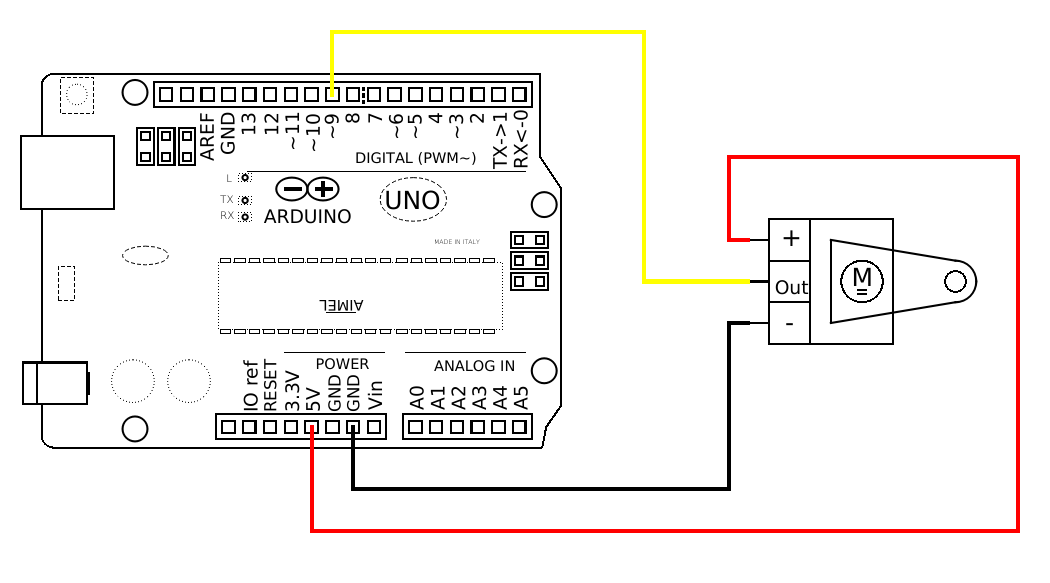
\includegraphics[width=0.7\textwidth]{./Zeichnungen/schaltplan-servo.png}
	\caption{Verschaltung eines Servo am Arduino.}
\end{figure}

Der Servo wird mit drei Anschlüssen an den Arduino angeschlossen:

\begin{itemize}[itemsep=0mm, parsep=0mm]
	\item VCC (rot): Die Stromversorgung des Servo wird mit dem 5\,V-Pin des Arduino verbunden. Dabei ist zu beachten, dass ein Servomotor relativ große Stromstärken \enquote{ziehen} kann. Der 5\,V-Pin des Arduino kann bis zu $\SI{200}{\milli\ampere}$ ausgeben, bevor er durchbrennt. Das ist für den Servo genug. Ein normaler Digitalpin verträgt dagegen nur $\SI{40}{\milli\ampere}$, was deutlich zu wenig für den Servo ist. Die Stromversorgung des Servo kann also nicht über einen normalen Digitalpin sichergestellt werden.
	\item GND (schwarz/braun): Die Stromversorgung ist nur komplett, wenn auch das GND-Niveau auf das GND-Niveau des Arduino festgelegt wird.
	\item Signalleitung (gelb): Die Einstellung des Winkels erfolgt über ein Pulsweitenmodulation, allerdings wird diese von einer zusätzlichen Bibliothek bereitgestellt, sodass das gelbe Kabel mit jedem Digitalpin am Arduino verbunden werden kann.
\end{itemize}

\medskip
\begin{projekt}[Schranke]\label{proj:schranke}
	\begin{minipage}{0.6\textwidth}
		Baue mit einem Servo eine Schranke, die auf Knopfdruck geöffnet und wieder geschlossen werden kann.		
	\end{minipage}
	\hfill
	\begin{minipage}{0.38\textwidth}
		\vspace{-\baselineskip}
		\begin{figure}[H]
			\centering
			
\includegraphics[width=\textwidth]{./pics/servo-steuerung.png}
			\caption{Die Servo-Steuerung erfolgt über Angabe eines Winkels zwischen $\ang{0}$ und $\ang{180}$.}
		\end{figure}
	\end{minipage}
\end{projekt}

\begin{recherche}{Wie funktioniert die Steuerung eines Servos?}
	Der Winkel, auf den sich die Ausgangswelle des Servo drehen soll, wird über ein PWM-Signal geregelt. Recherchiere im Internet, wie dies realisiert wird und fasse es zusammen.
\end{recherche}

\newpage
\section{Schrittmotor}\label{sec:schrittmotor}

%\begin{minipage}{0.7\textwidth}
%	Während ein Servo darauf ausgelegt ist, einen Winkel möglichst präzise anzusteuern, dient ein Schrittmotor dazu, möglichst präzise Drehungen zu realisieren. Damit können zum Beispiel 3D-Drucker oder Roboterarme, aber auch DVD-Laufwerke sehr genau gesteuert werden.
%\end{minipage}
%\hfill
%\begin{minipage}{0.28\textwidth}
%	\centering
%	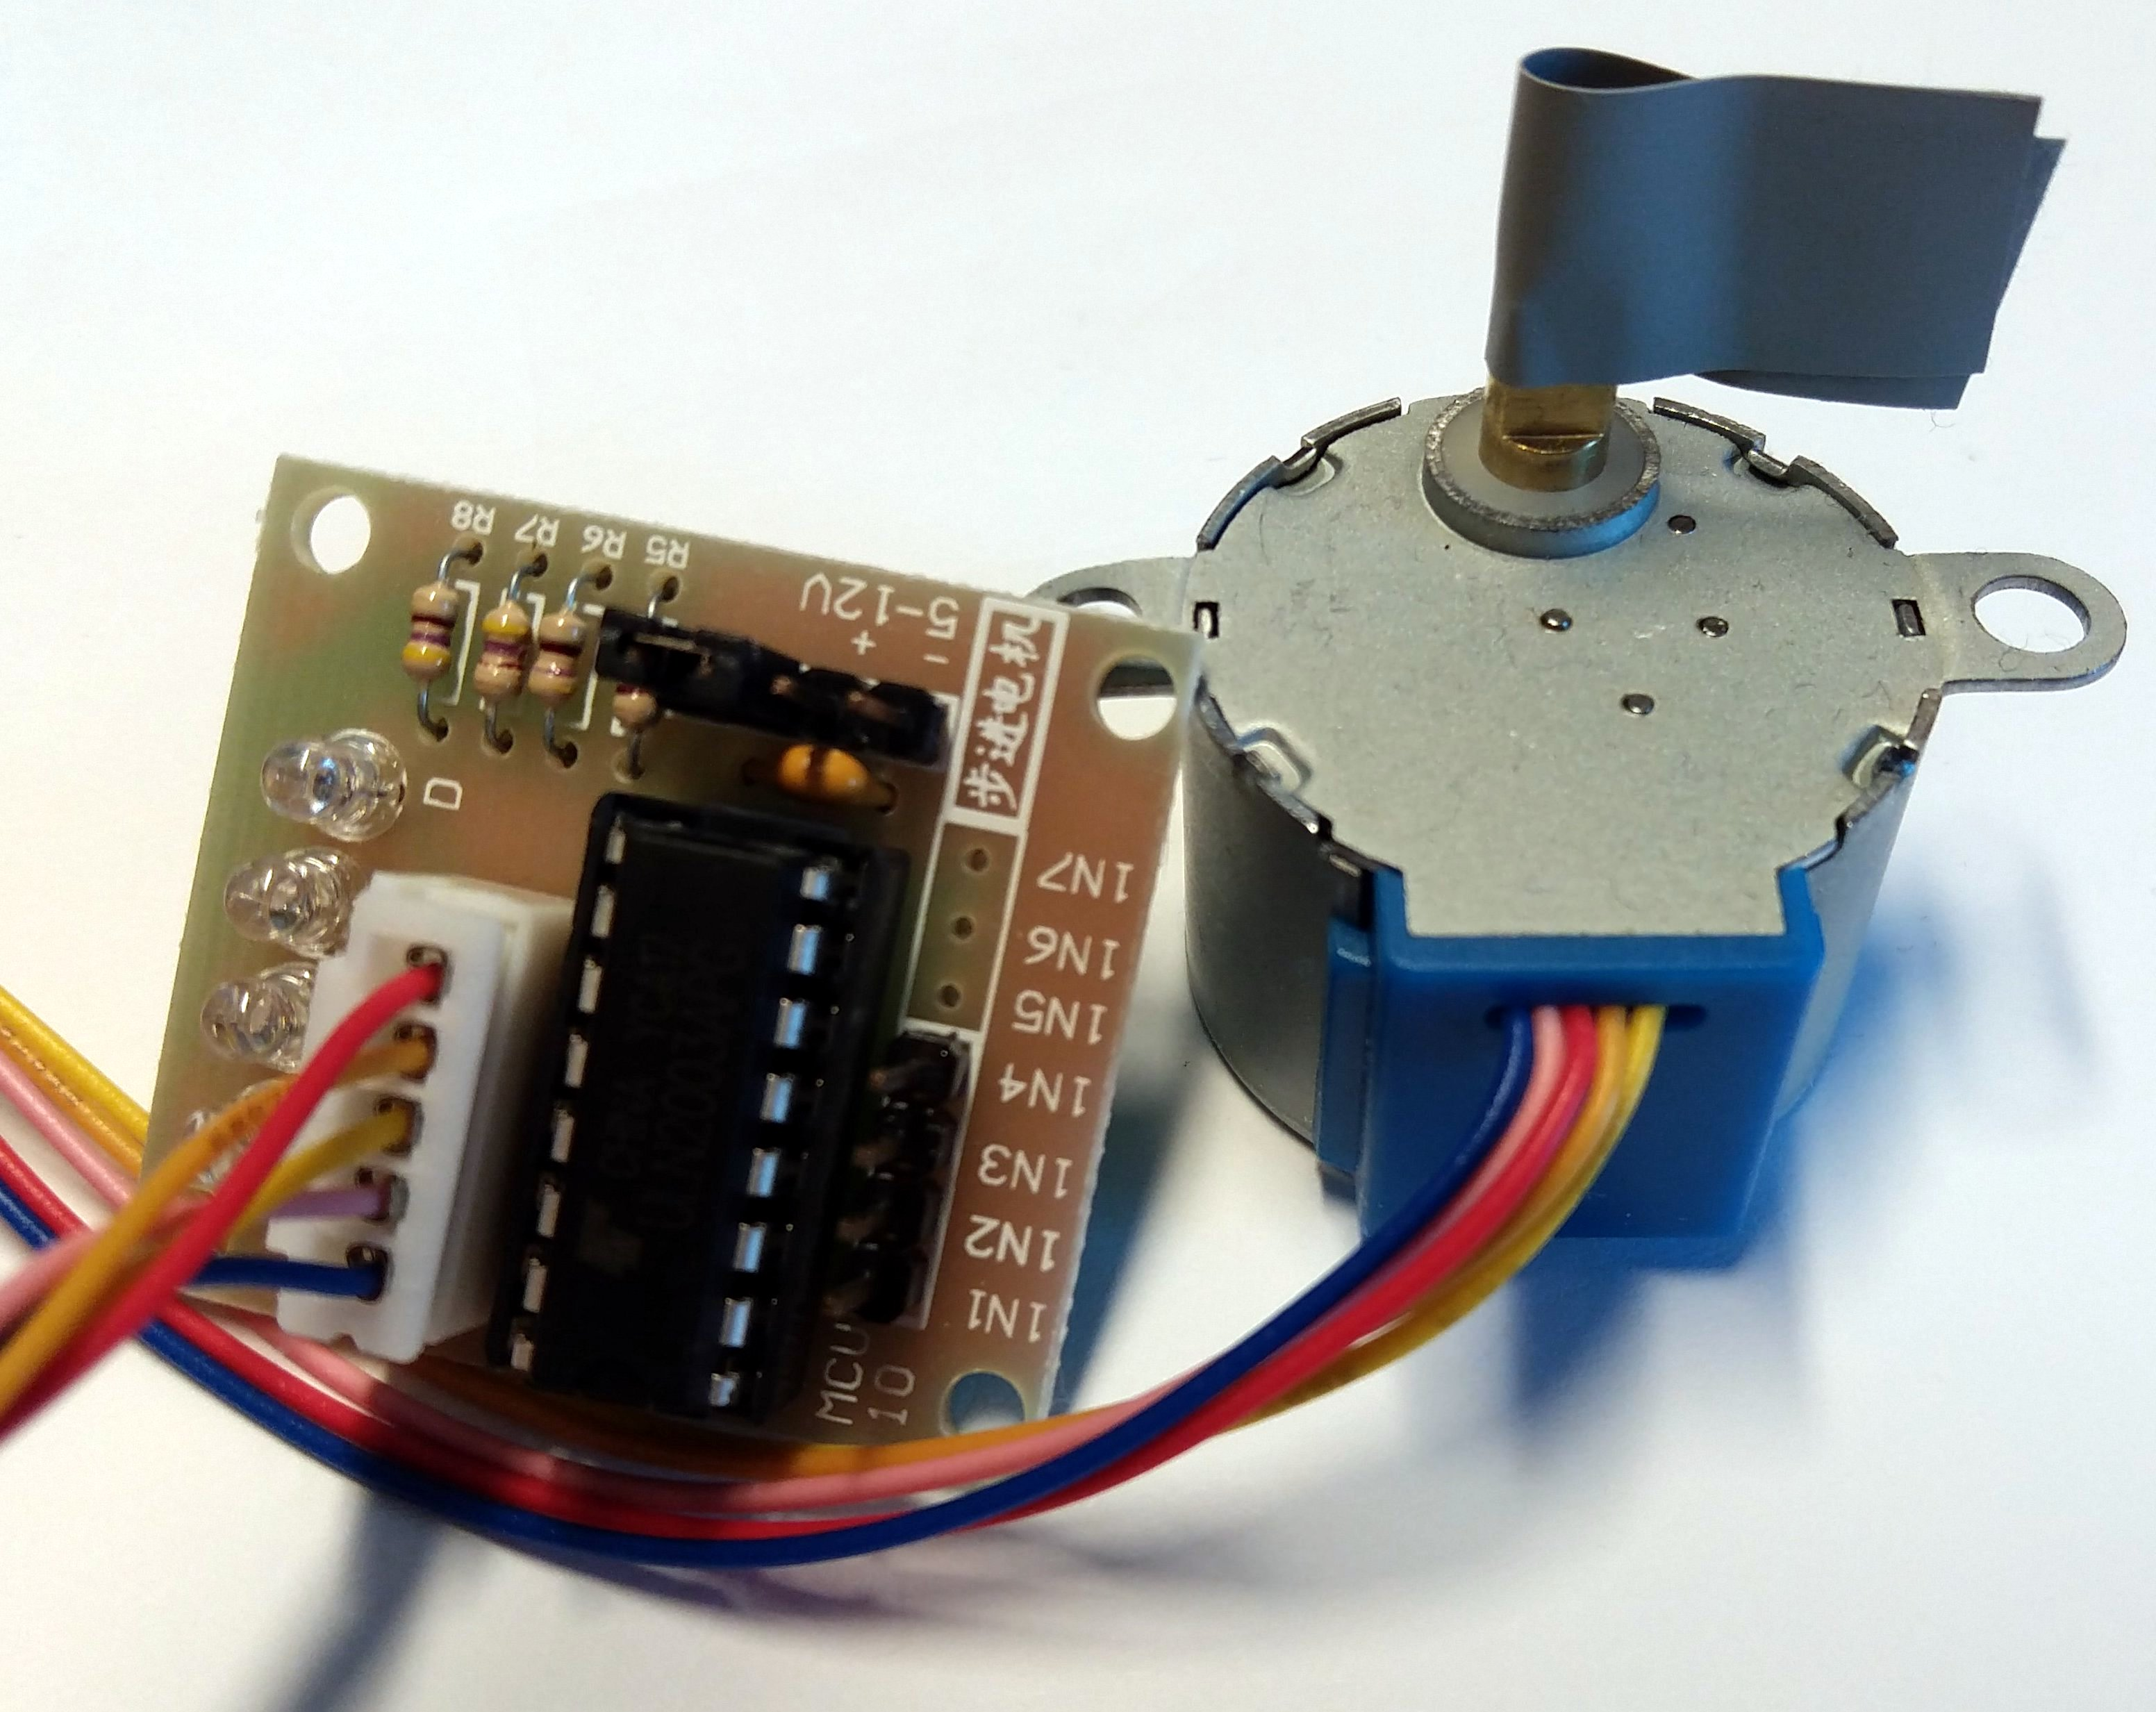
\includegraphics[width=0.9\textwidth]{./pics/schrittmotor.jpg}
%	\caption{Schrittmotor mit Motortreiber ULN2003.}
%\end{minipage}

\begin{wrapfigure}{r}{0.28\textwidth}
	\centering
	\vspace{-0.5\baselineskip}
	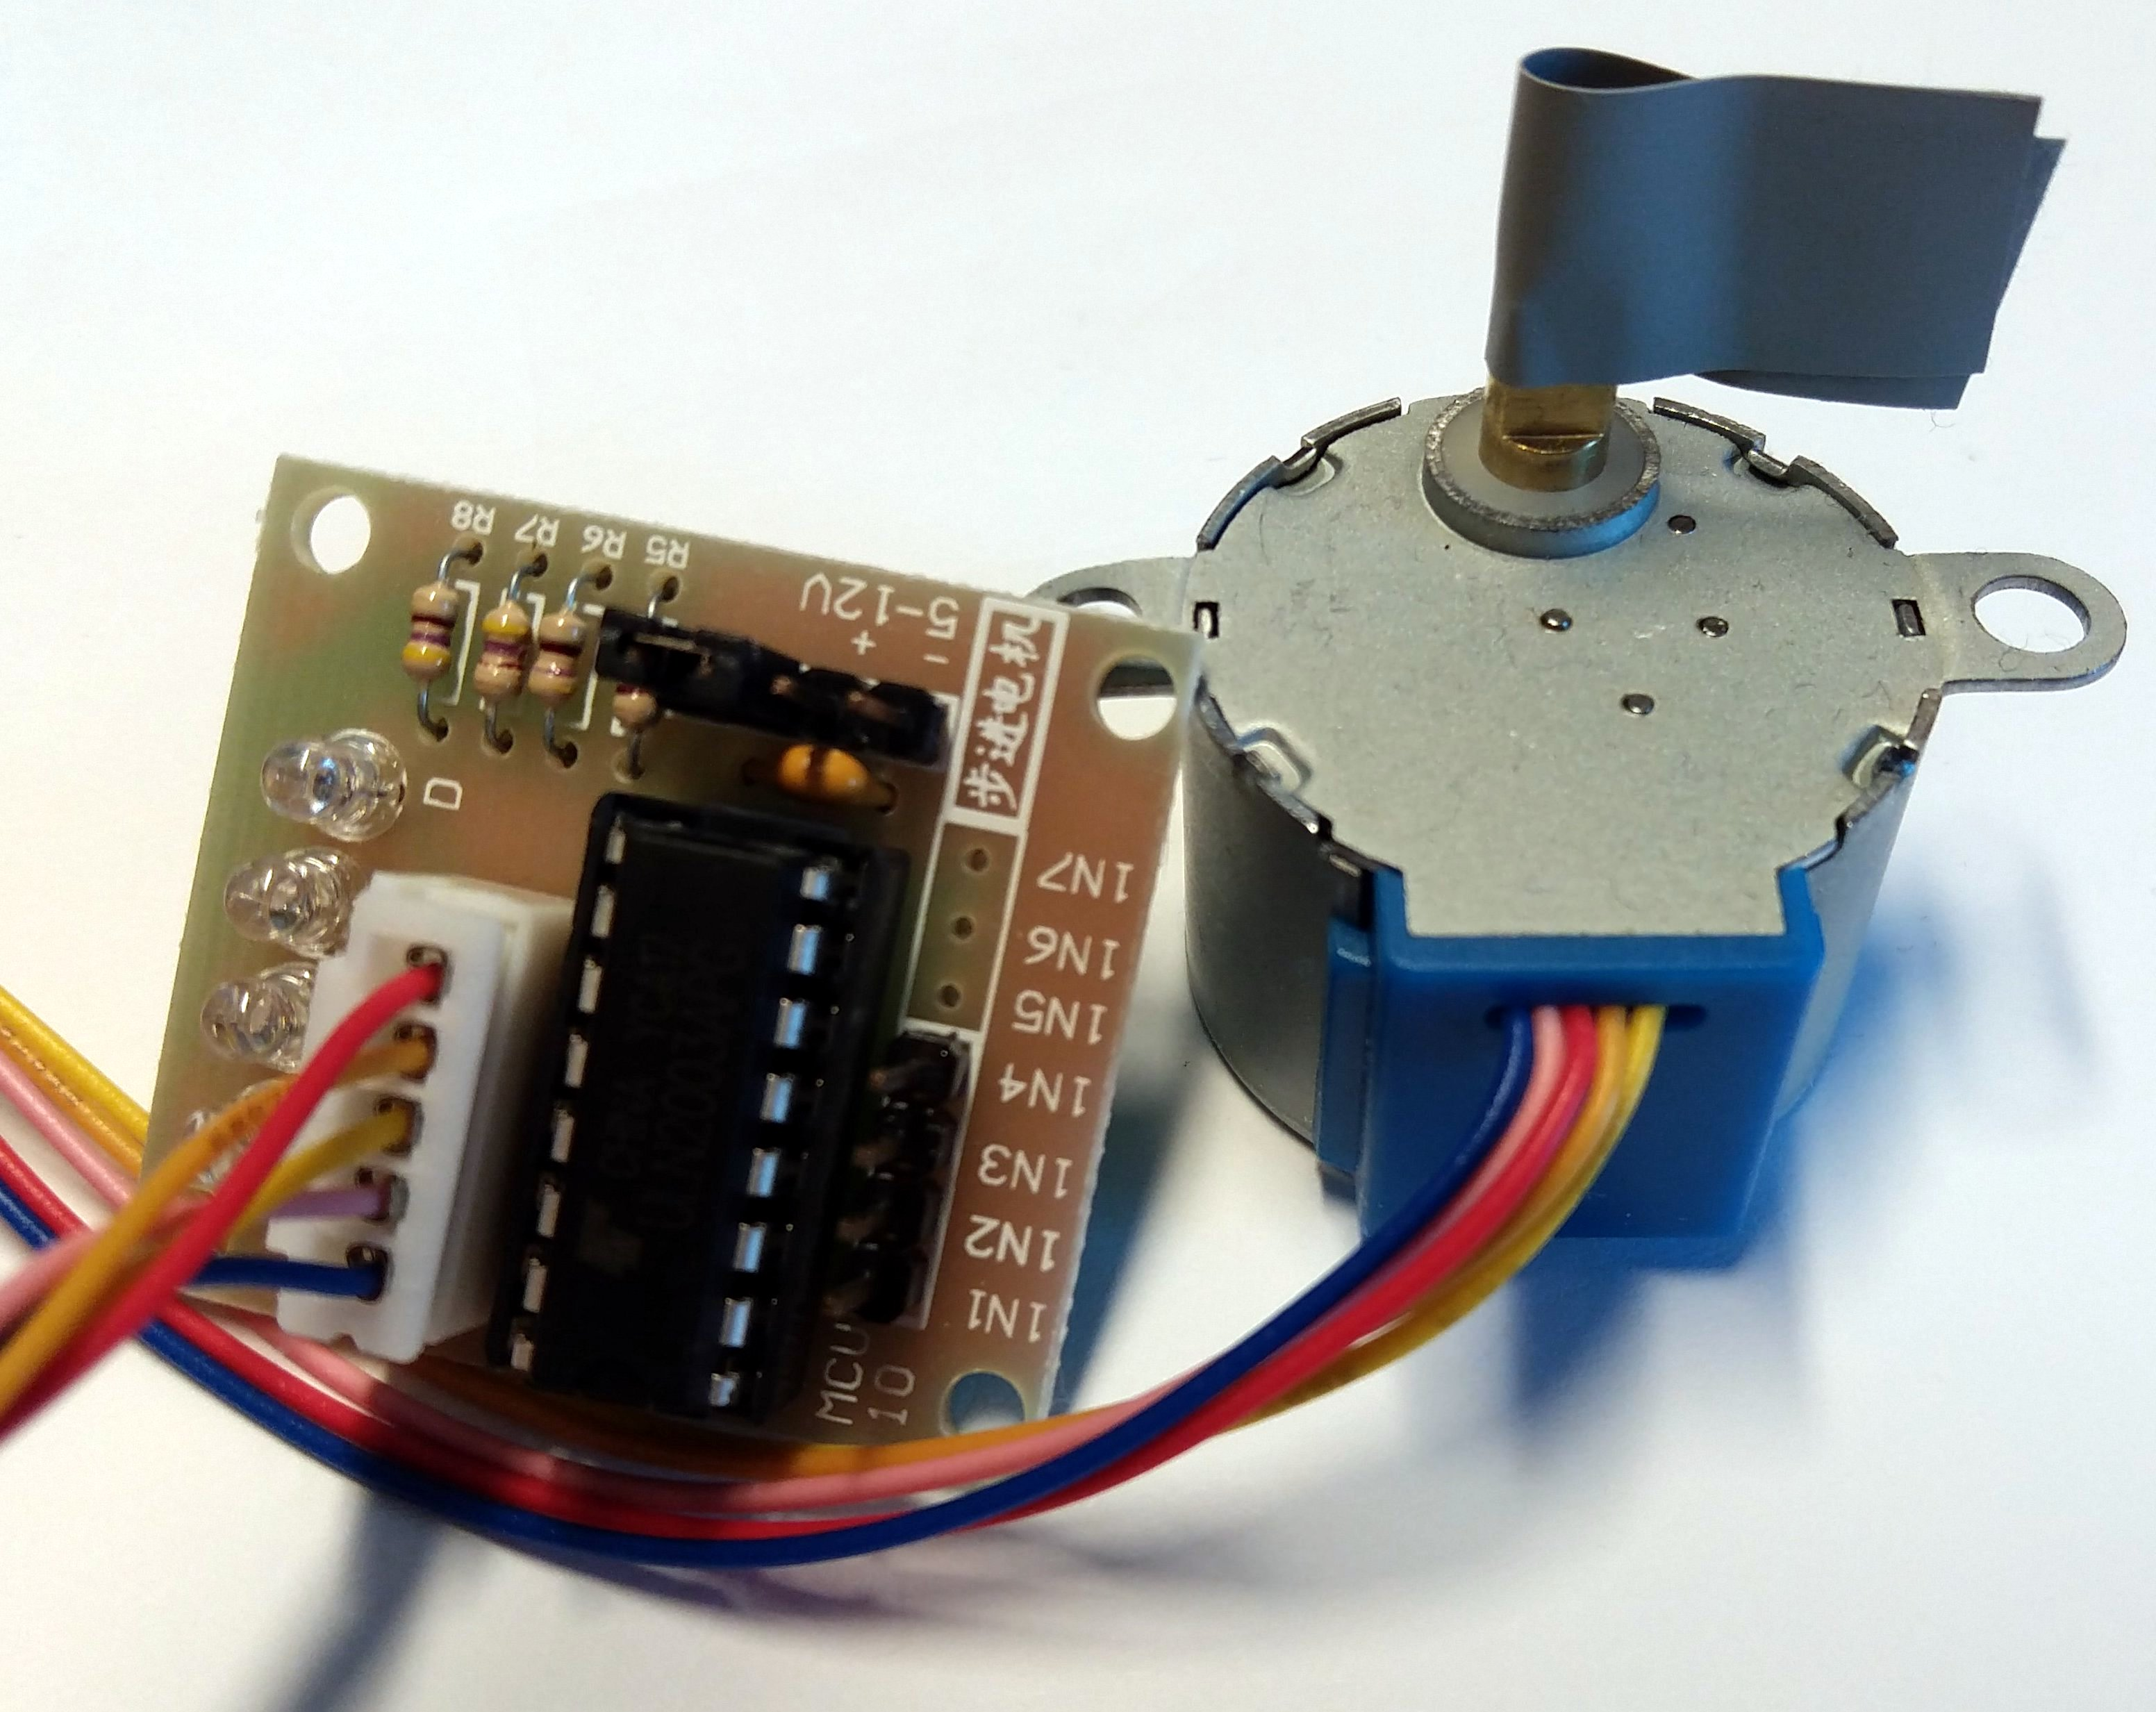
\includegraphics[width=0.252\textwidth]{./pics/schrittmotor.jpg}
	\caption{Schrittmotor mit Motortreiber ULN2003.}
%	\vspace{-\baselineskip}
\end{wrapfigure}
Während ein Servo darauf ausgelegt ist, einen Winkel möglichst präzise anzusteuern, dient ein Schrittmotor dazu, möglichst präzise Drehungen zu realisieren. Damit können zum Beispiel 3D-Drucker oder Roboterarme, aber auch DVD-Laufwerke sehr genau gesteuert werden.

Herzstück des Motors sind zwei Spulen, die jeweils in der Mitte durch eine 5\,V-Spannungsversorgung in zwei Teile geteilt werden. Weil der Pol mit dem positiven 5\,V-Potential dadurch festgelegt ist und nicht flexibel an beiden Enden angelegt werden kann, nennt man den Motor auch \emph{unipolaren} Schrittmotor.

\medskip
\begin{minipage}{0.3\textwidth}
	\begin{figure}[H]
		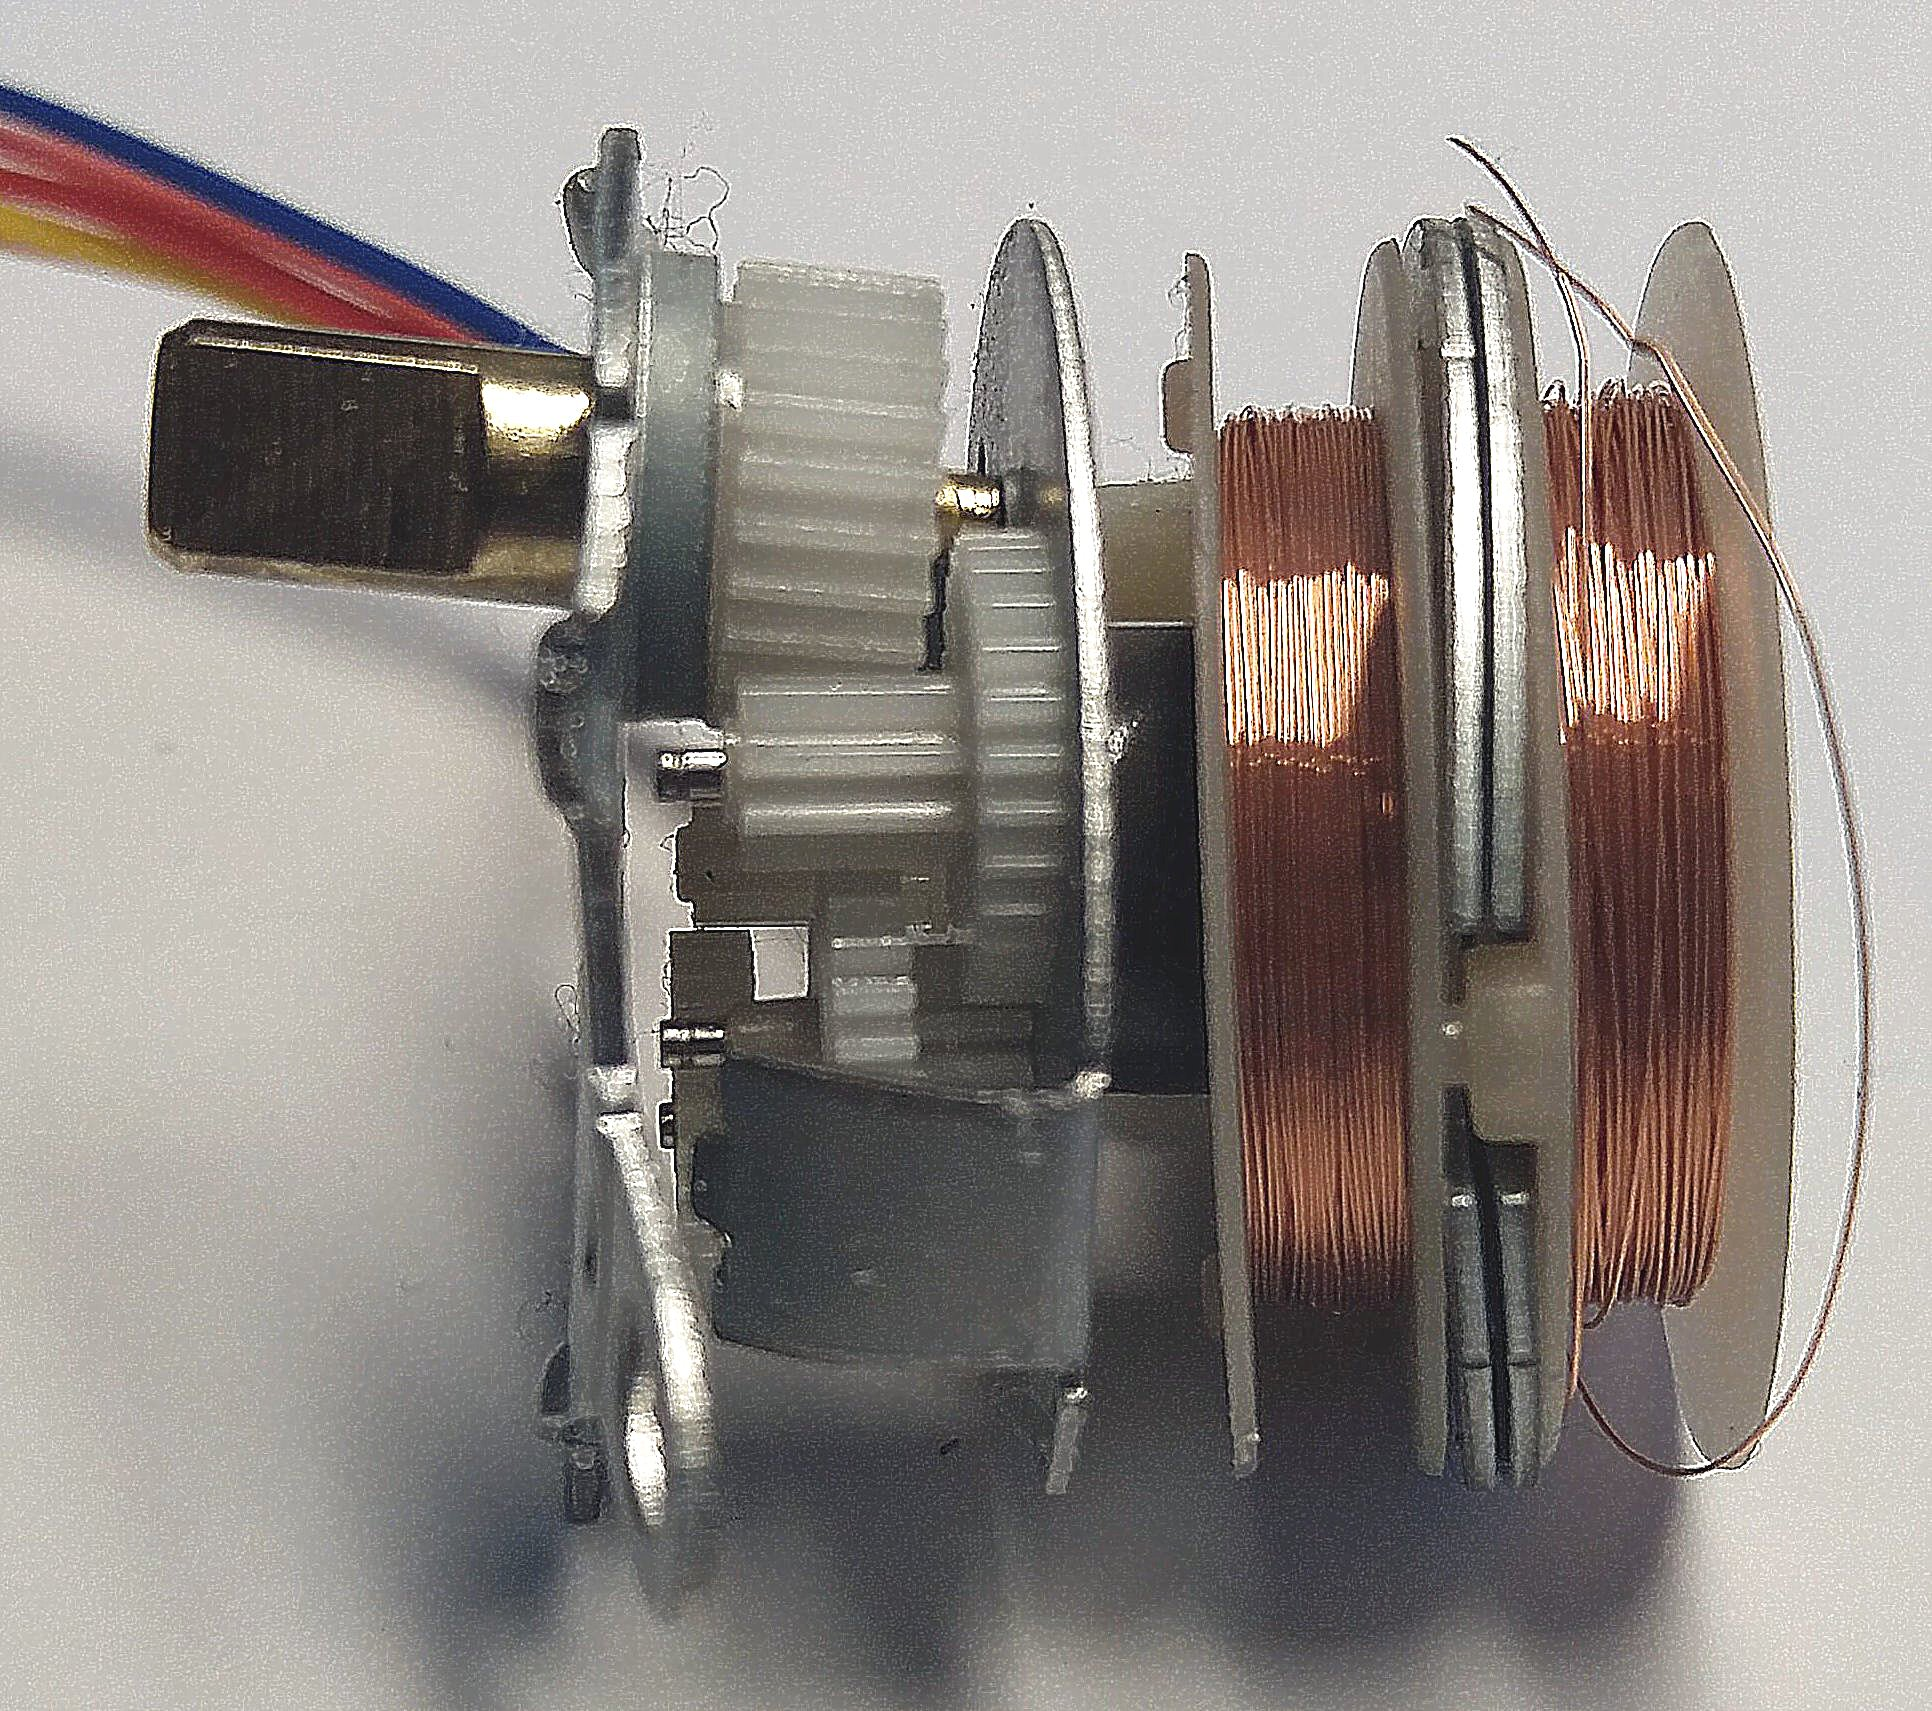
\includegraphics[width=\textwidth]{./pics/schrittmotor-innen.jpg}
		\caption{Innenansicht eines Schrittmotors.}
	\end{figure}
\end{minipage}
\hfill
\begin{minipage}{0.3\textwidth}
	\begin{figure}[H]
		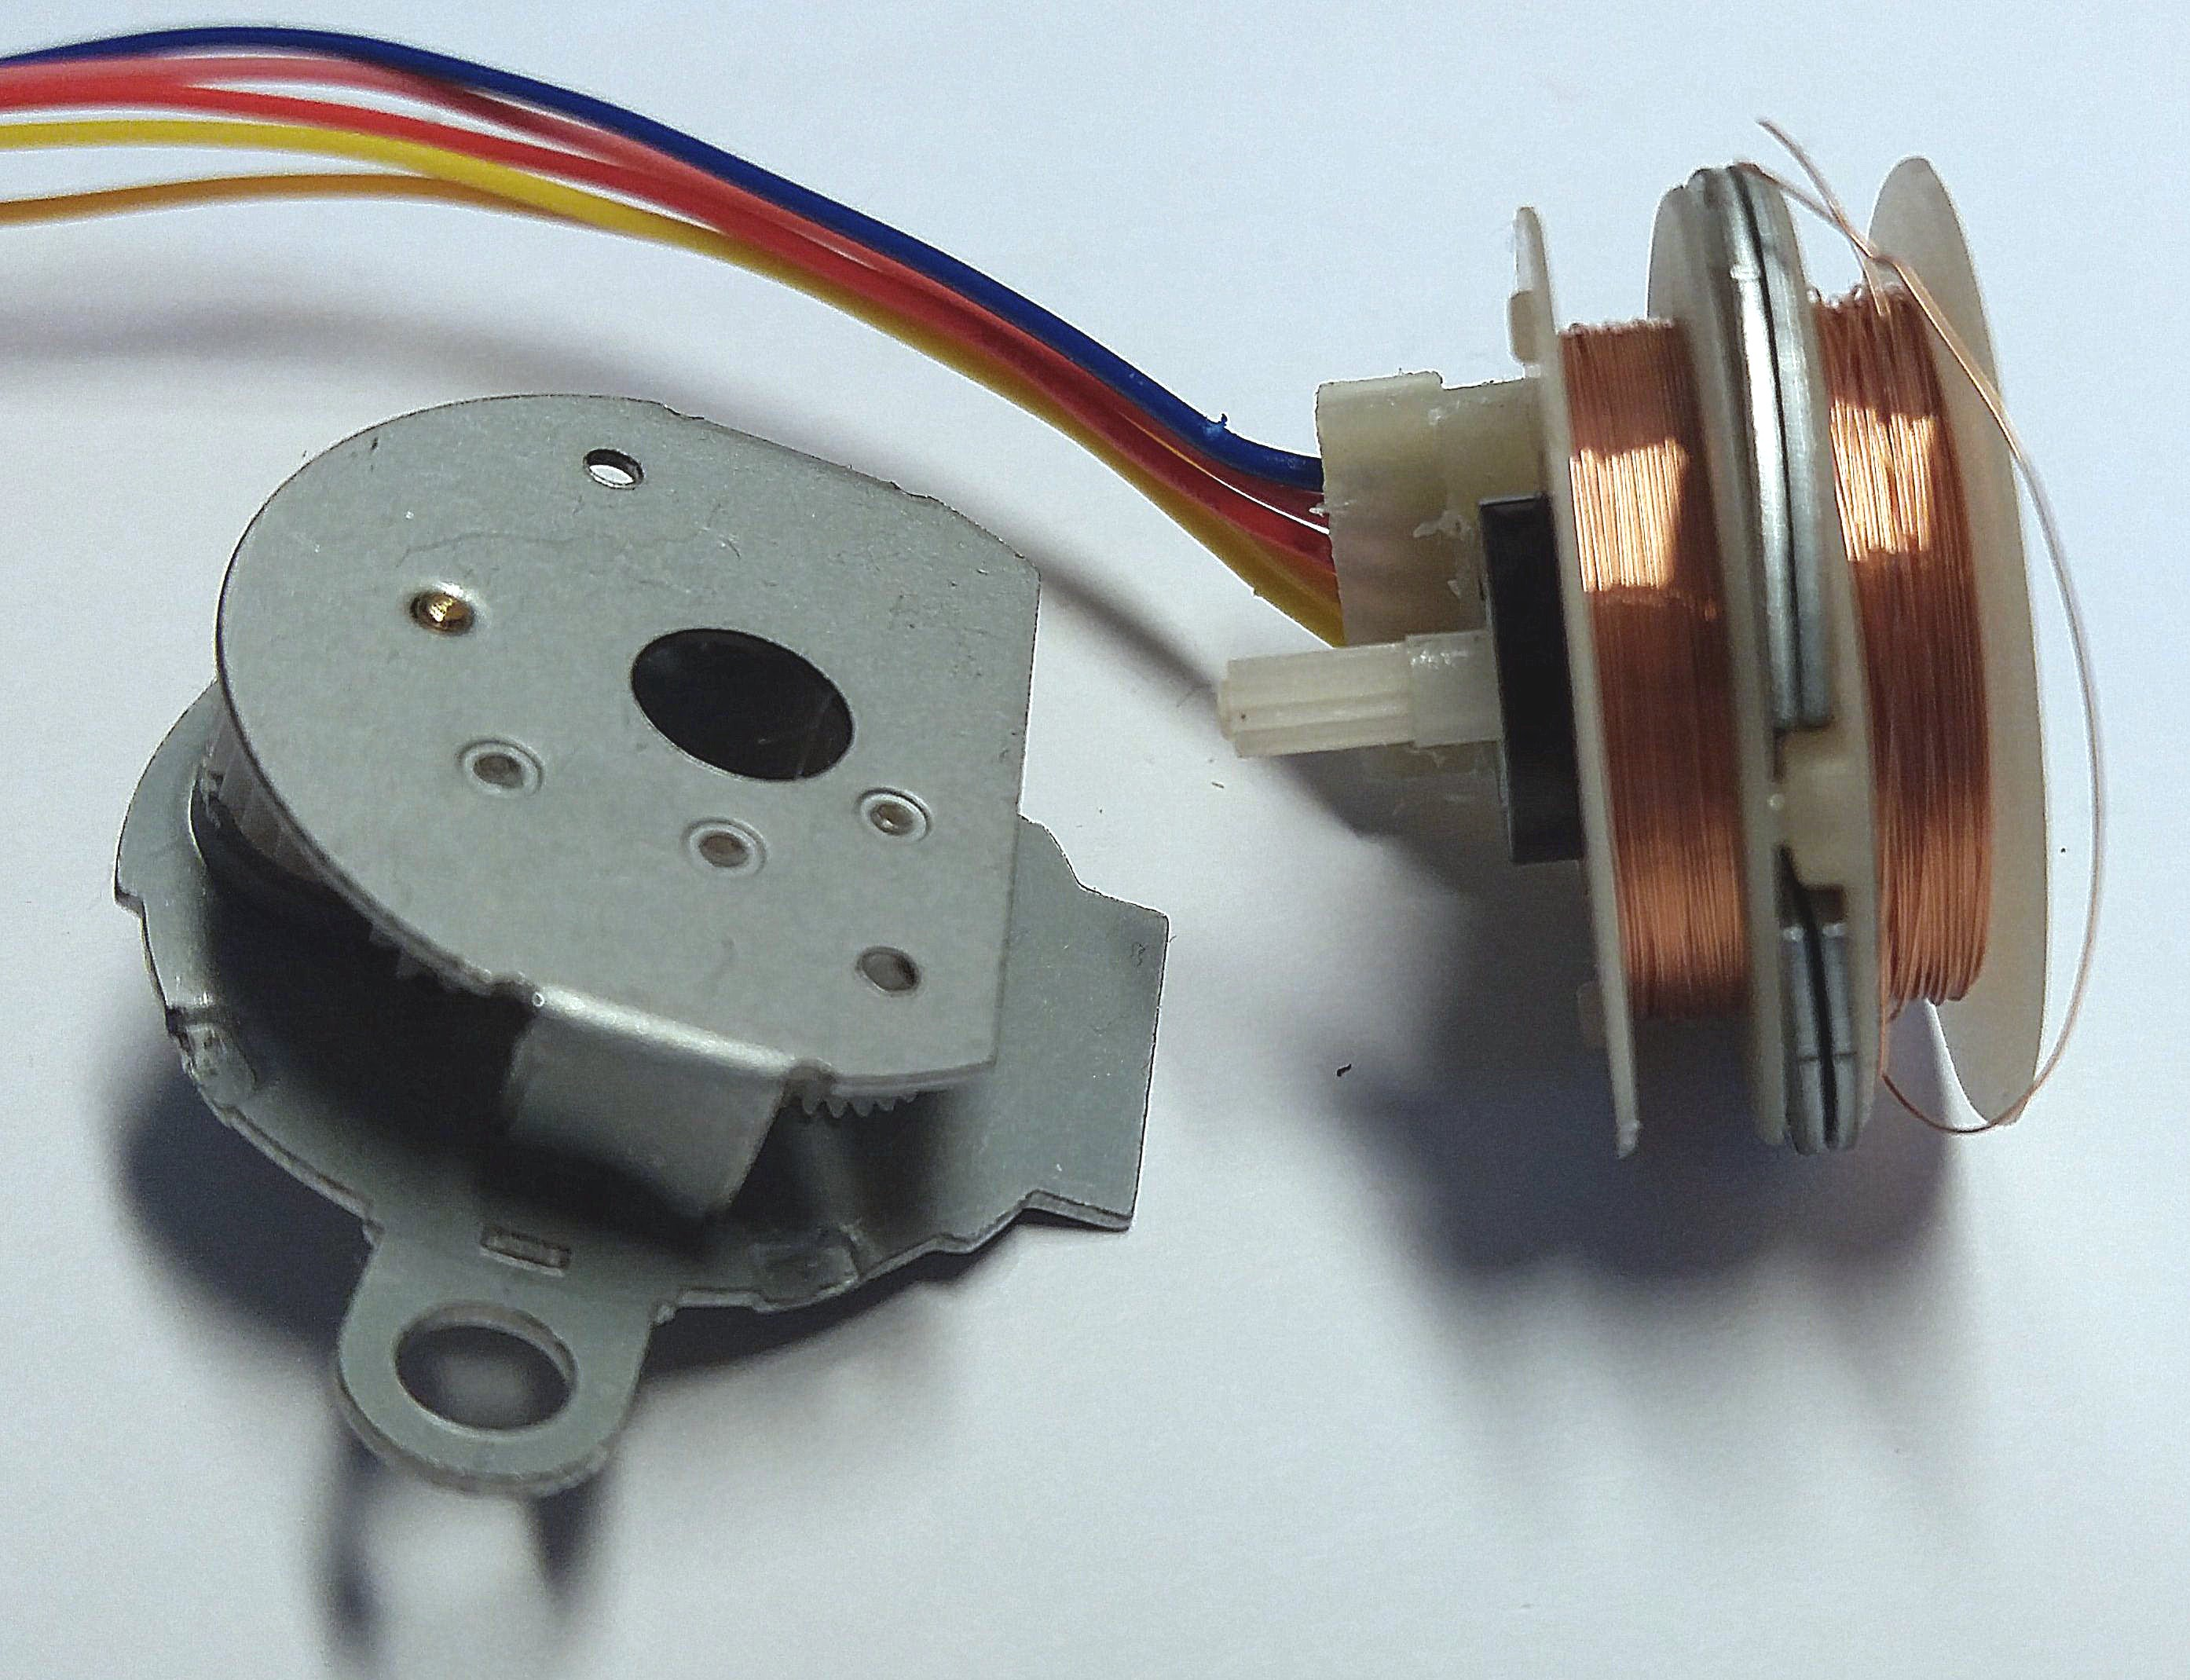
\includegraphics[width=\textwidth]{./pics/schrittmotor-innen-auseinander.jpg}
		\caption{Sicht auf Permanentmagnet mit Zahnrad in den Spulen.}
	\end{figure}
\end{minipage}
\hfill
\begin{minipage}{0.3\textwidth}
	\begin{figure}[H]
		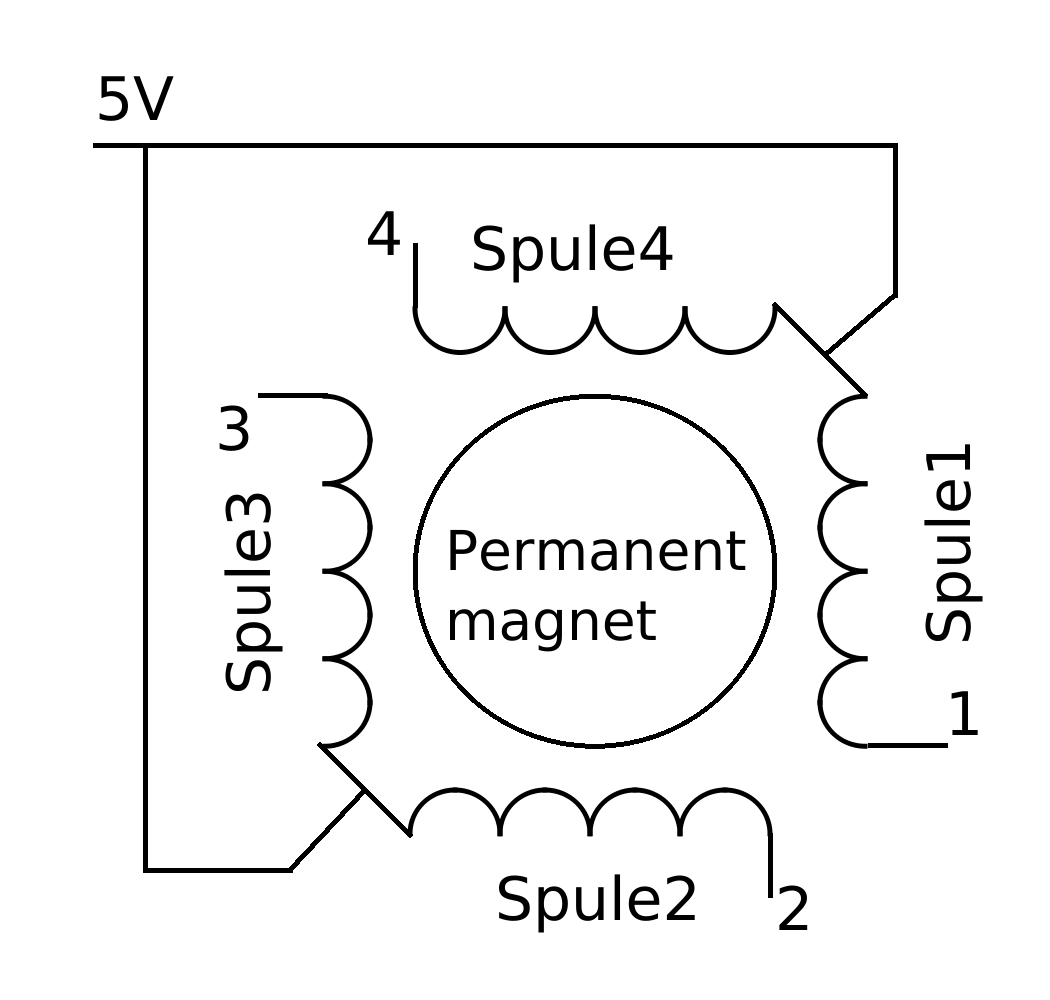
\includegraphics[width=\textwidth]{./Zeichnungen/schaltplan-schrittmotor-innen.png}
		\caption{Schaltplan zu den Spulen.}
	\end{figure}
\end{minipage}

\bigskip
In der Mitte der Spulen befindet sich ein Permanentmagnet, an dessen Ende ein Zahnrad angebracht ist, das wiederum weitere Zahnräder in Bewegung versetzt. Die Spulen werden nun abwechselnd an und aus geschaltet und wirken dabei als Elektromagnet. Durch die wechselnde Anziehung und Abstoßung des Permanentmagneten in der Mitte beginnt dieser, sich zu drehen.
\marginpar{\video \\ \scriptsize \href{https://www.youtube.com/watch?v=Vtbd80FksuM}{Funktions-weise eines Schrittmotors}}
Für das Ein- und Ausschalten der Spulen wird ein Motortreiber genutzt, der den Arduino vor zu hohen und rückläufigen Strömen schützt (vgl. Abschnitt \ref{sec:motoren}). Aufgrund der Stromaufnahme von ca. $\SI{240}{\milli\ampere}$ ist es empfehlenswert, eine externe Spannungsversorgung am Motortreiber anzuschließen (zum Beispiel mit Hilfe des \emph{Power Supply Module}, vgl. S.\, \pageref{powersupplymodule} - denke an die gemeinsame Erdung mit dem Arduino!). Da die Spulen auch beim Halten der Position dauerhaft unter Strom stehen müssen, ist der Stromverbrauch konstant hoch.

% Bild: Schaltplan mit Motortreiber
\begin{figure}[h]
	\centering
	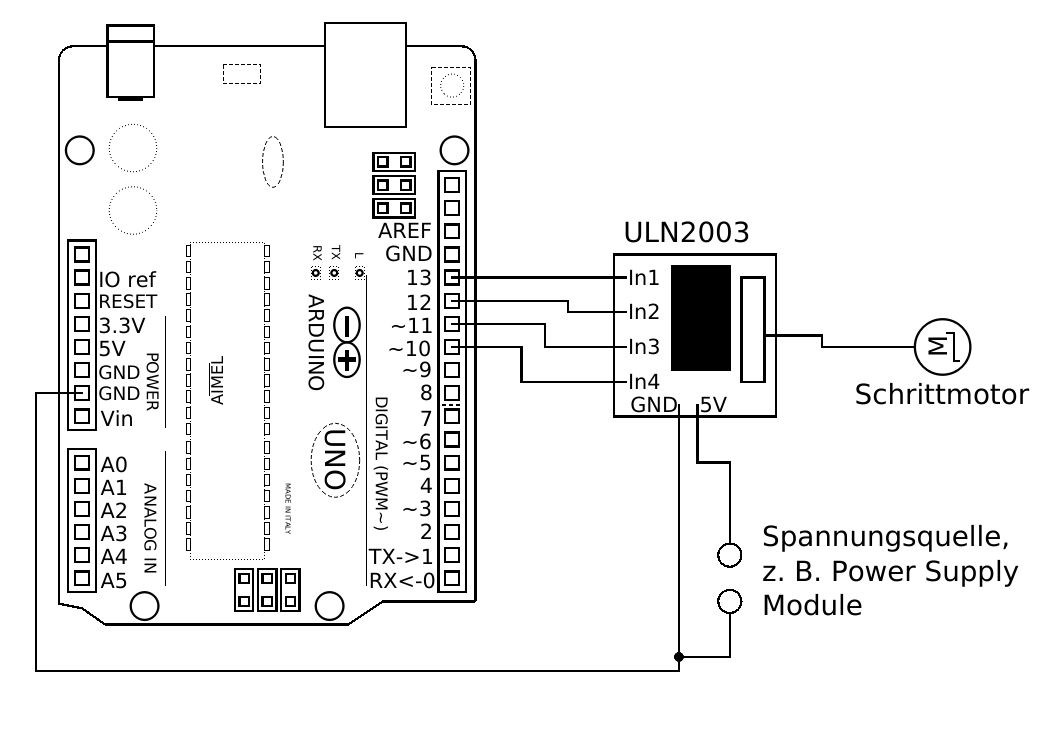
\includegraphics[width=0.8\textwidth]{./Zeichnungen/schaltplan-schrittmotor-anschluss.png}
	\caption{Anschluss des Schrittmotors an den Motortreiber ULN2003 und den Arduino mit externer Spannungsquelle.}
\end{figure}
Die korrekte Reihenfolge des Ein- und Ausschaltens der Spulen ist bereits in Nepo implementiert, sodass die Steuerung sich einfach bewerkstelligen lässt. Es ist aber wichtig zu verstehen, dass jede Spuleneinstellung den Permanentmagneten in der Mitte dazu bringt, sich um einen kleinen Winkel zu drehen. Dieser Winkel wird auch Schritt genannt und dies gibt dem Schrittmotor seinen Namen. Dieser Schritt oder Winkel ist auch die kleinste Schrittweite, die der Motor ansteuern kann und gibt somit die Präzision des Motors an. Beim hier verwendeten Modell 28BYJ-48 beträgt der Schrittwinkel $\ang{5,625}$ (vgl. \href{https://components101.com/motors/28byj-48-stepper-motor}{Datenblatt}), woraus sich ergibt, dass der Motor 64 Schritte für eine Umdrehung benötigt. Durch die eingebauten Zahnräder wird die Drehung des Schafts aber weiter verlangsamt, sodass ein Motorschritt nur einer Schaftdrehung von etwa $\ang{0,176}$ (1/32 der Motorschrittweite) entspricht. Dies bedeutet, dass der Motor 2048 Schritte für eine Umdrehung braucht. Wenn du in den textbasierten Quellcode von Nepo schaust, nachdem du einen Schrittmotor konfiguriert hast, wirst du diese Zahl wiederfinden!
% Bild von Befehlen
\begin{figure}[h]
	\centering
	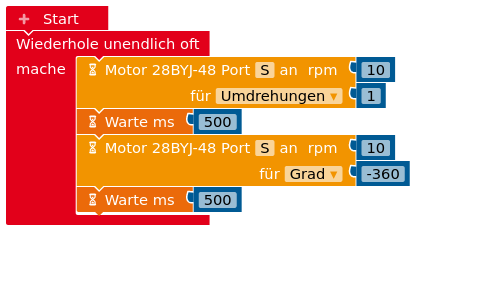
\includegraphics[width=0.65\textwidth]{./pics/schrittmotor-steuerung.png}
	\vspace{-\baselineskip}
\end{figure}
In Nepo lässt sich einfach angeben, mit welcher Geschwindigkeit (in Umdrehungen pro Minute, engl. \emph{revolutions per minute, rpm}) und um wie viele Umdrehungen sich der Schaft drehen soll. Alternativ kann angegeben werden, um wie viel Grad sich der Schaft drehen soll.

\begin{projekt}[Sekundenzeiger]\label{proj:sekundenzeiger}
	Programmiere einen möglichst präzisen Sekundenzeiger. Überprüfe ihn mit der Stoppuhr deines Smartphones.
	
	Tipp: Nutze Klebeband, um eine kleine Fahne als Zeiger zu basteln.
\end{projekt}


%\begin{projekt}[Fensterheber]\label{proj:fensterheber}
%	Der Fensterheber eines Autos hat üblicherweise zwei Funktionen:	
%	\begin{enumerate}[label=(\alph*), itemsep=0mm, parsep=0mm]
%		\item Wenn man den Schalter halb hochzieht bzw. herunterdrückt, wird das Fenster so lange angehoben bzw. abgesenkt, wie der Schalter in dieser Position verbleibt.
%		\item Wenn der Schalter ganz hochgezogen bzw. heruntergedrückt wird, wird das Fenster auch ganz hochgehoben bzw. heruntergefahren.
%	\end{enumerate}
%	
%	Modelliere eine Funktion des Fensterhebers mit zwei Tastern (mit Widerstand! - vgl. Abschnitt \ref{sec:taster}) und einem Schrittmotor. Wenn du beide Funktionen modellieren willst, brauchst du vier Taster (mit Widerstand!).
%\end{projekt}


\newpage
\section{Liquid Crystal Display (LCD)}
\label{sec:lcd}
\setcounter{aufgabennummer}{0}
\setcounter{projektnummer}{0}
%kurze Übersicht der Befehle
% Hintergrundinfo: Physikalisch - wie werden Pixel sichtbar; informatisch - wie werden Zeichen durch Bitfolgen definiert
% eigene Zeichen definieren: Bsp und Aufgabe
%kein eigenes Projekt: lässt sich bei quasi allen anderen Projekten einbinden

\begin{wrapfigure}{r}{0.3\textwidth}
	\centering
	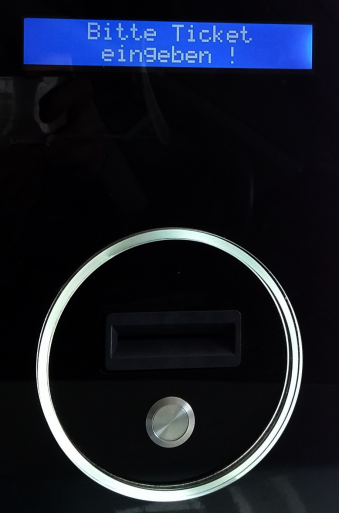
\includegraphics[width=0.3\textwidth]{./pics/lcd-im-parkhaus-v2.png}
	\caption{LC-Display an einem Parkhaus-Automaten.}
	\label{abb:lcd-parkhaus}
	\vspace{-2\baselineskip}
\end{wrapfigure}
In vielen Projekten genügt es nicht, Messwerte, Statusanzeigen oder Menüs über den seriellen Monitor am Computer anzeigen zu lassen - man benötigt stattdessen ein Display, das sich direkt an den Arduino anschließen und mit ihm verbauen lässt. Ein günstige Möglichkeit dafür bieten sogenannte \textbf{L}iquid \textbf{C}rystal \textbf{D}isplays (LCD), die man zum Beispiel in Kaffeemaschinen oder Parkautomaten finden kann (siehe B\ref{abb:lcd-parkhaus}). Modernere LCD werden in Laptops, Fernsehern und Tablets verbaut.

Um ein LC-Display anzusteuern, werden ziemlich viele Kabel benötigt. Daher gibt es neben den normalen LC-Displays häufig auch eine Variante, bei der ein I2C-Modul am LC-Display angebracht ist, was die benötigten Kabel deutlich reduziert. Im Folgenden werden beide Varianten beschrieben.

\vspace{3\baselineskip}
\emph{LC-Display ohne I2C-Modul}

Im Schaltplan sind die Kabel so mit dem Arduino verbunden, wie es die Standardkonfiguration für das LCD 1602 in Nepo angibt. Es empfiehlt sich, die zahlreichen 5V- und GND-Anschlüsse auf den Längsseiten des Steckbretts zu sammeln.

\bigskip
\begin{minipage}{0.64\textwidth}
	\centering
	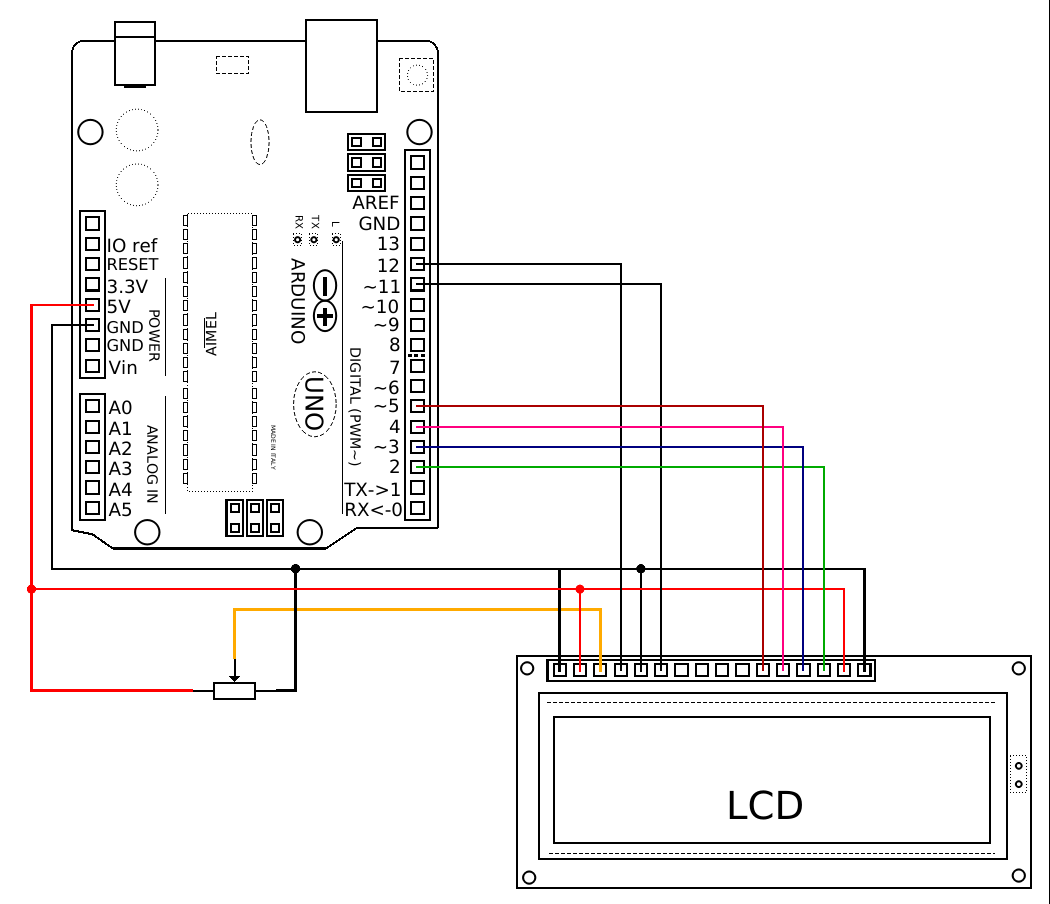
\includegraphics[width=\textwidth]{./Zeichnungen/schaltplan-lcd-ohne-i2c.png}
\end{minipage}
\hfill
\begin{minipage}{0.34\textwidth}
	\small
	\centering
	\begin{tabular}{c|c}
		\textbf{LCD} & \textbf{Arduino} \\ \hline
		VSS & GND \\ \hline
		VDD & 5V \\ \hline
		V0 & Drehregler (Mitte)\\ \hline
		RS & 12\\ \hline
		RW & GND\\ \hline
		E & 11\\ \hline
		D0 - D3 & -- \\ \hline
		D4 & 5\\ \hline
		D5 & 4\\ \hline
		D6 & 3\\ \hline
		D7 & 2\\ \hline
		A & 5V\\ \hline
		K & GND\\ \hline
	\end{tabular}
\end{minipage}

\bigskip
Die Anschlüsse A und K stehen für die Anode und Kathode der LEDs, die die Hintergrundbeleuchtung ausmachen. Mit dem Drehregler wird der Kontrast des Bildschirms eingestellt.

\newpage
\emph{LCD mit I2C-Modul}

Die I2C-Schnittstelle erlaubt es, ein LC-Display mit nur vier Kabel anzusteuern. Der Anschluss an den Arduino erfolgt wie in der Abbildung dargestellt.

\begin{figure}[H]
	\centering
	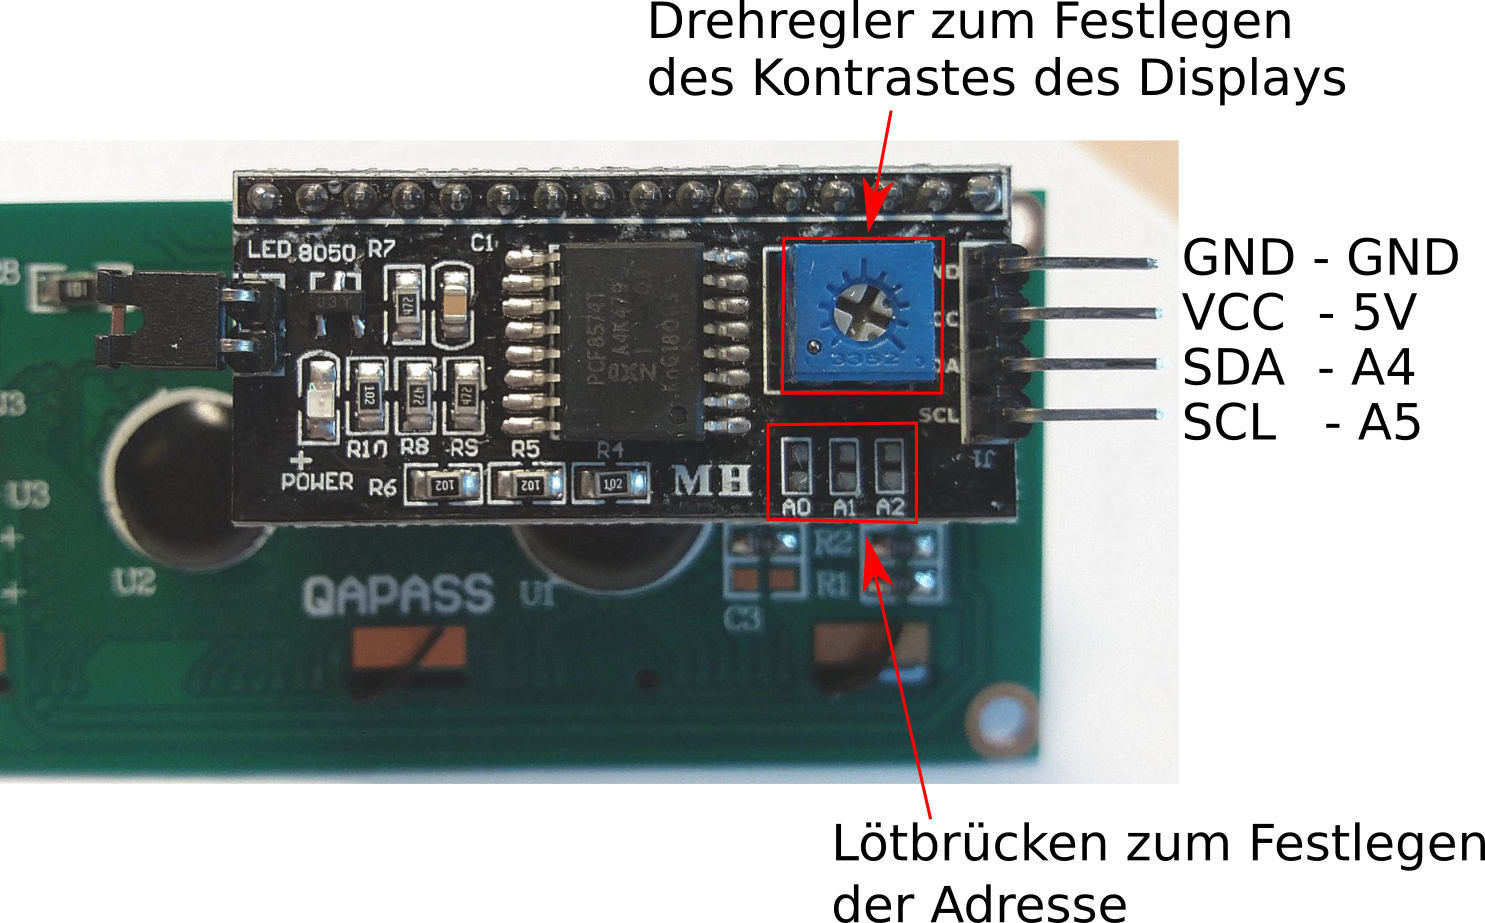
\includegraphics[width=0.55\textwidth]{./pics/i2c-modul-beschriftet.png}
\end{figure}

\begin{zsfg}{I2C oder IIC: Inter-Integrated Circuit}
	I2C steht für \emph{\href{https://de.wikipedia.org/wiki/I\%C2\%B2C}{Inter-Intergrated-Circuit}}. Dies ist ein sogenannter Datenbus, also ein System zur Übertragung von Daten zwischen mehreren Teilnehmern. Die Datenübertragung funktioniert über ein getaktetes An- und Ausstellen der Datenleitung, um die Daten in Binärform (1 und 0) zu übertragen. Neben der Spannungsversorgung (GND und VCC) wird dazu ein Kabel für die serielle Datenübertragung (SDA - Serial Data) und ein Kabel für die Abstimmung des Taktes (SCL - Serial Clock) benötigt.
	
	\begin{wrapfigure}{r}{0.5\textwidth}
		\centering
		\vspace{-0.5\baselineskip}
		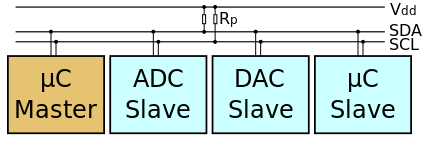
\includegraphics[width=0.45\textwidth]{./pics/i2c-info.png}
		\caption{I2C-Bus mit einem Master- und drei Slave-Geräten (Quelle: \href{https://de.wikipedia.org/wiki/Datei:I2C.svg}{Wikipedia}, \href{https://creativecommons.org/licenses/by-sa/3.0/deed.de}{CC BY-SA 3.0}, Urheber: \href{https://en.wikipedia.org/wiki/User:Cburnett}{Colin Burnett}).}
		\vspace{-0.5\baselineskip}
	\end{wrapfigure}
	Da auch mehrere I2C-kompatible Geräte an denselben Datenbus angeschlossen werden können, bekommt jedes Gerät eine Adresse, damit klar ist, welches Gerät die Daten bekommen soll. Die Adresse wird bei der Konfiguration als Hexadezimalzahl angegeben und kann prinzipiell zwischen 0 und 127 liegen. Typischerweise ist die voreingestellte Adresse \texttt{0x27}. Dabei bedeutet \texttt{0x}, dass die folgenden beiden Ziffern als Hexadezimalzahl zu interpretieren sind. Falls bereits ein anderes Gerät auf dem gleichen Datenbus dieselbe Adresse hat, kann die Adresse über die Lötbrücken verändert werden (siehe \href{https://www.bastelgarage.ch/i2c-schnittstelle-pcf8574-fur-lcd-display}{bastelgarage.ch}).
\end{zsfg}

\bigskip
\begin{aufgabe}\emph{Funktionstest}
	
	Schließe das LC-Display wie beschrieben an den Arduino an und erstelle ein Programm, das \enquote{Hello World!} auf dem LC-Display anzeigt.
	
	\emph{Hinweis:} Falls alle Pixel weiß oder blau bleiben, kann es sein, dass der Drehregler falsch eingestellt ist. Drehe in diesem Fall an dem Drehregler, um den Kontrast zu verbessern. Für den Drehregler auf dem I2C-Modul (blauer Kasten) brauchst du einen Schraubenzieher o. ä.
\end{aufgabe}
%\begin{minipage}{0.64\textwidth}
%	\begin{aufgabe}\emph{Funktionstest}
%		
%		Schließe das LC-Display wie beschrieben an den Arduino an und erstelle mithilfe der LCD-Extension ein Programm, das \enquote{Hello World!} auf dem LC-Display anzeigt.
%		
%		\emph{Hinweis:} Falls alle Pixel weiß bleiben oder auf dem LCD gar nichts zu sehen ist, kann es sein, dass der Drehregler falsch eingestellt ist. Drehe in diesem Fall an dem Drehregler, um den Kontrast zu verbessern.
%	\end{aufgabe}
%\end{minipage}
%\hfill
%\begin{minipage}{0.34\textwidth}
%	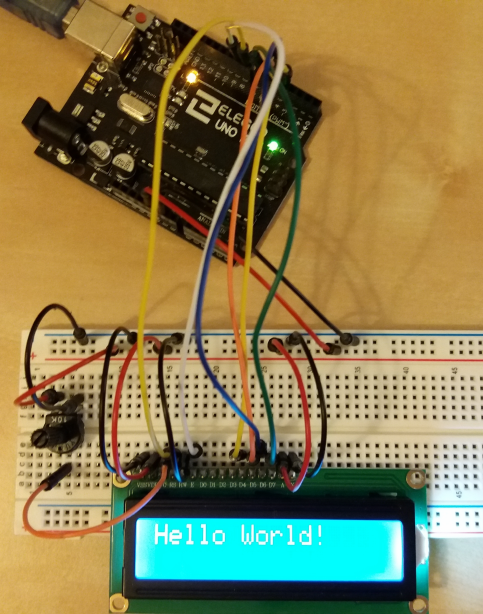
\includegraphics[width=\textwidth]{./pics/arduino-lcd-klein.png}
%\end{minipage}

% Aufgabe: ständig aktualisierte Anzeige eines Zahlenwertes von 1 bis 300 (rechtsbündig) mit Einheit
\begin{aufgabe} \emph{Messwertanzeige}
	
	In vielen Anwendungen soll auf dem LC-Display ein Messwert o.\,ä. angezeigt werden, der sich mit der Zeit ändern kann. Diese Anzeige soll aber schön formatiert sein.
	
	Erstelle ein Programm, das alle drei Sekunden eine Zufallszahl \texttt{z} zwischen 0 und 200 erzeugt und auf dem Display folgende Anzeige ausgibt:
	
	\begin{center}
		\texttt{Messwert: z E}
	\end{center}
	
	\emph{Hinweise:}
	\begin{itemize}[itemsep=0mm, parsep=0mm]
		\item \texttt{E} soll für eine beliebige Einheit stehen.
		\item Achte darauf, dass der vorherige Wert von \texttt{z} gelöscht wird (\button{lcd clear}).
		\item Die Ausgabe der Zahl \texttt{z} soll immer rechtsbündig erfolgen, sodass zwischen den Einern von \texttt{z} und der Einheit genau ein Leerzeichen steht.
		\item Du benötigst den Befehl \button{LCD set cursor (line <\_> position <\_>)}. Darin steht \texttt{line} für die Zeile, deren Nummer entweder $0$ (oben) oder $1$ (unten) ist. \texttt{position} steht für die Spalte, deren Nummer sich von $0$ bis $15$ erstrecken kann. (In der Informatik beginnt das Zählen stets mit der Null!)		
	\end{itemize}
\end{aufgabe}

\begin{aufgabe} \emph{Codierung von Zeichen auf dem LCD}
	
	Für die Darstellung von Zeichen auf dem LCD muss im Hintergrund geklärt werden, welche Pixel an- und ausgestellt werden müssen. Dazu lohnt ein genauer Blick auf die Zellen des LCD.
	
	Jede Zelle besteht aus $5 \times 8$ Pixeln, von denen manche weiß und manche blau sind. Wenn man für jedes Pixel eine \texttt{1} (weiß) oder eine \texttt{0} (blau) notiert, dann erhält man Bitfolgen (gekennzeichnet durch das vorstehende \texttt{0b}), die sich in einer Reihung notieren lassen.
	
	\begin{figure}[H]
		\centering
		\footnotesize
		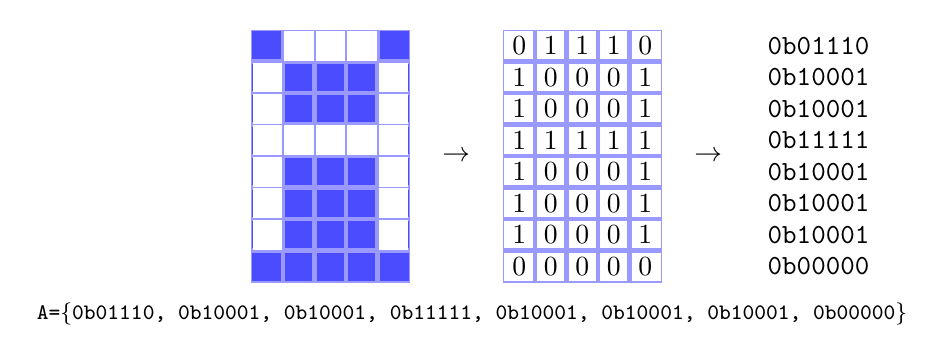
\begin{tikzpicture}[scale=0.4]
		%%%% Zelle auf LCD
		\filldraw[fill=blue!70,draw=blue!40] (0,0) rectangle (5,8);
		\foreach \x in {1,...,4} {
			\draw [blue!40,ultra thick] (\x , 0) -- (\x,8);
		}
		\foreach \y in {1,...,7} {
			\draw [blue!40,ultra thick] (0,\y) -- (5,\y);
		}
		% Zeichen A
		\foreach \x in {0.5,4.5} {
			\foreach \y in {1.5,...,6.5} {
				\fill[white] (\x-0.47,\y-0.47) rectangle (\x+0.47,\y+0.47);
			}
		}
		\foreach \x in {1.5,2.5,3.5} {
			\foreach \y in {4.5,7.5} {
				\fill[white] (\x-0.47,\y-0.47) rectangle (\x+0.47,\y+0.47);
			}
		}
		% Pfeil
		\node at (6.5,4) {$\rightarrow$};
		%%%% Zelle auf LCD codiert
		\filldraw[fill=white,draw=blue!40] (8,0) rectangle (13,8);
		\foreach \x in {9,...,12} {
			\draw [blue!40,ultra thick] (\x , 0) -- (\x,8);
		}
		\foreach \y in {1,...,7} {
			\draw [blue!40,ultra thick] (8,\y) -- (13,\y);
		}
		%Zeichen A codiert
		\foreach \x in {8.5,12.5} {
			\foreach \y in {1.5,...,6.5} {
				\node at (\x,\y) {1};
			}
		}
		\foreach \x in {9.5,10.5,11.5} {
			\foreach \y in {4.5,7.5} {
				\node at (\x,\y) {1};
			}
		}
		\foreach \x in {9.5,10.5,11.5} {
			\foreach \y in {0.5,...,3.5,5.5,6.5} {
				\node at (\x,\y) {0};
			}
		}
		\foreach \x in {8.5,12.5} {
			\foreach \y in {0.5,7.5} {
				\node at (\x,\y) {0};
			}
		}
		% Pfeil
		\node at (14.5,4) {$\rightarrow$};
		%%%% Bitfolgen
		\node at (18,7.5) {\texttt{0b01110}};
		\node at (18,6.5) {\texttt{0b10001}};
		\node at (18,5.5) {\texttt{0b10001}};
		\node at (18,4.5) {\texttt{0b11111}};
		\node at (18,3.5) {\texttt{0b10001}};
		\node at (18,2.5) {\texttt{0b10001}};
		\node at (18,1.5) {\texttt{0b10001}};
		\node at (18,0.5) {\texttt{0b00000}};
		%Zusammenfassung
		\node at (7,-1) {\footnotesize \texttt{A=\{0b01110, 0b10001, 0b10001, 0b11111, 0b10001, 0b10001, 0b10001, 0b00000\}}};
		\end{tikzpicture}
		\caption{Codierung des Buchstabens A auf einem LC-Display.}
	\end{figure}
	
	Man könnte die Reihung von Bitfolgen auch als Reihung von Dezimalzahlen notieren und käme auf das gleiche Ergebnis. Das macht den Code zwar kürzer, jedoch leidet die Lesbarkeit des Codes deutlich.
	
	\emph{Entwerfe einen Smiley und ein eigenes Symbol auf $5 \times 8$ Pixeln und notiere die zugehörige Reihung von Bitfolgen, die dieses Zeichen codiert.}
	
	\emph{Hinweis:} Mit der textbasierten Arduino-IDE lassen sich nach dem oben beschriebenen Prinzip auch eigene Zeichen für das LC-Display codieren. Ein Beispiel findet sich unter \texttt{Datei} $\rightarrow$ \texttt{Beispiele} $\rightarrow$ \texttt{LiquidCrystal} $\rightarrow$ \texttt{CustomCharacter}.
\end{aufgabe}


\newpage
\section{Neigungsschalter}
\label{sec:neigungsschalter}
\setcounter{aufgabennummer}{0}
\setcounter{projektnummer}{0}

\begin{wrapfigure}{r}{0.2\textwidth}
	\centering
	\vspace{-\baselineskip}
	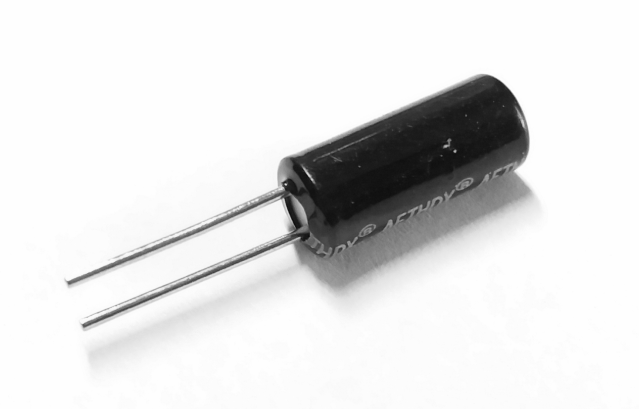
\includegraphics[width=0.2\textwidth]{./pics/neigungsschalter.png}
	\caption{Neigungsschalter.}
	\vspace{-\baselineskip}
\end{wrapfigure}
Mit sogenannten Neigungsschaltern (engl. \emph{tilt switch}) lässt sich eine Neigung, aber auch eine Erschütterung oder der Beginn einer Beschleunigung messen. So lässt sich zum Beispiel feststellen, ob ein Gegenstand angehoben wird.

\begin{ziel}
	\textbf{Ziel:} Es soll eine Alarmanlage gebaut werden, die auslöst, wenn das Steckbrett angehoben wird.
\end{ziel}

\medskip
\begin{aufgabe}
	
	\medskip
	\begin{minipage}{0.59\textwidth}
		Die Abbildung rechts zeigt den Aufbau eines Neigungsschalters im geschlossenen und geöffneten Fall. Beschreibe den Aufbau des Schalters und erkläre, wie es in Abhängigkeit der Neigung des Neigungsschalters zum Leuchten der LED in Abbildung \ref{abb:neigungsschalter-einfach} kommt. Handelt es sich um einen digitalen oder analogen Sensor?
		
		\begin{figure}[H]
			\centering
			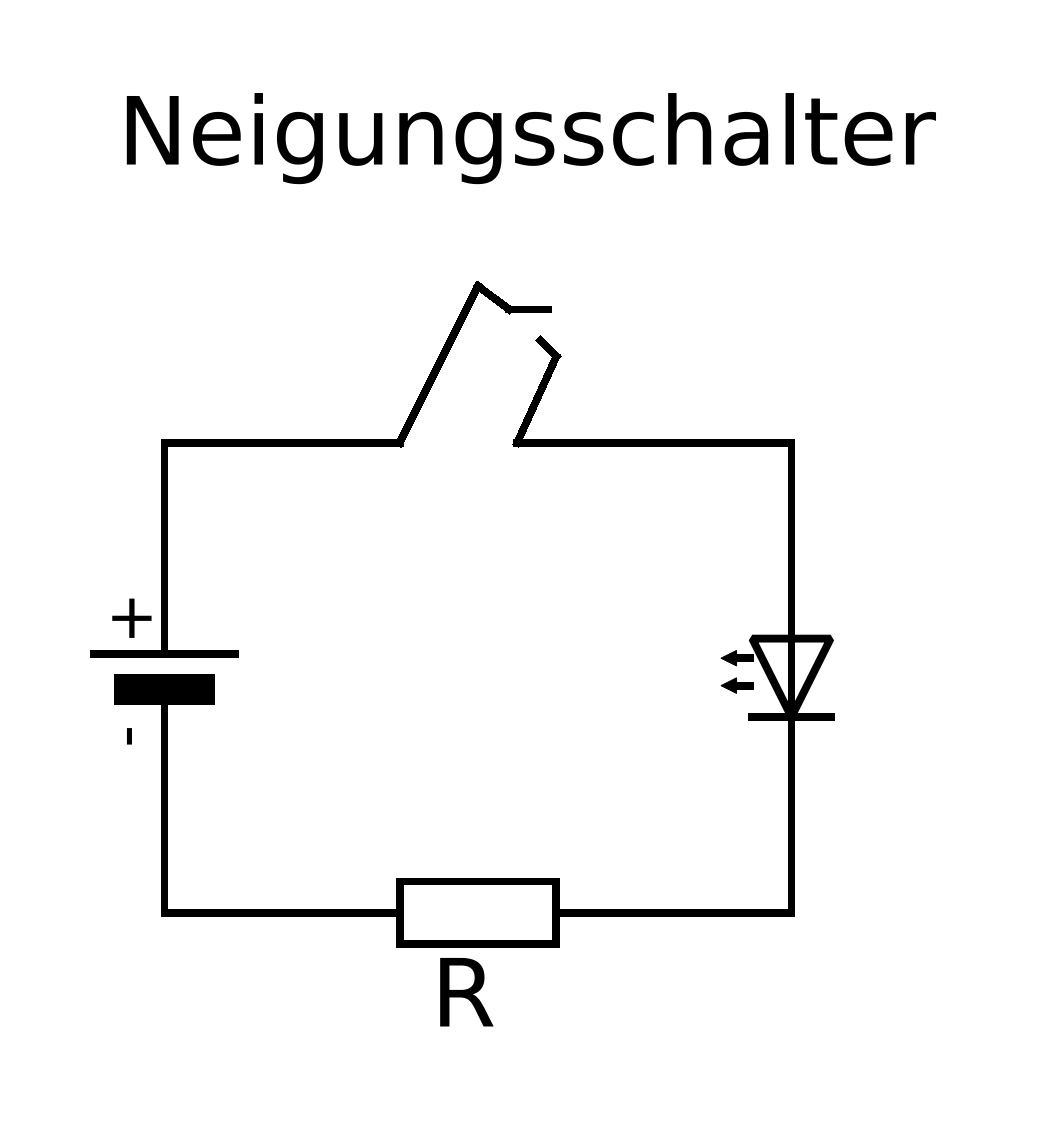
\includegraphics[width=0.4\textwidth]{./Zeichnungen/neigungsschalter-einfach.png}
			\caption{Einfacher Aufbau zum Test eines Neigungsschalters ohne Arduino.}
			\label{abb:neigungsschalter-einfach}
		\end{figure}
	\end{minipage}
	\hfill
	\begin{minipage}{0.39\textwidth}
		\begin{figure}[H]
			\centering
			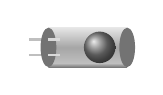
\begin{tikzpicture}
			% Kontaktstifte außen
			\draw [thick, gray!50] (-0.25,0.15) -- (0,0.15);
			\draw [thick, gray!50] (-0.25,0.35) -- (0,0.35);
			% Wände
			\shade [bottom color=gray!95!black, top color=gray!50] (0,0) rectangle (1,0.05);
			\shade [bottom color=gray!50, top color=gray!70] (0,0.05) rectangle (1,0.25);
			\shade [bottom color=gray!70, top color=gray!20] (0,0.25) rectangle (1,0.5);
			% Boden und Deckel
			\fill[gray!90!black] (0,0.25) ellipse [y radius=0.25, x radius=0.1];
			\fill[gray!90!black] (1,0.25) ellipse [y radius=0.25, x radius=0.1];
			% Kontaktstifte innen
			\draw [thick, gray!30] (0,0.15) -- (0.15,0.15);
			\draw [thick, gray!30] (0,0.35) -- (0.15,0.35);
			% Kugel
			\shade [ball color=gray] (0.65,0.25) circle [radius=0.2];
			\end{tikzpicture}
			\caption{Neigungsschalter (geöffnet).}
		\end{figure}
		
		\begin{figure}[H]
			\centering
			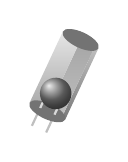
\begin{tikzpicture}[rotate=65]
			% Kontaktstifte außen
			\draw [thick, gray!50] (-0.25,0.15) -- (0,0.15);
			\draw [thick, gray!50] (-0.25,0.35) -- (0,0.35);
			% Wände
			\shade [bottom color=gray!95!black, top color=gray!50] (0,0) rectangle (1,0.05);
			\shade [bottom color=gray!50, top color=gray!70] (0,0.05) rectangle (1,0.25);
			\shade [bottom color=gray!70, top color=gray!20] (0,0.25) rectangle (1,0.5);
			% Boden und Deckel
			\fill[gray!90!black] (0,0.25) ellipse [y radius=0.25, x radius=0.1];
			\fill[gray!90!black] (1,0.25) ellipse [y radius=0.25, x radius=0.1];
			% Kontaktstifte innen
			\draw [thick, gray!30] (0,0.15) -- (0.15,0.15);
			\draw [thick, gray!30] (0,0.35) -- (0.15,0.35);
			% Kugel
			\shade [ball color=gray] (0.25,0.25) circle [radius=0.2];
			\end{tikzpicture}
			\caption{Neigungsschalter (geschlossen).}
		\end{figure}
	\end{minipage}
\end{aufgabe}

\vspace{2\baselineskip}

\begin{wrapfigure}{r}{0.6\textwidth}
	\centering
	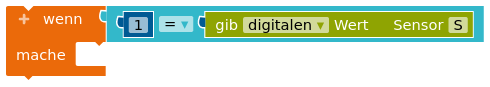
\includegraphics[width=0.55\textwidth]{./pics/digitalen-sensor-auslesen.png}
\end{wrapfigure}
\emph{Programmierung:} Der Neigungsschalter ist in Nepo nicht vorkonfiguriert, aber dies ist auch gar nicht nötig. Er lässt sich als digitaler Sensor konfigurieren. Der Rückgabewert eines digitalen Sensors ist in Nepo vom Typ \emph{Zahl} statt vom Typ \emph{Wahrheitswert}. Dabei bedeutet die Zahl \texttt{0} so viel wie \texttt{false} und die Zahl \texttt{1} bedeutet \texttt{true}.
\vfill

\newpage
\begin{minipage}[t]{0.55\textwidth}
	\begin{projekt}[Alarmanlage]\label{proj:neigungsalarmanlage}
		Baue eine Alarmanlage, die auslöst, wenn das Steckbrett angehoben wird.
		
		\emph{Hinweis:} Wenn der Neigungsschalter wie rechts abgebildet am Arduino angeschlossen wird, kann sein Zustand in Digitalpin 3 ausgelesen werden (vgl. das \hyperref[abb:schaltplan-taster-pulldown]{Auslesen von Tastern}).
		
		\emph{Zusatz:} Erkläre, warum es sinnvoll ist, den Piezo-Summer nicht so wie die LED in Abb.\,\ref{abb:neigungsschalter-einfach} direkt mit dem Neigungsschalter zu verbinden, sondern das Auslösen des Tons im Programm zu regeln.
	\end{projekt}
\end{minipage}
\hfill
\begin{minipage}[t]{0.44\textwidth}
	\begin{figure}[H]
		\centering
		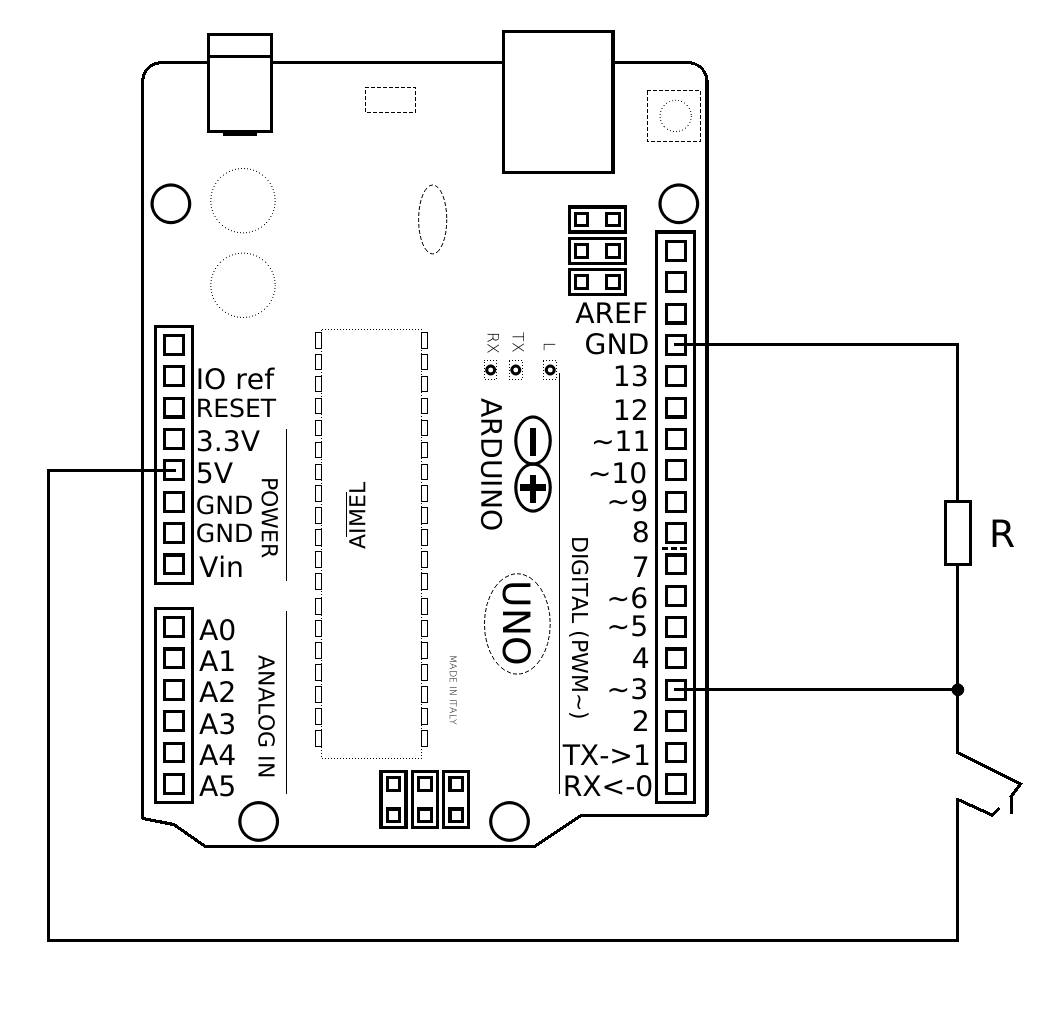
\includegraphics[width=\textwidth]{./Zeichnungen/neigungsschalter-mit-arduino.png}
	\end{figure}
\end{minipage}


\newpage
\section{Bewegungsmelder}
\label{sec:bewegungsmelder}

\emph{Bewegungsmelder wurden bereits in Abschnitt \ref{sec:wahrheitswerte} erklärt und genutzt, um Wahrheitswerte einzuführen. In diesem Abschnitt steht das Bauteil im Vordergrund. Dazu werden noch einmal alle Informationen zusammengefasst und eine alternative Programmierung vorgestellt.}
\bigskip

\begin{wrapfigure}{r}{0.3\textwidth}
	\centering
	\vspace{-\baselineskip}
	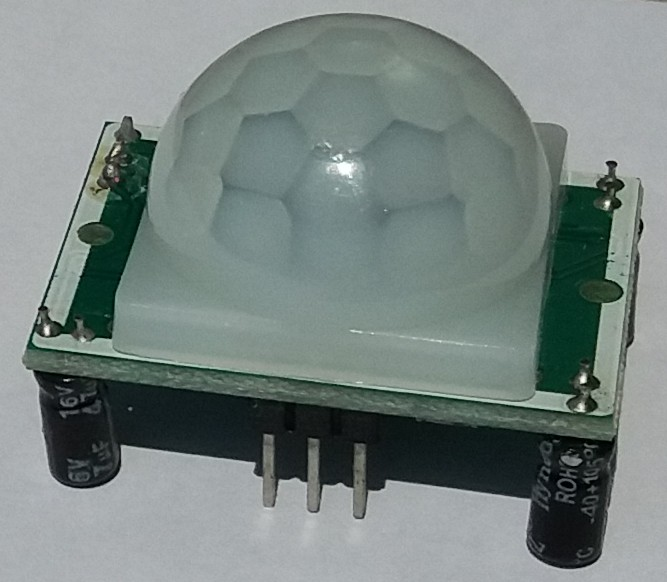
\includegraphics[width=0.2\textwidth]{./pics/bewegungsmelder.jpg}
	\label{abb:bewegungsmelder2}
	\vspace{-\baselineskip}
\end{wrapfigure}
Bewegungsmelder verfügen über drei Pins, deren Beschriftung man lesen kann, wenn man die Kunststofflinse vorsichtig abzieht (\emph{Vorsicht: Nach Abziehen der Linse nicht den Sensor berühren!}). \texttt{Vcc} und \texttt{GND} dienen der Stromversorgung der elektronischen Komponenten und müssen mit \texttt{5\,V} und \texttt{GND} am Arduino verbunden werden. 

\begin{wrapfigure}{r}{0.3\textwidth}
	\centering
	\vspace{-0.5\baselineskip}
	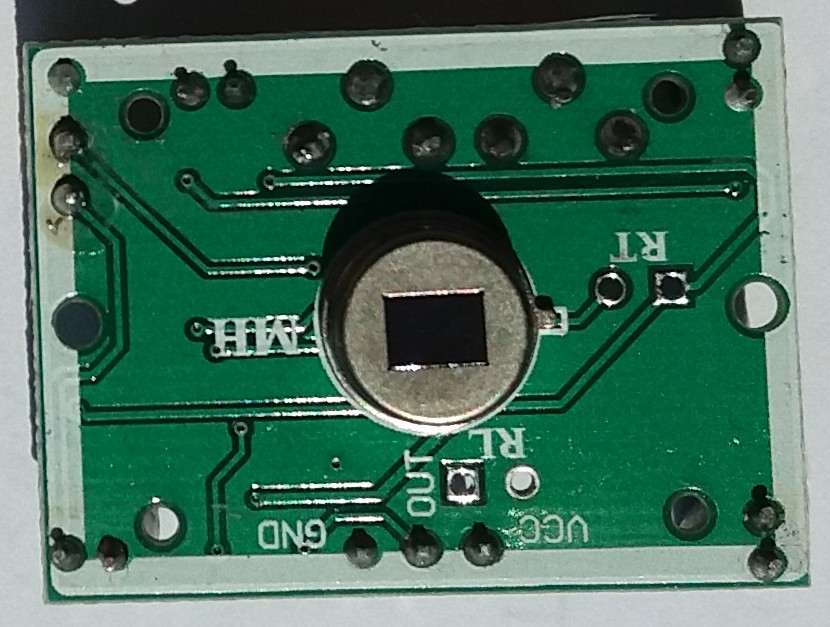
\includegraphics[width=0.25\textwidth]{pics/bewegungsmelder-ohne-linse.jpg}
	\label{abb:bewegungsmelder-ohne-linse2}
	\vspace{-0.5\baselineskip}
\end{wrapfigure}
Der mittlere \texttt{OUT}-Pin ist der Signal-Pin: Wenn eine Bewegung registriert wurde, liegt er auf einem hohen elektrischen Potential (\texttt{HIGH}); wenn keine Bewegung registriert wurde, liegt er auf einem niedrigen elektrischen Potential (\texttt{LOW}). Zum Einlesen des Signals wird dieser Pin mit einem digitalen Pin des Arduino verbunden, der dann digitaler Eingang heißt.

\begin{wrapfigure}{r}{0.3\textwidth}
	\centering
	\vspace{-0.75\baselineskip}
	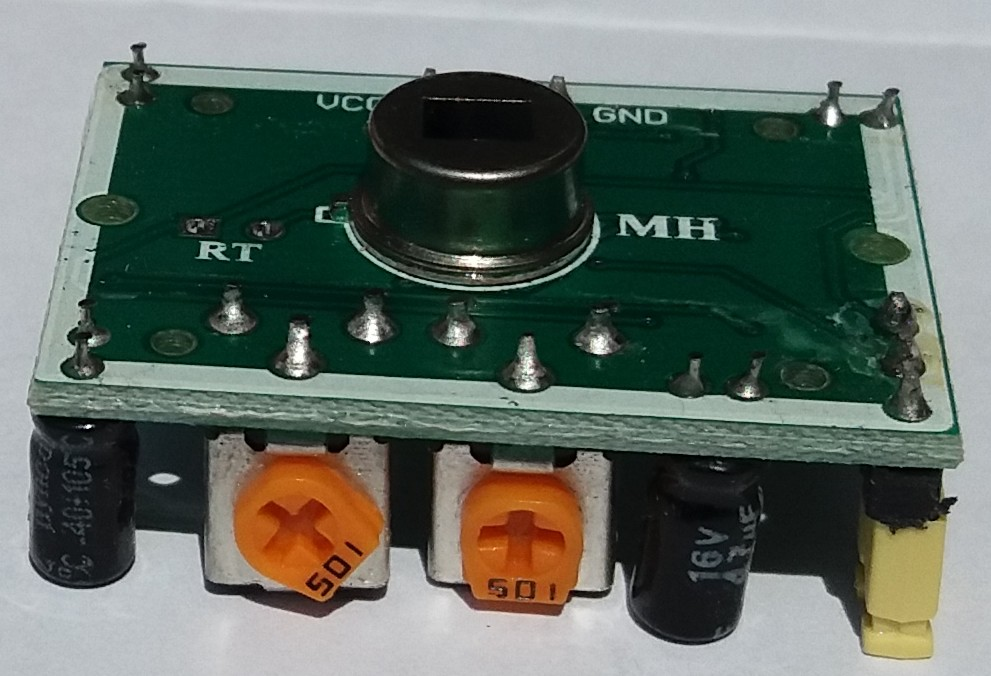
\includegraphics[width=0.25\textwidth]{pics/bewegungsmelder-hinten.jpg}
	\vspace{-\baselineskip}
	\label{abb:bewegungsmelder-hinten2}
\end{wrapfigure}
Hinten befinden sich zwei Drehregler (\enquote{Potentiometer}), mit denen sich die Dauer des Bewegungssignals (links) und die Empfindlichkeit (rechts) einstellen lassen. Zusätzlich befindet sich auf der rechten Seite ein sogenannter Jumper, mit dem auf einfache Weise eine Steckverbindung zwischen benachbarten Pins hergestellt werden kann. Wenn sich der Jumper ganz außen befindet, dann bleibt das Bewegungssignal nach dem Erkennen einer Bewegung eine Weile aktiv und wird dann auf jeden Fall deaktiviert. Eine neue Bewegung kann erst nach einer gewissen Zeit wieder registriert werden. Wenn der Jumper hingegen leicht nach innen versetzt ist, bleibt das Bewegungssignal so lange erhalten, wie eine Bewegung erkannt wird (siehe \href{https://funduino.de/nr-8-bewegungsmelder}{Funduino.de}).

\bigskip

\begin{wrapfigure}{r}{0.6\textwidth}
	\centering
	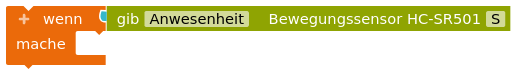
\includegraphics[width=0.55\textwidth]{./pics/bewegungsmelder-auslesen.png}
	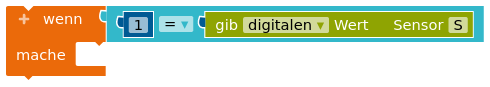
\includegraphics[width=0.55\textwidth]{./pics/digitalen-sensor-auslesen.png}
	\caption{Zwei Varianten zum Auslesen eines Bewegungsmelders. Oben wurde die Konfiguration als Bewegungsmelder vorgenommen, unten als digitaler Sensor.}
\end{wrapfigure}
\emph{Programmierung:} Der Bewegungsmelder ist in Nepo bereits vorkonfiguriert und lässt sich damit einfach auslesen. Aufgrund der Ausgabe von \texttt{HIGH} und \texttt{LOW} bzw. \texttt{true} und \texttt{false} lässt er sich aber auch als digitaler Sensor konfigurieren. Der Rückgabewert eines digitalen Sensors ist in Nepo vom Typ \emph{Zahl} statt vom Typ \emph{Wahrheitswert}. Dabei bedeutet die Zahl \texttt{0} so viel wie \texttt{false} und die Zahl \texttt{1} bedeutet \texttt{true}.

\begin{projekt}[Automatische Tür]\label{proj:tueroeffner}
	Baue und programmiere eine automatische Tür, die sich öffnet, wenn eine Bewegung registriert wird. Der Bewegungsmelder soll als digitaler Sensor konfiguriert werden. Experimentiere mit den Drehreglern, um die Empfindlichkeit und Dauer des Signals richtig einzustellen.
\end{projekt}

\begin{recherche}{Wie funktioniert eigentlich ein Bewegungsmelder?}
	Das zentrale Bauteil eines Bewegungsmelders ist ein sogenannter \emph{Passiver Infrarot Sensor (PIR)}, auch \emph{Pyroelektrischer Sensor}. Recherchiere im Internet, wie solche Sensoren funktionieren und fasse zusammen, wie es zur Registrierung einer Bewegung kommt.	
\end{recherche}


\newpage
\section{Joystick}
\label{sec:joystick}

Joysticks werden bekanntermaßen für Spielecontroller oder auch zur Steuerung von Maschinen genutzt. Mit dem Arduino lassen sich einfache Versionen davon nachbauen.

\bigskip
\begin{minipage}{0.73\textwidth}
	Ein Joystick besteht im Wesentlichen aus zwei Potentiometern, die über einen gemeinsamen Hebel variiert werden können. Wie im Schaltbild zu sehen, teilen sich beide den 5V- und GND-Anschluss; der mittlere Anschluss muss natürlich jeweils einzeln ausgelesen werden. Zusätzlich wird durch Drücken des Joysticks ein angebrachter Taster gedrückt, dessen Status am SW-Pin ausgelesen werden kann (\emph{sw von engl. \enquote{switch}}). Da das elektrische Potential am SW-Pin normalerweise schwankt, sollte ein \emph{Pullup}-Widerstand mit $R=\SI{1}{\kilo\ohm}$ angebracht werden (vgl. Schaltbild).	
\end{minipage}
\hfill
\begin{minipage}{0.25\textwidth}
	\centering
	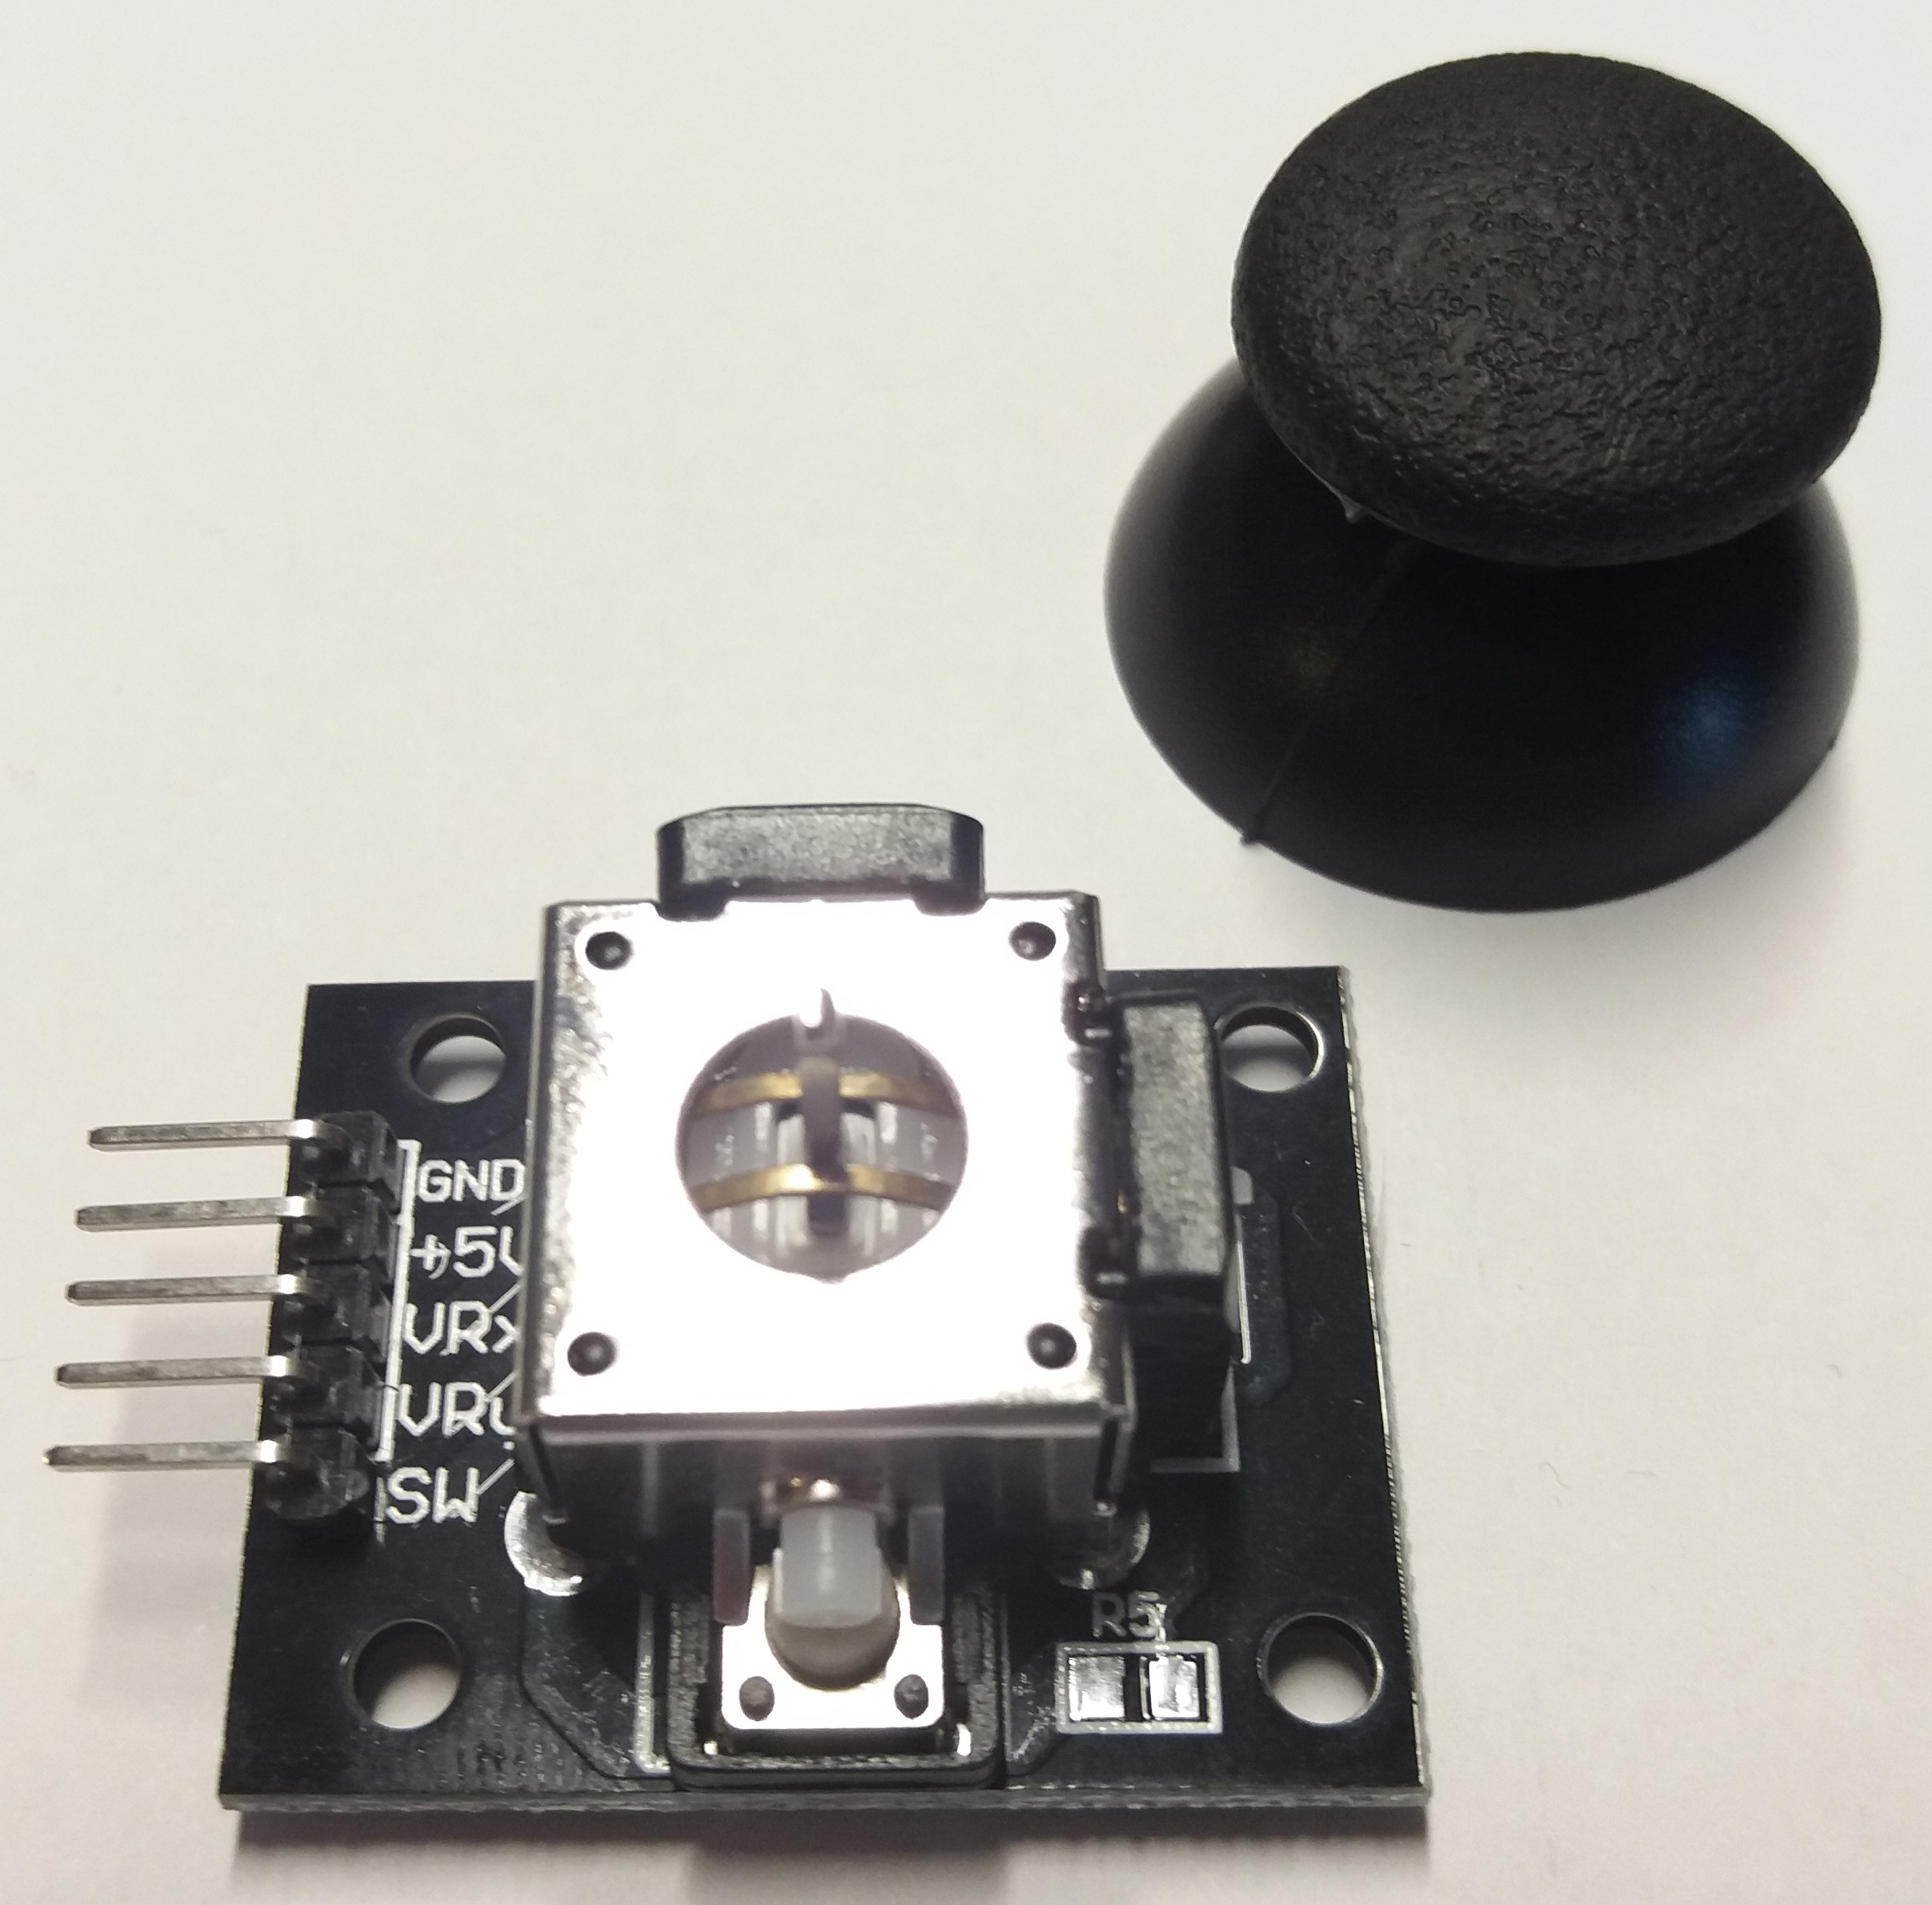
\includegraphics[width=\linewidth]{./pics/joystick.jpg}
\end{minipage}

\begin{figure}[H]
	\hfill
	\begin{minipage}{0.48\textwidth}
		\centering
		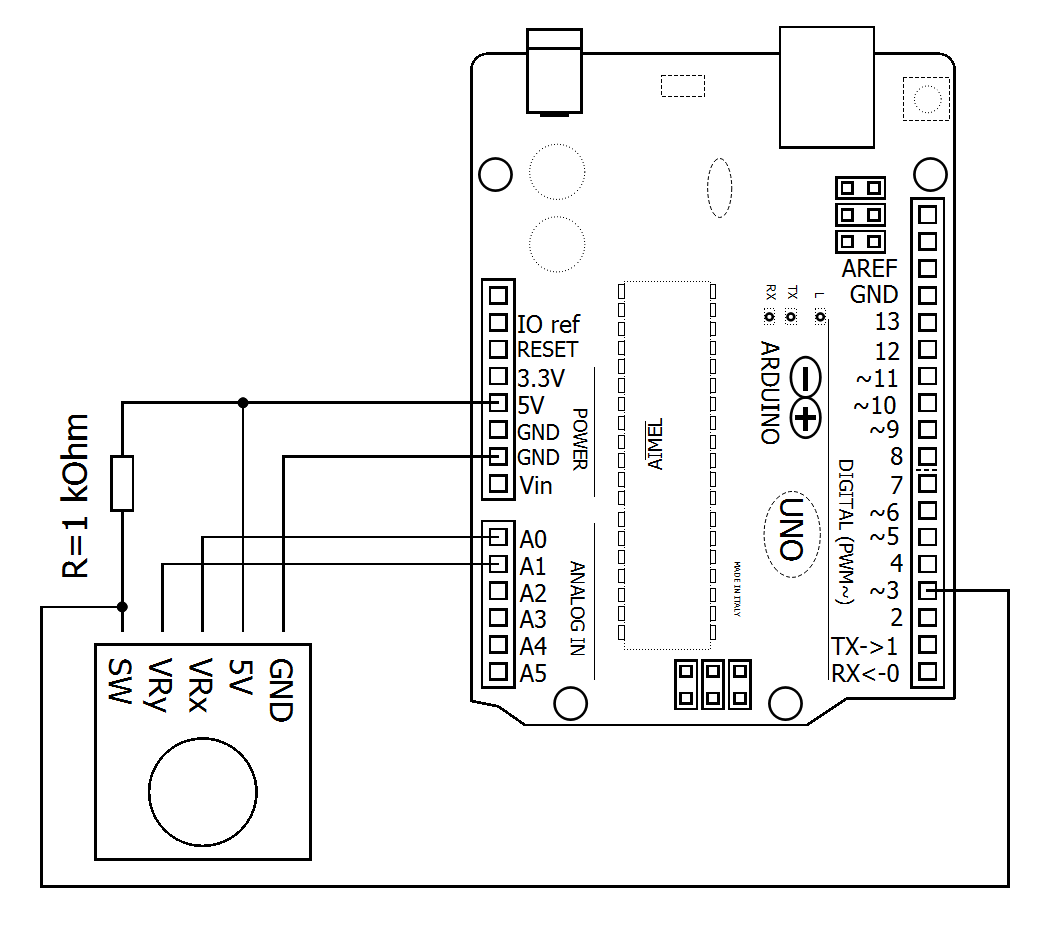
\includegraphics[width=\textwidth]{./Zeichnungen/Schaltplan-Joystick.png}
		\caption{Anschluss des Joystick-Moduls an den Arduino.}
	\end{minipage}
	\hfill
	\begin{minipage}{0.38\textwidth}
		\centering
		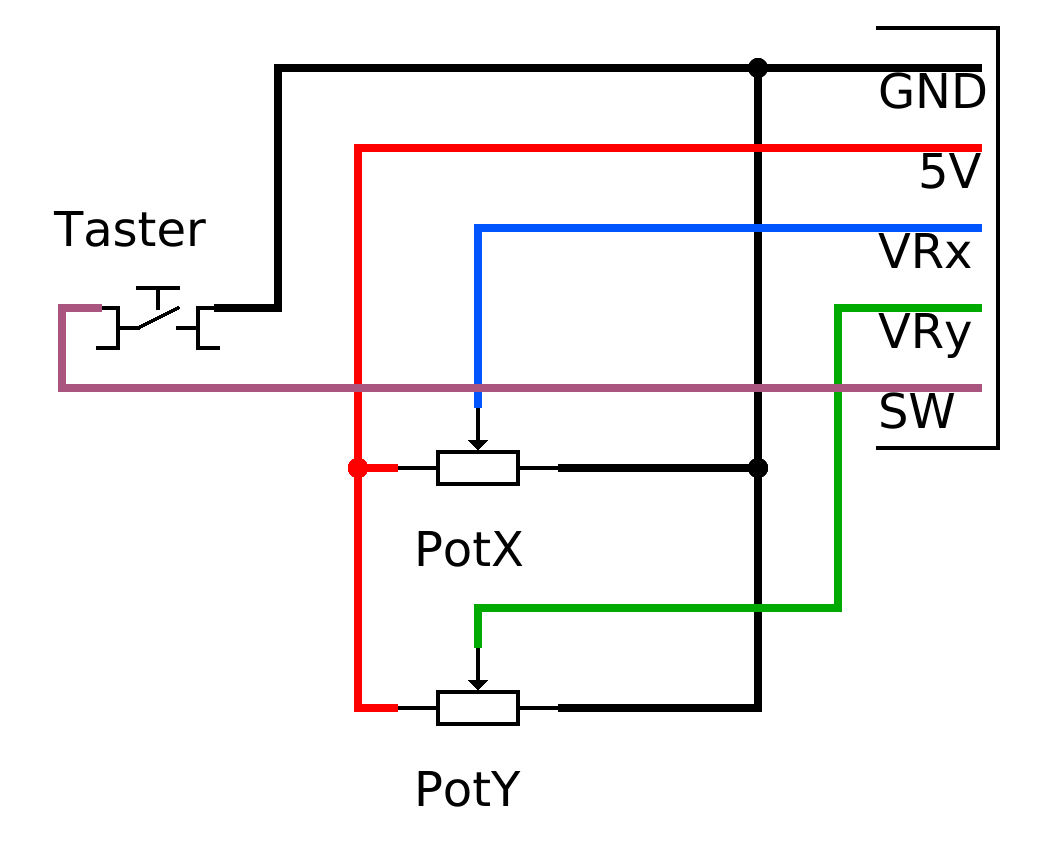
\includegraphics[width=\textwidth]{./Zeichnungen/Schaltplan-Joystick-Ersatz.png}
		\caption{Ersatzschaltplan für das Joystick-Modul.}
	\end{minipage}
	\hfill
\end{figure}

\medskip
\emph{Programmierung:} Das Joystick-Modul ist in Nepo nicht vorkonfiguriert. Die Bestandteile, also die zwei Potentiometer und der Taster, lassen sich aber einzeln konfigurieren. Dies geht wahlweise mit den vorkonfigurierten Potentiometer- und Taster-Blöcken oder als analoger und digitaler Sensor.

\medskip

\begin{aufgabe} \emph{Erste Experimente}
	\begin{enumerate}[label=\alph*), itemsep=0.5ex,parsep=0ex]
		\item Bewege den Hebel des Joystick-Moduls und beobachte, wie sich dabei die Potentiometer an den Seiten mitbewegen. Bringe auch den Plastikdeckel an, drücke den Joystick herunter und beobachte dabei das Verhalten des Tasters.
		\item Schließe das Joystick-Modul wie oben beschrieben an den Arduino an. Lies die Werte der Potentiometer aus, während du sie bewegst. Notiere, welche Bewegungsrichtung die X-Richtung und welche die Y-Richtung darstellt. Notiere außerdem, welches der beiden Potentiometer (ggü. von Taster oder ggü. der Pins) für die X-Richtung bzw. Y-Richtung verantwortlich ist.
		\item Mit dem Pullup-Widerstand wird eine sogenannte Active-Low Schaltung aufgebaut. Teste die Funktionsweise des Tasters, indem du das elektrische Potential in D3 ausliest und beschreibe, was mit dem Begriff Active-Low gemeint ist.
	\end{enumerate}
\end{aufgabe}
% El Potential an SW (Taster) schwankt ohne Pullup stark; mit Pullup wird es im offenen Fall auf 5V gezogen, im geschlossenen Fall auf 0V.
% Active-LOW: Durch Drücken wird ein 0V-Potential gelesen, also 0 oder FALSE. Das Verhalten ist genau anders herum wie man es erwarten würde.
% x-Koordinate: Veränderung durch Verschiebung in Richtung der Kabel bzw. davon weg (Poti gegenüber von Taster) (auslesen an analogem Eingang)
% y-Koordinate: Veränderung durch Verschiebung in Richtung des Tasters bzw. davon weg (Poti gegenüber der Kabel) (auslesen an analogem Eingang)

\begin{projekt}[Joystick-Motor-Steuerung]\label{proj:joystick-motor}
	Steuere mit dem Joystick-Modul einen Schrittmotor!
\end{projekt}


\textbf{Achtung bei Verwendung von Motoren:}\marginpar{\centering\ausrufezeichen} Spätestens, wenn mehr als ein Motor am Arduino betrieben werden soll, muss eine externe Spannungsquelle genutzt werden, zum Beispiel durch Anschluss einer 9\,V-Batterie an das Power-Supply-Module. Schaue dir dazu noch einmal Abschnitt \ref{sec:schrittmotor} an.

\newpage
\section{Infrarot-Sensor mit Fernbedienung}
\label{sec:infrarot-fern}

Jeder weiß, wie angenehm es ist, wenn man ein Gerät fernsteuern kann statt aufstehen zu müssen, um die angebrachten Knöpfe zu drücken. Eine einfache Möglichkeit dafür bietet eine Infrarot(IR)-Fernbedienung.

Wie am Namen zu erkennen, verwendet eine IR-Fernbedienung Infrarotstrahlen, die mit dem bloßen Auge nicht sichtbar sind. Hält man jedoch eine Digitalkamera, z.\,B. vom Smartphone, auf die Infrarot-LED der Fernbedienung und drückt eine Taste, dann kann man ein schnelles Aufblitzen erkennen. Am besten probierst du es selbst einmal aus oder schaust dir ein kurzes \video \href{https://el-voss.de/downloads/ir-strahlen.html}{Video der IR-Strahlen} an. Das Aufblitzen zeigt, dass die Strahlen in einem bestimmten Rhythmus gesendet werden, aus dem sich entschlüsseln lässt, welche Taste gedrückt wurde.

\begin{wrapfigure}{r}{0.28\textwidth}
	\centering
	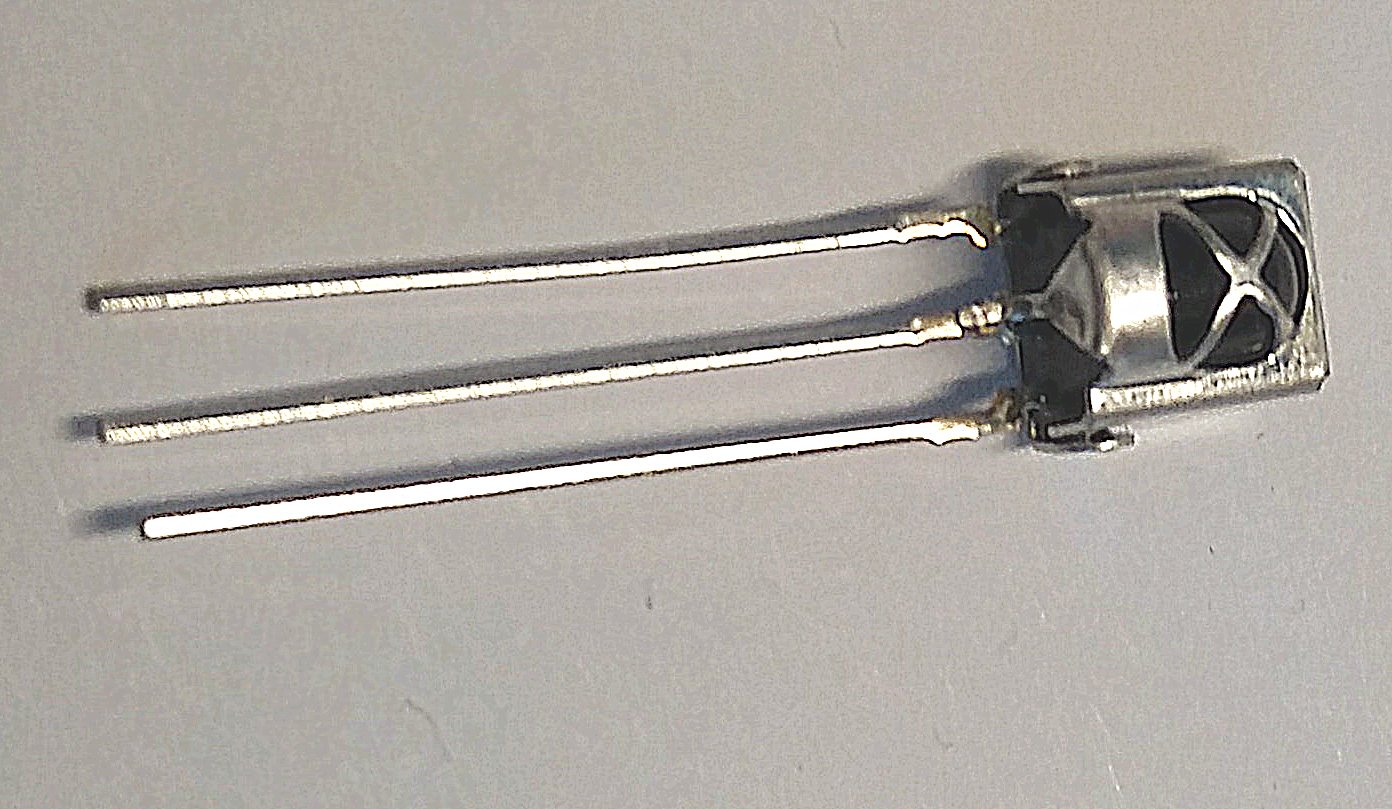
\includegraphics[width=0.24\textwidth]{./pics/ir-sensor.jpg}
	\vspace{5mm}
	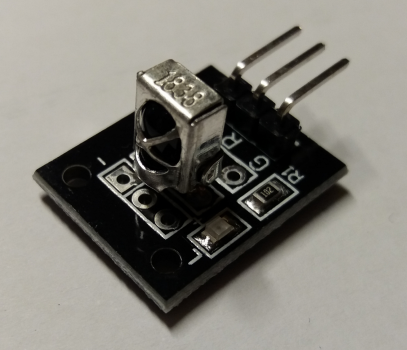
\includegraphics[width=0.24\textwidth]{./pics/ir-sensor-led-modul.png}
	\caption{Infrarotsensor (oben) und Infrarotsensor-Modul mit LED-Anzeige (unten).}
\end{wrapfigure}
Empfangen werden die Infrarotstrahlen von einem Infrarotsensor, der im Wesentlichen aus einer \href{https://de.wikipedia.org/wiki/Photodiode}{Photodiode} besteht. Diese ist sehr ähnlich wie eine Leuchtdiode aufgebaut, allerdings funktioniert sie genau umgekehrt: Anhand eintreffender (infraroter) Lichtstrahlen wird ein Stromfluss ausgelöst, der dann registriert und weiter verarbeitet werden kann. Die Photodiode reagiert zwar am empfindlichsten auf infrarotes Licht bei einer Frequenz von $\SI{38}{\kilo\hertz}$, allerdings auch (weniger stark) auf sichtbares Licht. Um dieses sichtbare Licht, insbesondere die Umgebungshelligkeit, wegzufiltern, befindet sich die Photodiode in einer schwarzen Kunstharzschicht. 

Häufig wird der Infrarotsensor zusammen mit einer LED und einem zugehörigen Vorwiderstand auf einer kleinen Platine ausgeliefert, damit das Empfangen eines Signals durch die LED angezeigt werden kann. Es sind aber auch Infrarotsensoren ohne weitere Anzeige im Umlauf.

%\medskip
%\begin{minipage}{0.7\textwidth}
%	Empfangen werden die Infrarotstrahlen von einem Infrarotsensor, der im Wesentlichen aus einer \href{https://de.wikipedia.org/wiki/Photodiode}{Photodiode} besteht. Diese ist sehr ähnlich wie eine Leuchtdiode aufgebaut, allerdings funktioniert sie genau umgekehrt: Anhand eintreffender (infraroter) Lichtstrahlen wird ein Stromfluss ausgelöst, der dann registriert und weiter verarbeitet werden kann. Die Photodiode reagiert zwar am empfindlichsten auf infrarotes Licht bei einer Frequenz von $\SI{38}{\kilo\hertz}$, allerdings auch (weniger stark) auf sichtbares Licht. Um dieses sichtbare Licht, insbesondere die Umgebungshelligkeit, wegzufiltern, befindet sich die Photodiode in einer schwarzen Kunstharzschicht. 
%	
%	Häufig wird der Infrarotsensor zusammen mit einer LED und einem zugehörigen Vorwiderstand auf einer kleinen Platine ausgeliefert, damit das Empfangen eines Signals durch die LED angezeigt werden kann. Es sind aber auch Infrarotsensoren ohne weitere Anzeige im Umlauf.
%	
%	Der Anschluss an den Arduino ist einfach: GND und 5V dienen wie üblich der Stromversorgung. Der Signal-Pin S muss mit einem beliebigen PWM-Pin (mit $\sim$) verbunden werden. Die Pin-Belegung ist aber leider unterschiedlich; je nach dem, ob man ein Modul mit LED-Anzeige oder nur den Infrarotsensor anschließt.
%\end{minipage}
%\hfill
%\begin{minipage}{0.28\textwidth}
%	\begin{figure}[H]
%		\centering
%		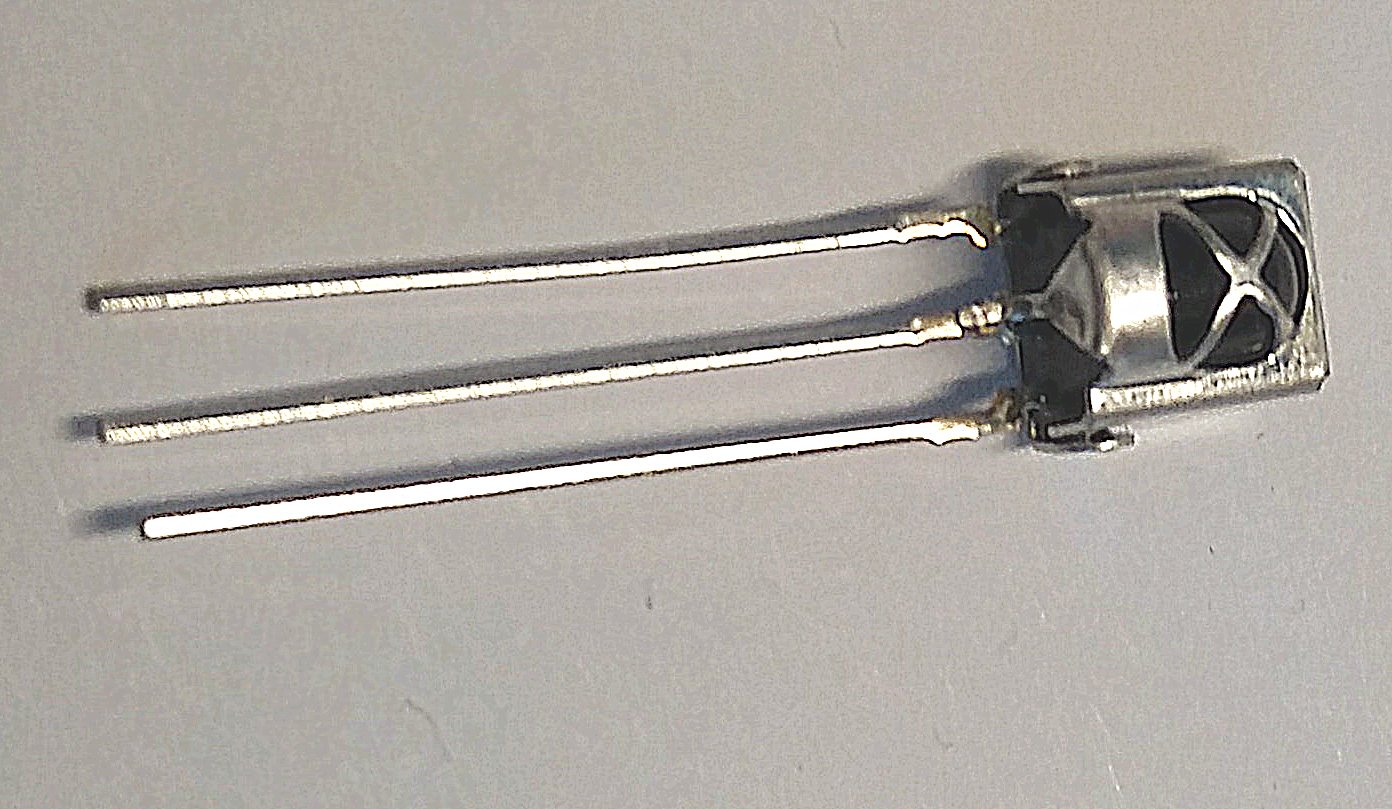
\includegraphics[width=0.7\textwidth]{./pics/ir-sensor.jpg}
%		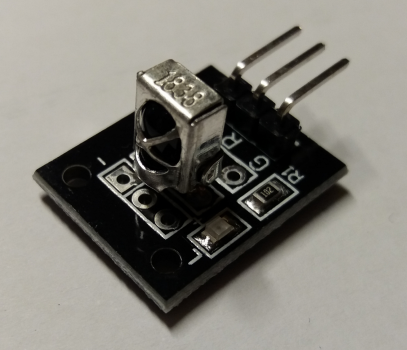
\includegraphics[width=0.7\textwidth]{./pics/ir-sensor-led-modul.png}
%		\caption{Infrarotsensor (oben) und Infrarotsensor-Modul mit LED-Anzeige (unten).}
%	\end{figure}	
%\end{minipage}
\medskip

\begin{minipage}{0.48\textwidth}
	\begin{figure}[H]
		\centering
		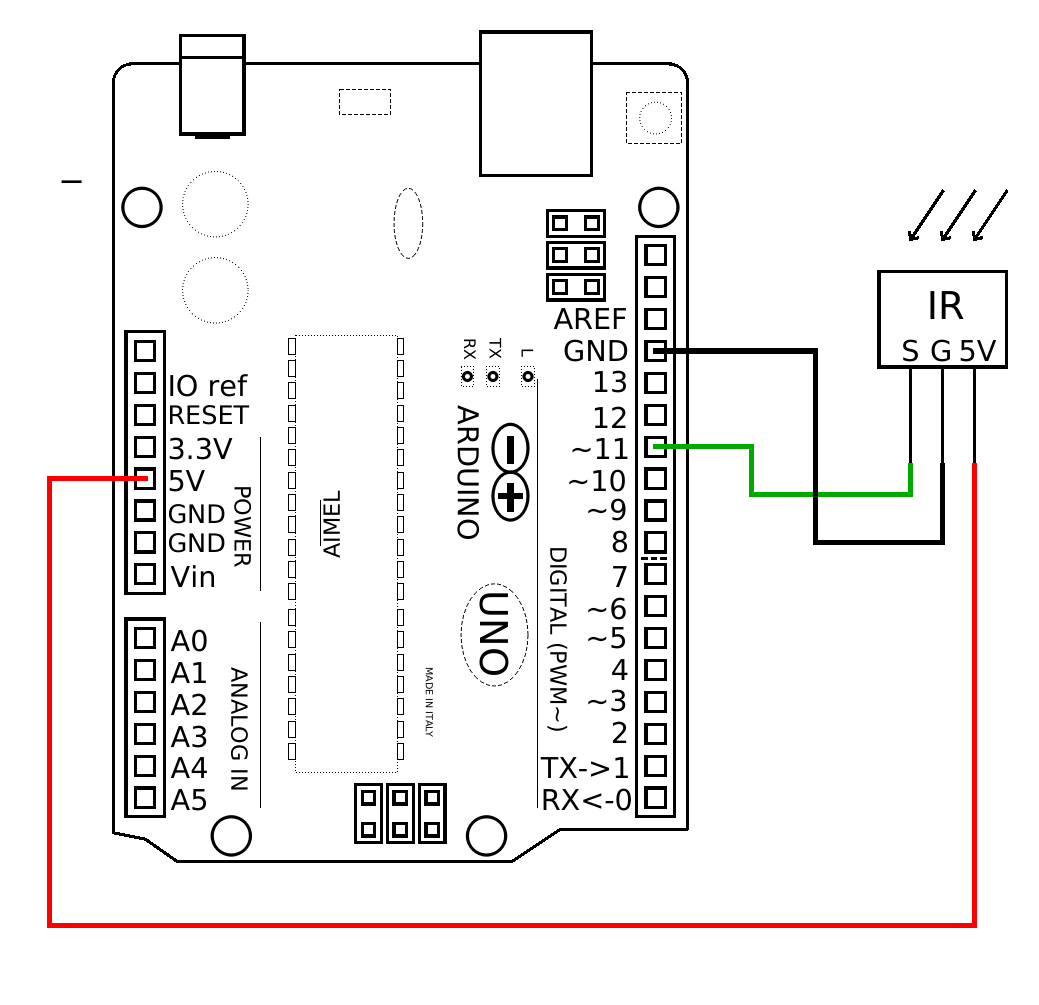
\includegraphics[width=0.8\textwidth]{./Zeichnungen/schaltplan-ir-sensor.png}
		\caption{Schaltplan zum Anschluss eines Infrarotsensors am Arduino.}
	\end{figure}
\end{minipage}
\hfill
\begin{minipage}{0.48\textwidth}
	\begin{figure}[H]
		\centering
		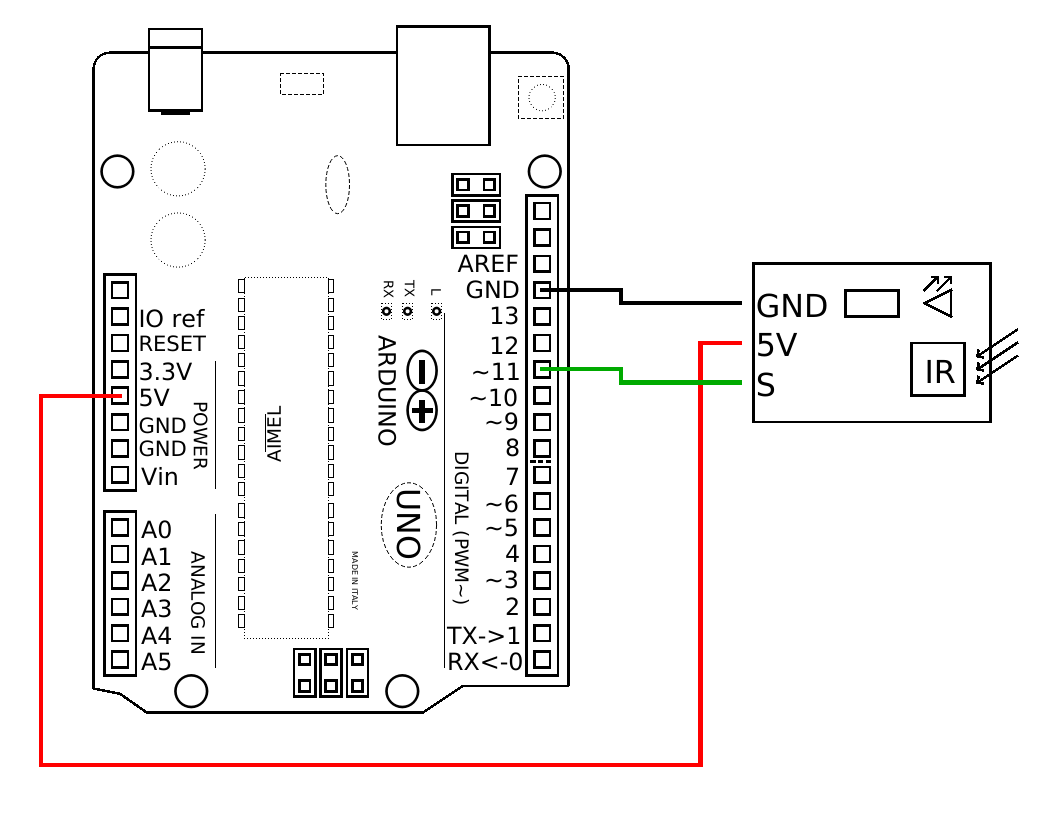
\includegraphics[width=0.95\textwidth]{./Zeichnungen/schaltplan-ir-sensor-modul.png}
		\caption{Schaltplan zum Anschluss eines Infrarotsensormoduls mit LED-Anzeige am Arduino.}
	\end{figure}
\end{minipage}
\medskip

Der Anschluss an den Arduino ist einfach: GND und 5V dienen wie üblich der Stromversorgung. Der Signal-Pin S muss mit einem beliebigen PWM-Pin (mit $\sim$) verbunden werden. Die Pin-Belegung ist aber leider unterschiedlich; je nach dem, ob man ein Modul mit LED-Anzeige oder nur den Infrarotsensor anschließt.

Nachdem der IR-Sensor mit dem Arduino verbunden und in Nepo konfiguriert wurde, können die empfangenen Werte in Nepo abgefragt werden. Abbildung \ref{abb:ir-fernbedienung-auslesen} zeigt ein einfaches Beispiel, wie mit den Tasten 0 und 1 auf einer Infrarot-Fernbedienung die Board-LED des Arduino an- und ausgestellt werden kann. Wenn die Taste mehrere Aktionen auslösen soll (wie die Ausgabe des Codes auf dem seriellen Monitor und das Anschalten der LED), dann muss der Wert in einer Variable gespeichert werden.

\begin{figure}[H]
	\centering
	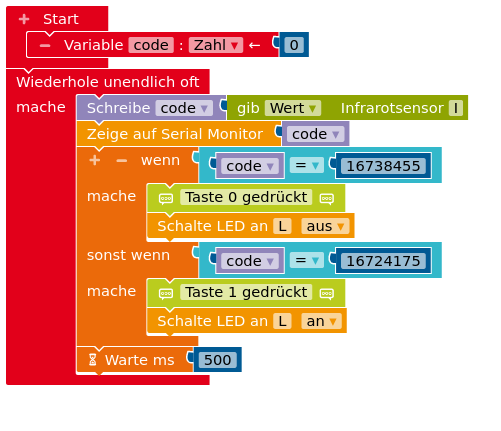
\includegraphics[width=0.6\textwidth]{./pics/ir-fernbedienung-auslesen.png}
	\caption{Einfaches Beispielprogramm zur Verwendung einer IR-Fernbedienung.}
	\label{abb:ir-fernbedienung-auslesen}
\end{figure}

\begin{aufgabe} \emph{Codes kennen lernen}
	\begin{enumerate}[label=\alph*),itemsep=0mm,parsep=0mm]
		\item Übertrage das oben abgebildete Programm auf den Arduino und probiere es aus.
		\item Erstelle eine Tabelle, in der du den Zahlencode für jede Taste festhälst. Probiere auch aus, was passiert, wenn du die Tasten länger gedrückt hälst.
	\end{enumerate}
\end{aufgabe}

\marginpar{%
	\footnotesize%
	\video \\
	\href{https://www.youtube.com/watch?v=1PUyE8QJuAw}{Lichterkette-Beispielvideo}
}
\begin{projekt}[Fernsteuerung eines LED-Streifens]\label{proj:fernsteuerung-lauflicht}
	In vielen Bereichen werden LED-Streifen genutzt, um einen Raum mit passendem, indirektem Licht auszustatten. Die meisten LED-Streifen lassen sich über eine kleine Infrarot-Fernbedienung steuern, wodurch sich die Farbe, aber auch der Modus einstellen lässt - zum Beispiel eine einzelne Farbe, \hyperref[sec:pwm]{Fading}, Strobe, \dots
	
	Das Prinzip lässt sich auf ein Lauflicht übertragen. Baue ein Lauflicht und programmiere verschiedene Lauflicht-Modi, die sich mit der Fernbedienung einstellen lassen.
\end{projekt}


\newpage
\section{Temperatur- und Luftfeuchtigkeitssensor DHT-11}
\label{sec:templuft}

\begin{minipage}{0.7\textwidth}
	Bei vielen Umweltmessungen interessiert nicht nur die Temperatur, sondern auch die Luftfeuchtigkeit. Der Sensor DHT-11 ist ein einfaches, kleines Bauteil, mit dem sich beides messen lässt.
	
\end{minipage}
\hfill
\begin{minipage}{0.25\textwidth}
	\centering
	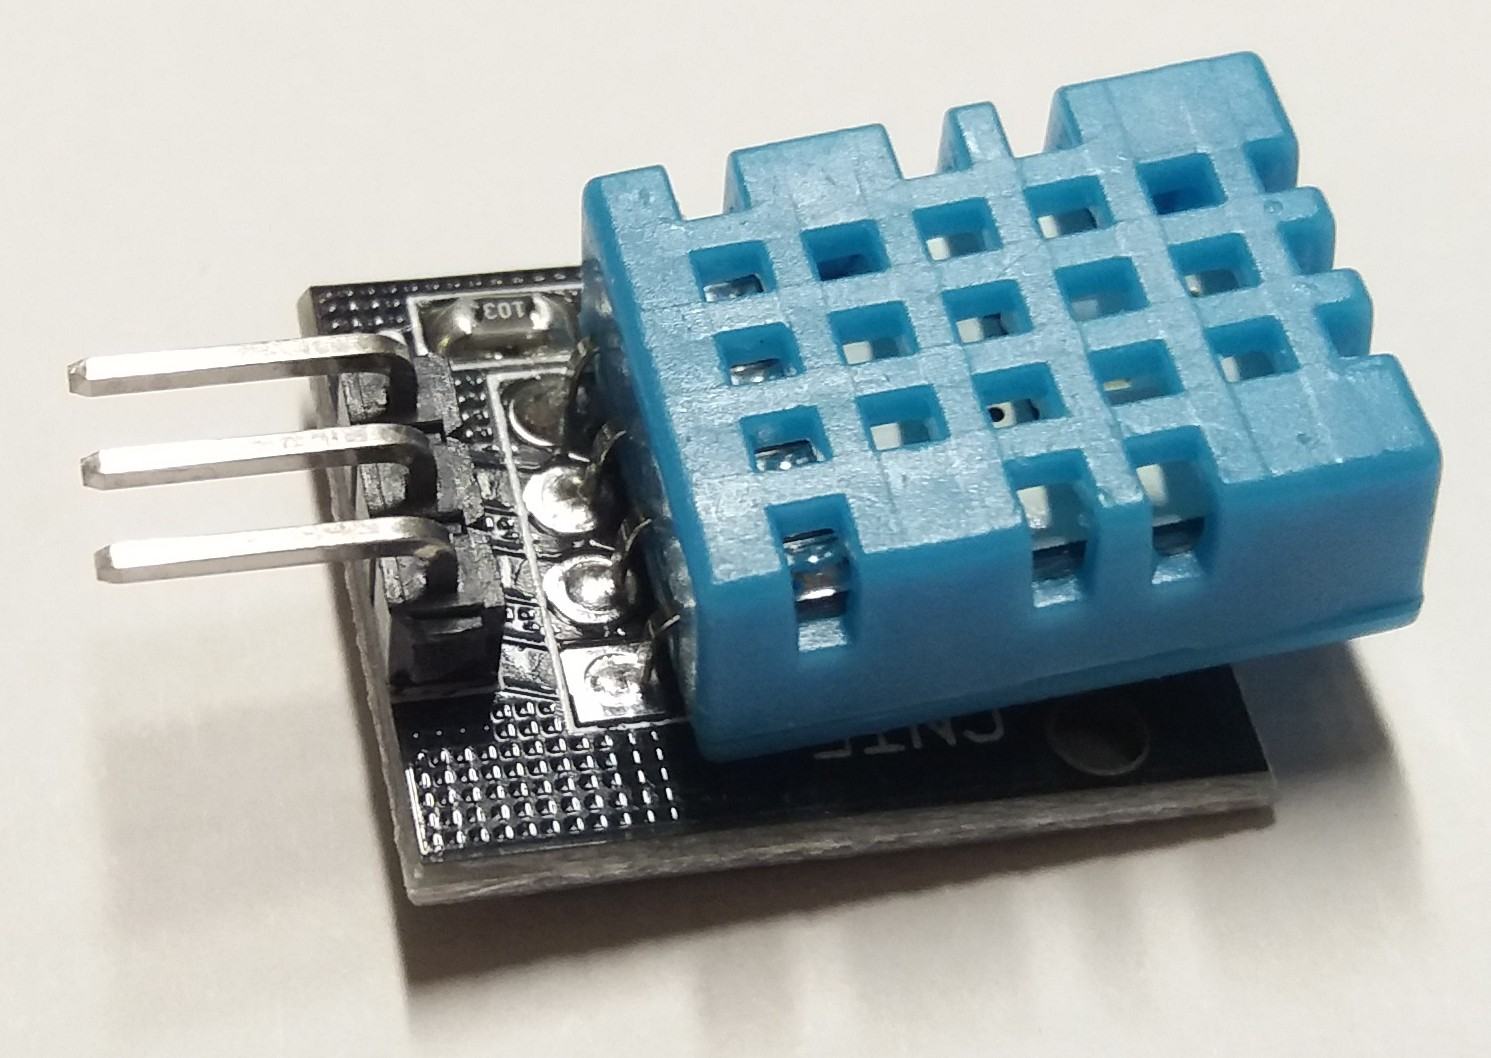
\includegraphics[width=0.84\textwidth]{./pics/dht11.jpg}
\end{minipage}
\medskip

Der DHT-11 verfügt über drei Pins - 5V und GND dienen der Stromversorgung, während das Signal zu den Messdaten über den Signalpin ausgegeben wird. Für die Temperaturmessung ist auf dem DHT-11 ein NTC verbaut.

\begin{figure}[H]
	\centering
	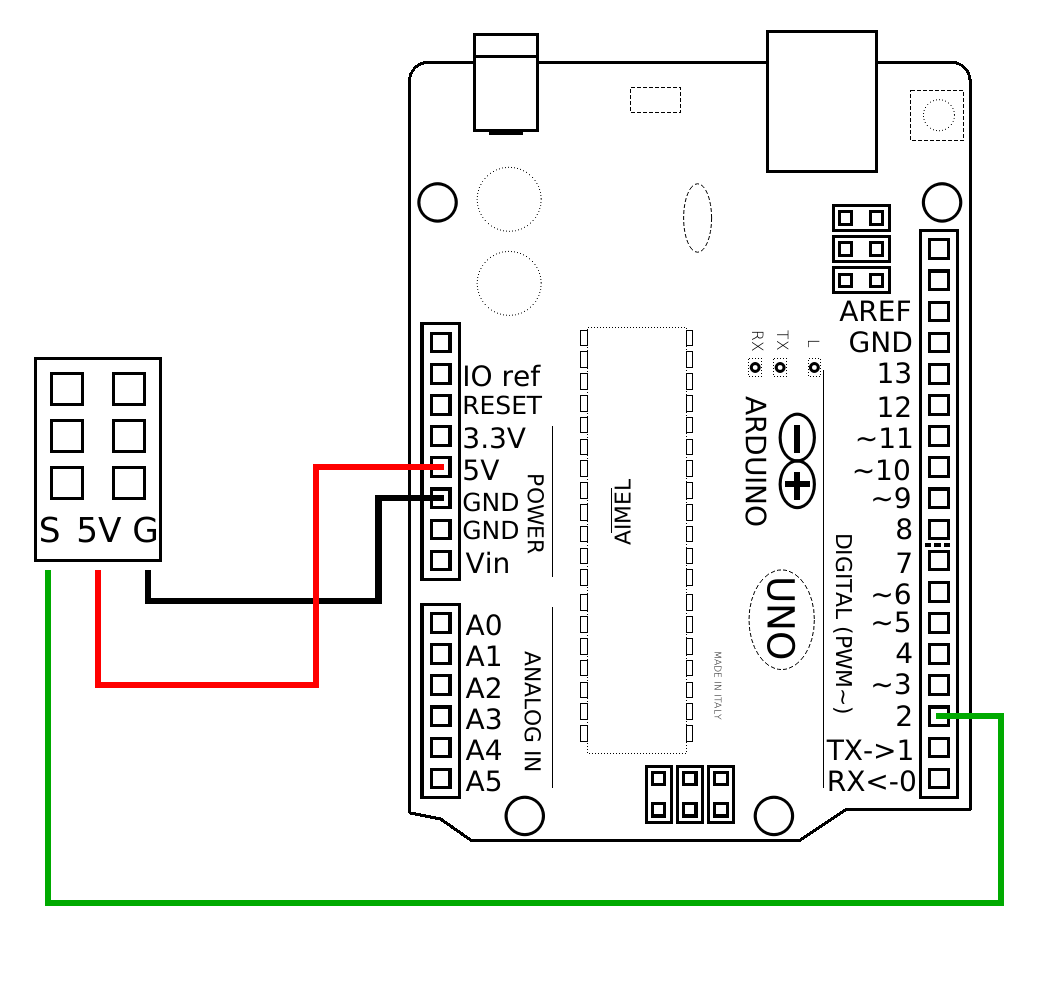
\includegraphics[width=0.4\textwidth]{./Zeichnungen/Schaltplan-DHT11.png}
\end{figure}

\vspace{-\baselineskip}
\begin{wrapfigure}{r}{0.5\textwidth}
	\centering
	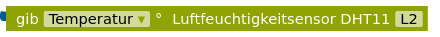
\includegraphics[width=0.5\textwidth]{./pics/dht-gibTemperatur.png}
	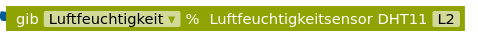
\includegraphics[width=0.5\textwidth]{./pics/dht-gibLuftfeuchtigkeit.png}
\end{wrapfigure}
Das Auslesen des Signalpins ist einfach, weil der DHT-11 in der Konfiguration bereits implementiert wurde, sodass man nur noch den Signalpin angeben muss. Das Signal wird dann automatisch analysiert und decodiert, um anhand der entsprechenden Befehle auf die übermittelte Temperatur bzw. Luftfeuchtigkeit zuzugreifen. Die Größe kann über das Drop-Down-Menü ausgewählt werden.

\bigskip
\begin{projekt}[Wetterstation]\label{proj:wetterstation}
	Baue eine kleine Wetterstation, die alle zehn Minuten Temperatur und Luftfeuchtigkeit misst und auf dem seriellen Monitor ausgibt.
\end{projekt}
% Wetterstation
%Badezimmerlüfter

\begin{recherche}{Wie wird die Luftfeuchtigkeit gemessen?}
	Mit dem DHT-11 lässt sich die relative Luftfeuchtigkeit bestimmen. Recherchiere, was darunter zu verstehen ist, und wie diese durch ein elektrisches Bauteil gemessen wird.
\end{recherche}

\newpage
\section{Temperatursensor TMP36}
\label{sec:tmp36}

\begin{minipage}{0.58\textwidth}
	Bei deinen Temperaturmessungen mit einem NTC oder dem DHT-11 (in dem auch ein NTC verbaut ist), hast du vielleicht festgestellt, dass die Bauteile nicht besonders genau arbeiten. Für professionellere Anwendungen benötigt man eine wesentlich höhere Genauigkeit. Hier kann der TMP36 helfen: Er hat eine Genauigkeit von $\pm \SI{1}{\celsius}$ und kann Temperaturen in einem Bereich von $\SI{-40}{\celsius}$ bis $\SI{125}{\celsius}$ zuverlässig messen. Die Messung der Temperatur erfolgt über die Messung einer temperaturabhängigen Spannung. Bei $\SI{0}{\celsius}$ beträgt die Spannung $\SI{500}{\milli\volt}$ (ein sogenannter \emph{Offset}).
\end{minipage}
\hfill
\begin{minipage}{0.4\textwidth}
	\begin{figure}[H]
		\begin{minipage}{0.48\textwidth}
			\centering
			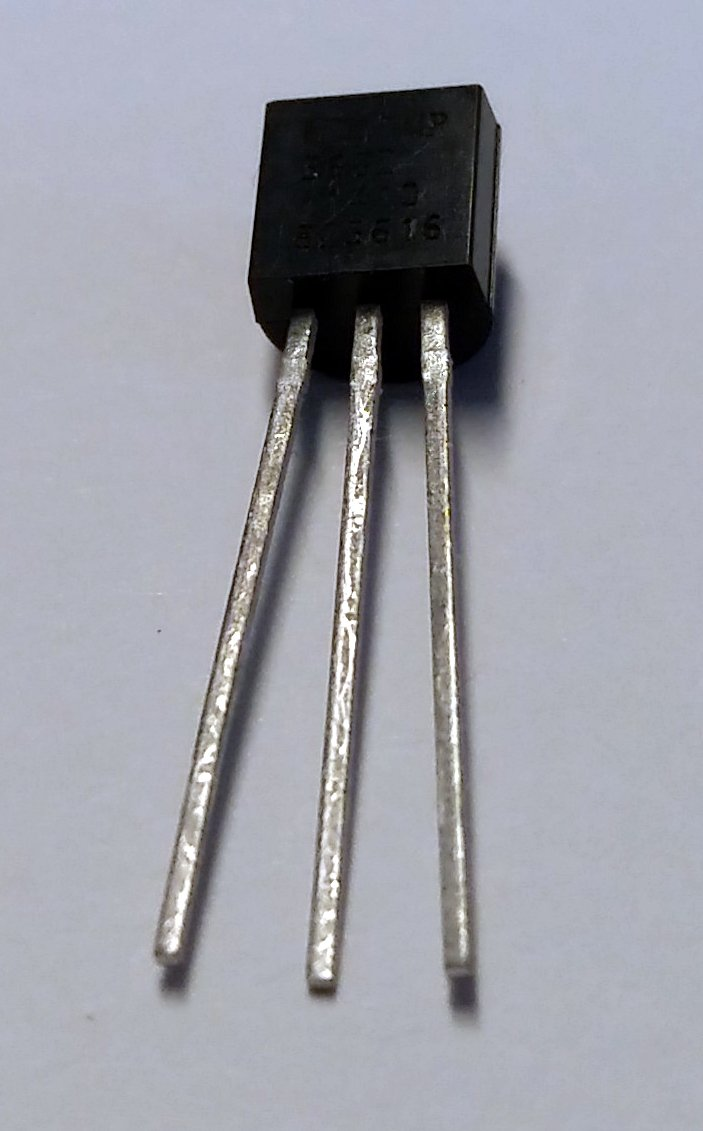
\includegraphics[width=0.8\textwidth]{./pics/tmp36.jpg}
		\end{minipage}
		\hfill
		\begin{minipage}{0.48\textwidth}
			\centering
			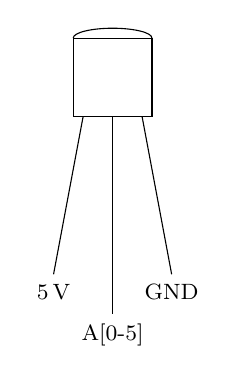
\begin{tikzpicture}[scale=2.5]
			\draw (-0.2,0.8) rectangle (0.2,1.2);
			\draw (0.2,1.2) arc [start angle=0,end angle=180,x radius=0.2,y radius=0.05];
			\draw (-0.15,0.8) -- (-0.3,0) node [below] {\footnotesize 5\,V};
			\draw (0,0.8) -- (0,-0.2) node [below] {\footnotesize A[0-5]};
			\draw (0.15,0.8) -- (0.3,0) node [below] {\footnotesize GND};
			\end{tikzpicture}
		\end{minipage}
		\caption{Temperatursensor TMP36 (links) mit Pinbelegung (rechts, Blick auf flache Seite). \\
		\textbf{Achtung:} Verwechslungsgefahr mit Transistor (Aufschrift beachten)!}
	\end{figure}
	\medskip
	
\end{minipage}
\smallskip

Ein weiterer Vorteil des TMP36 ist, dass die Abhängigkeit von ausgegebener Spannung und Temperatur linear verläuft: Eine Temperaturänderung von $\SI{1}{\celsius}$ entspricht immer einer Spannungsänderung von $\SI{10}{\milli\volt}$.

\begin{aufgabe} \emph{Vergleich von Kennlinien}
	
	Ein linearer Zusammenhang zwischen der gemessenen Größe (oft eine Spannung) und der gesuchten Größe (hier die Temperatur) gilt als vorteilhaft, ein exponentieller Zusammenhang dagegen als nachteilig. Begründe anhand der unten abgebildeten Skizzen von Kennlinien, warum ein linearer Zusammenhang besser ist.
	
	\emph{Beachte: Jede Messung ist mit einem Fehler versehen!} 
\end{aufgabe}

\begin{minipage}{0.48\textwidth}
	\begin{figure}[H]
		\centering
		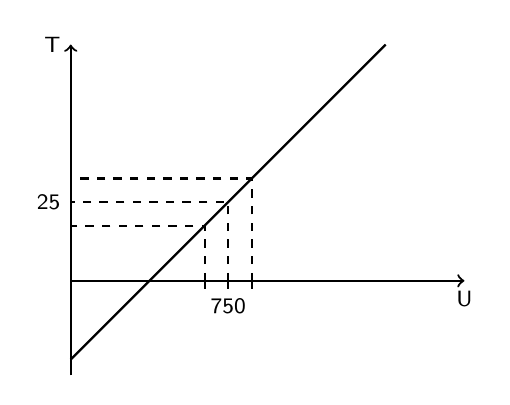
\begin{tikzpicture}[thick]
			% Koordinatensystem und Funktion
			\draw [->] (0,-1.2) -- (0,3) node [left] {\sffamily \footnotesize T};
			\draw [->] (0,0) -- (5,0) node [below] {\sffamily \footnotesize U};
			\draw [domain=0:4] plot (\x, {-1+\x});
			% Zahlen und Verbindung
			\draw (2,0.1) -- (2,-0.1) node [below] {\sffamily \footnotesize 750};
			\draw [dashed] (2,0) -- (2, -1+2) -- (0,-1+2) node [left] {\sffamily \footnotesize 25};
			% Fehlerticks und Verbindungen
			\draw (1.7, 0.1) -- (1.7, -0.1);
			\draw [dashed] (1.7,0) -- (1.7, -1+1.7) -- (0,-1+1.7);
			\draw (2.3, 0.1) -- (2.3, -0.1);
			\draw [dashed] (2.3,0) -- (2.3, -1+2.3) -- (0,-1+2.3);
		\end{tikzpicture}
		\caption{Lineare Kennlinie.}
	\end{figure}
\end{minipage}
\hfill
\begin{minipage}{0.48\textwidth}
	\begin{figure}[H]
		\centering
		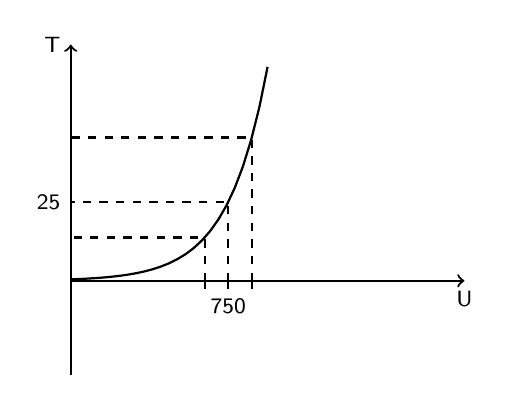
\begin{tikzpicture}[thick]
		% Koordinatensystem und Funktion
		\draw [->] (0,-1.2) -- (0,3) node [left] {\sffamily \footnotesize T};
		\draw [->] (0,0) -- (5,0) node [below] {\sffamily \footnotesize U};
		\draw [domain=0:2.5] plot (\x, {exp(2*(\x-2)});
		% Zahlen und Verbindung
		\draw (2,0.1) -- (2,-0.1) node [below] {\sffamily \footnotesize 750};
		\draw [dashed] (2,0) -- (2, 1) -- (0,1) node [left] {\sffamily \footnotesize 25};
		% Fehlerticks und Verbindungen
		\draw (1.7, 0.1) -- (1.7, -0.1);
		\draw [dashed] (1.7,0) -- (1.7, 0.55) -- (0,0.55);
		\draw (2.3, 0.1) -- (2.3, -0.1);
		\draw [dashed] (2.3,0) -- (2.3, 1.82) -- (0,1.82);
		\end{tikzpicture}
		\caption{Exponentielle Kennlinie.}
	\end{figure}
\end{minipage}

\medskip
\begin{projekt}[Präzises Thermometer]\label{proj:praezisesthermometer}
	\vspace{-0.5\baselineskip}
	\begin{enumerate}[label=\alph*), itemsep=0ex, parsep=0ex]
		\item Baue ein präzises Thermometer mit den vorkonfigurierten Nepo-Blöcken für den TMP36.
		\item Baue ein präzises Thermometer und konfiguriere den TMP36 als analogen Sensor.
		
		\emph{Tipp:} Zur Berechnung der Temperatur musst du zuerst den eingelesenen Analogwert in eine Spannung umrechnen. Um aus der Spannung die Temperatur zu berechnen, musst du die oben angegebenen Informationen noch einmal genau lesen. Zur Kontrolle: Die maximal mögliche Spannung am Signalpin beträgt $\SI{2}{\volt}$, was einer Temperatur von $\SI{150}{\celsius}$ entspricht.
	\end{enumerate}
\end{projekt}

\newpage
\section{Tropfensensor und Feuchtigkeitssensor}
\label{sec:tropfensensor}

\begin{wrapfigure}{r}{0.4\textwidth}
	\centering
	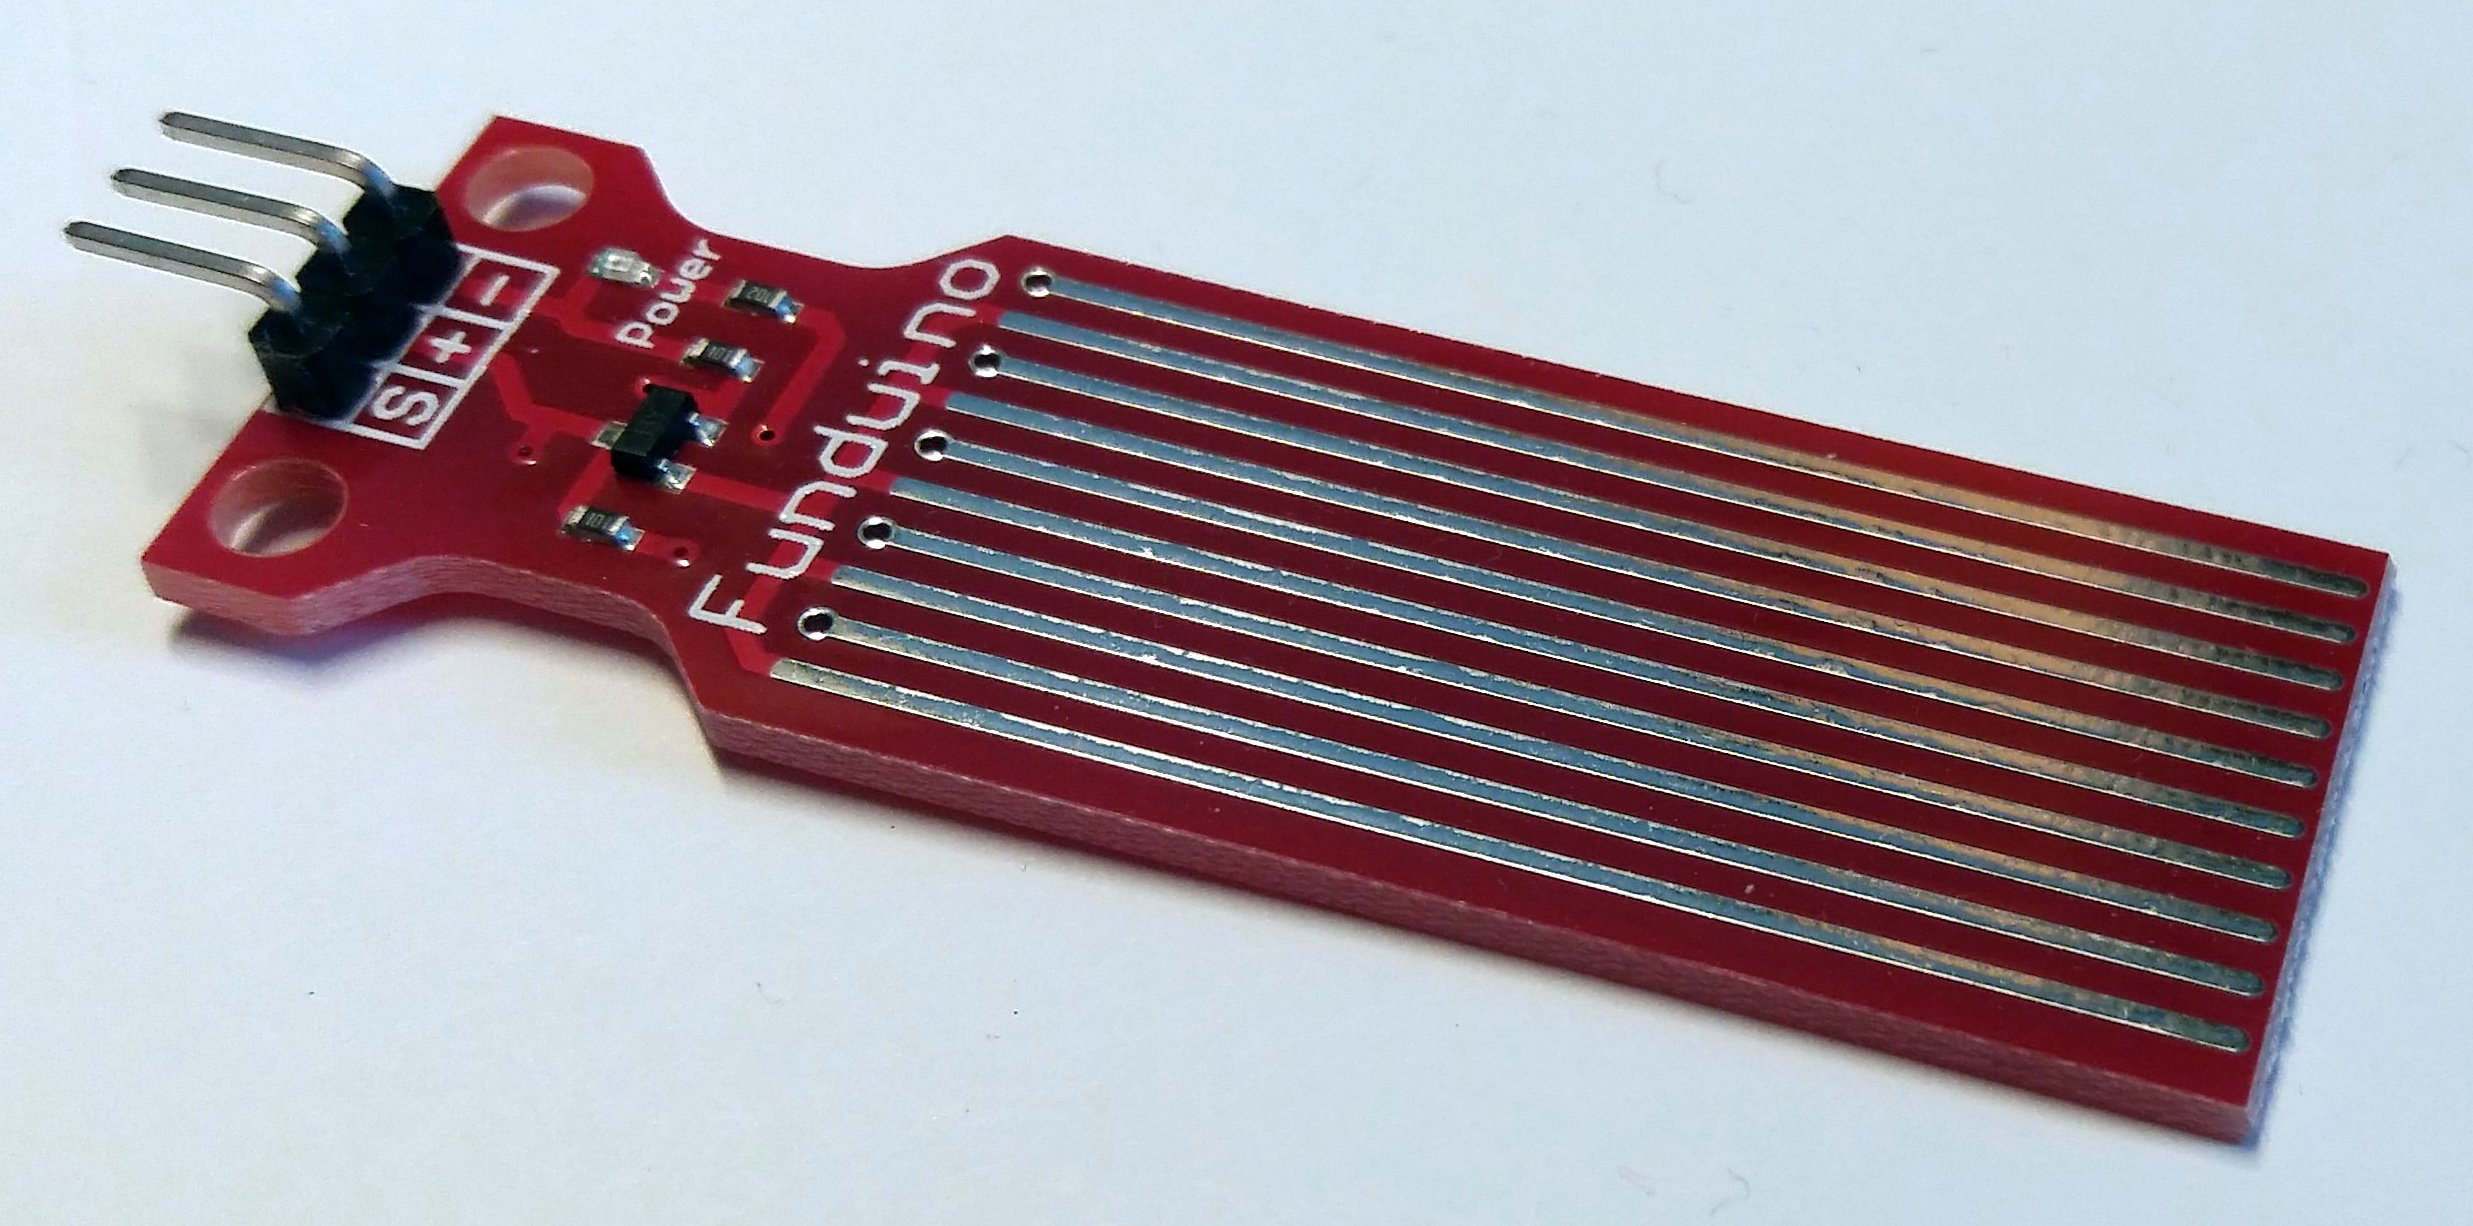
\includegraphics[width=0.35\textwidth]{./pics/tropfensensor.jpg}
	
	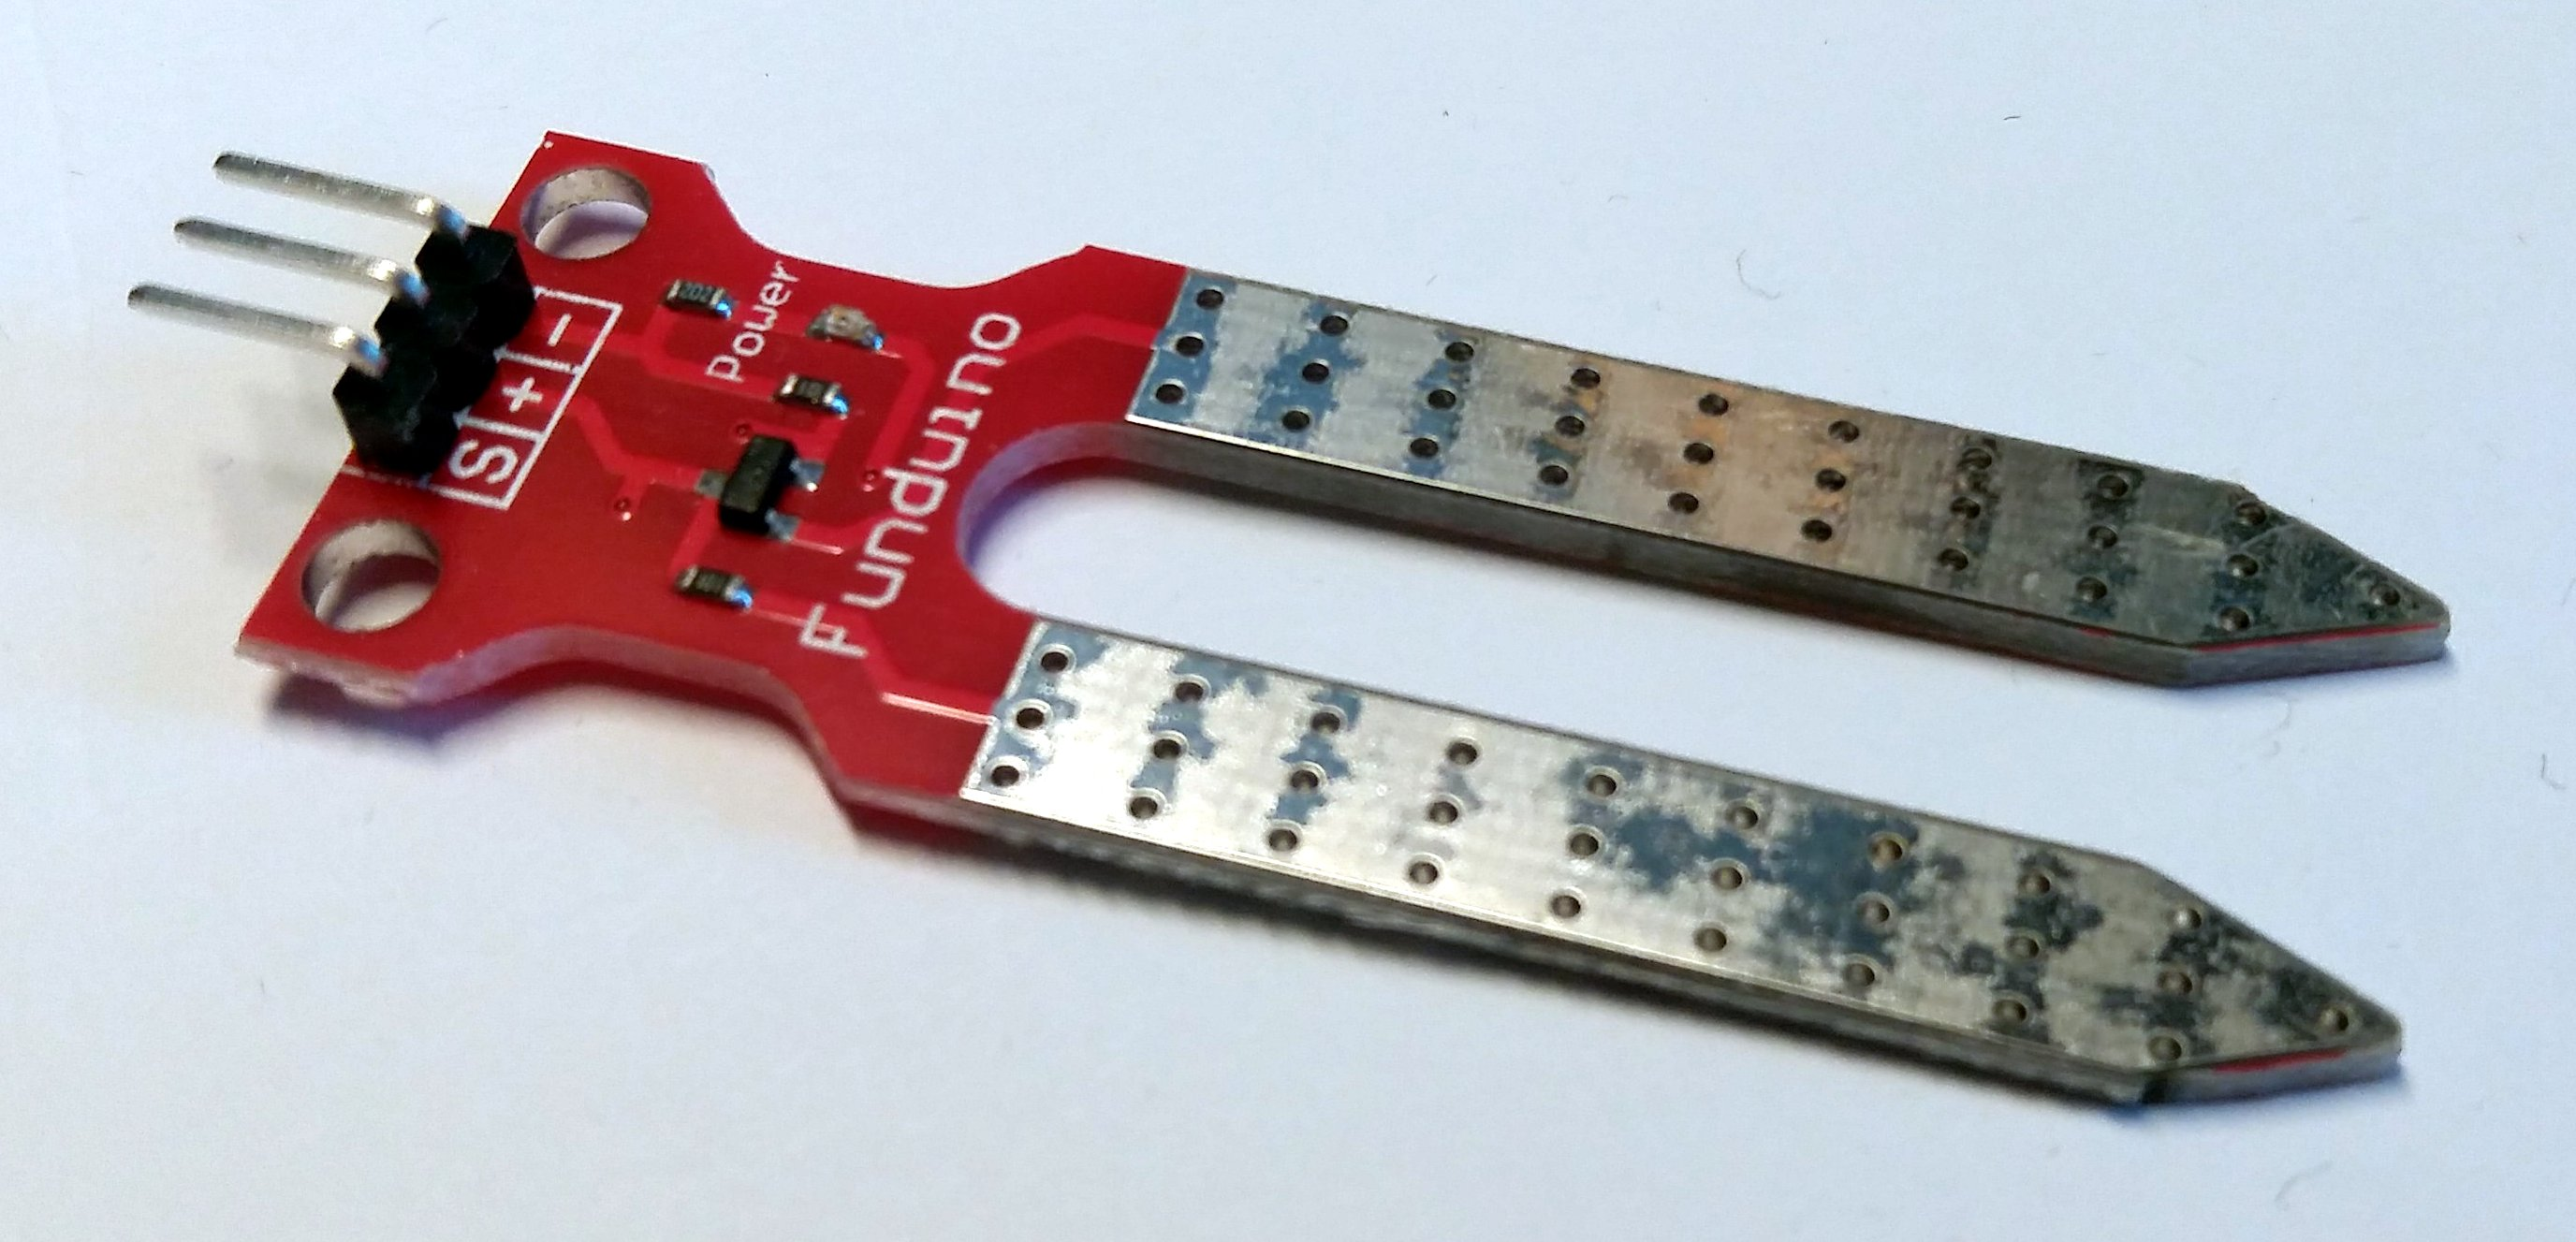
\includegraphics[width=0.35\textwidth]{./pics/feuchtigkeitssensor.jpg}
	\caption{Tropfensensor (oben) und Feuchtigkeitssensor (unten). Anschluss am Arduino: \\S > A[0-5] \qquad + > 5\,V \qquad - > GND.}
\end{wrapfigure}
Mit einem Tropfensensor lässt sich die Feuchtigkeit auf dem Sensorblatt messen. Solche Sensoren werden zum Beispiel in Windschutzscheiben von Autos eingesetzt, um die Scheibenwischer und ihre Geschwindigkeit zu steuern. Feuchtigkeitssensoren funktionieren im Wesentlichen genauso, allerdings sind die Kontakte dabei so weit auseinander, dass durch Tropfen noch kein Stromfluss entsteht, sondern erst durch zum Beispiel die feuchte Erde eines Blumentopfes, der automatisch bewässert werden soll.

Der Anschluss an den Arduino ist in beiden Fällen einfach (siehe rechts). Am Signalpin wird eine Spannung (als Analogwert im analogen Eingang) gemessen, die im trockenen Zustand bei $\SI{0}{\volt}$ (0) liegt und bis zu $\SI{5}{\volt}$ (1023) steigen kann.

\begin{aufgabe} \emph{Theorie: Wie kann man Feuchtigkeit messen?}
	
	Das grundlegende Prinzip eines Tropfensensors/Feuchtigkeitssensors ist einfach: Je nasser/feuchter es ist, desto besser der Strom durch die feuchte Stelle fließen. Der Arduino kann aber nur eine Spannung messen (als Analogwert) - wie bekommt man diese Umwandlung hin?
	
	Erkläre anhand des unten abgebildeten Schaltplans eines Tropfensensors, wie die Feuchtigkeit auf den Kontakten des Sensorblatts am Signalpin S (analoger Eingang zur Spannungsmessung) gemessen werden kann.
	
	\emph{Tipp:} Zentral ist der Transistor J3Y, der mit seinen drei Kontakten auf dem Sensor gut erkennbar ist. Die Status-LED mit Vorwiderstand kann dagegen vernachlässigt werden.
\end{aufgabe}
\marginpar{%
	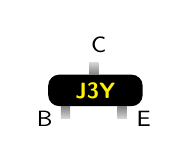
\begin{tikzpicture}[scale=0.4]
	\fill[black, rounded corners] (0,0) rectangle (3,1);
	\node at (1.5,0.5) {\color{yellow}\sffamily\bfseries\footnotesize J3Y};
	\shade [bottom color=gray!30, top color=gray] (0.4,0) rectangle ++(0.3,-0.4) node [left=1mm] {\sffamily\footnotesize B};
	\shade [bottom color=gray!30, top color=gray] (2.2,0) rectangle ++(0.3,-0.4) node [right] {\sffamily\footnotesize E};
	\shade [bottom color=gray, top color=gray!30] (1.3,1) rectangle ++(0.3,0.4) node [above] {\sffamily\footnotesize C};
	\end{tikzpicture}
	\scriptsize Pinbelegung des Transistors J3Y auf dem Tropfen- und Feuchtigkeitssensor.
}
\begin{figure}[H]
	\centering
	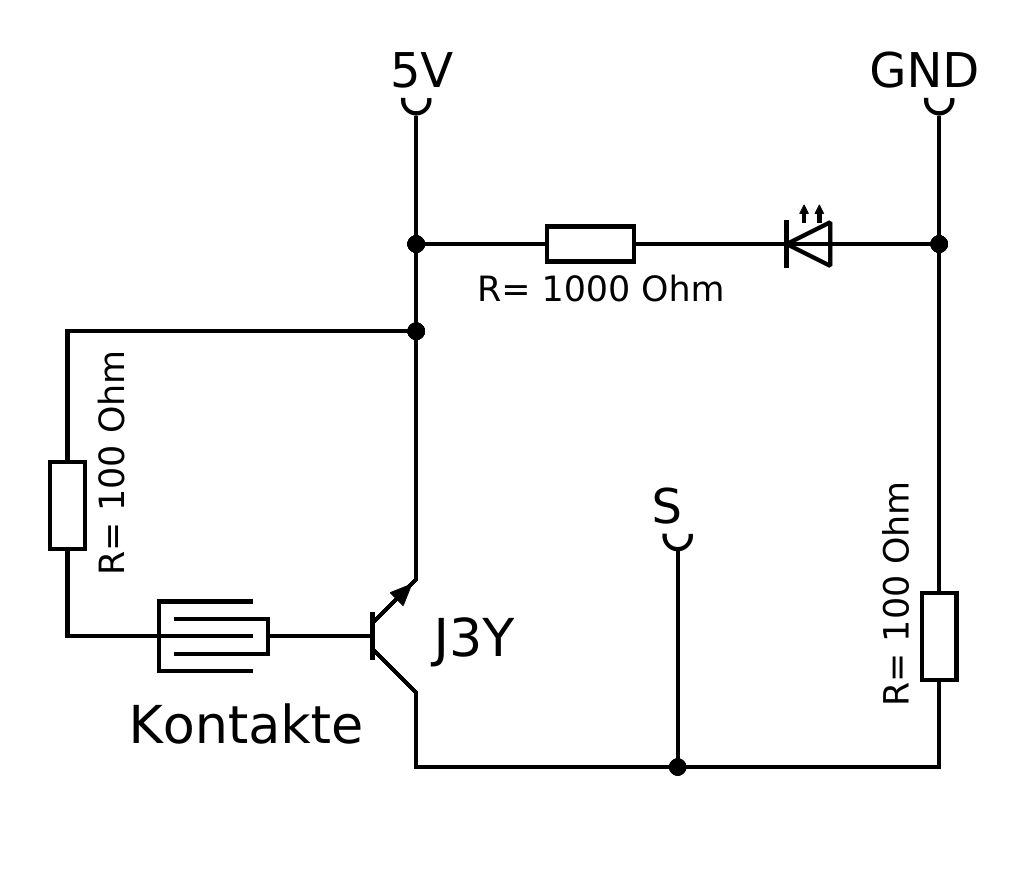
\includegraphics[width=0.5\textwidth]{./Zeichnungen/tropfensensor-ersatz.png}
	\caption{Schaltplan eines Tropfensensors.}
\end{figure}

\begin{projekt}[Automatischer Scheibenwischer]\label{proj:auto-scheibenwischer}
	Baue einen Scheibenwischer, der automatisch startet, wenn Feuchtigkeit registriert wird. Je nach Feuchtigkeitslevel soll eine von drei Geschwindigkeiten ausgewählt werden.
	
	\emph{Hinweis: Du kannst die vorkonfigurierten Blöcke von Nepo für den Tropfensensor verwenden oder einen analogen Sensor konfigurieren, dessen Analogwert du selbst in einen Prozentwert umrechnest (0 entspricht 0\,\%, 1023 entspricht 100\,\%).}
\end{projekt}

\newpage
\section{Pulssensor}\label{sec:pulssensor}

\begin{wrapfigure}{r}{0.35\textwidth}
	\centering
	\vspace{-\baselineskip}
	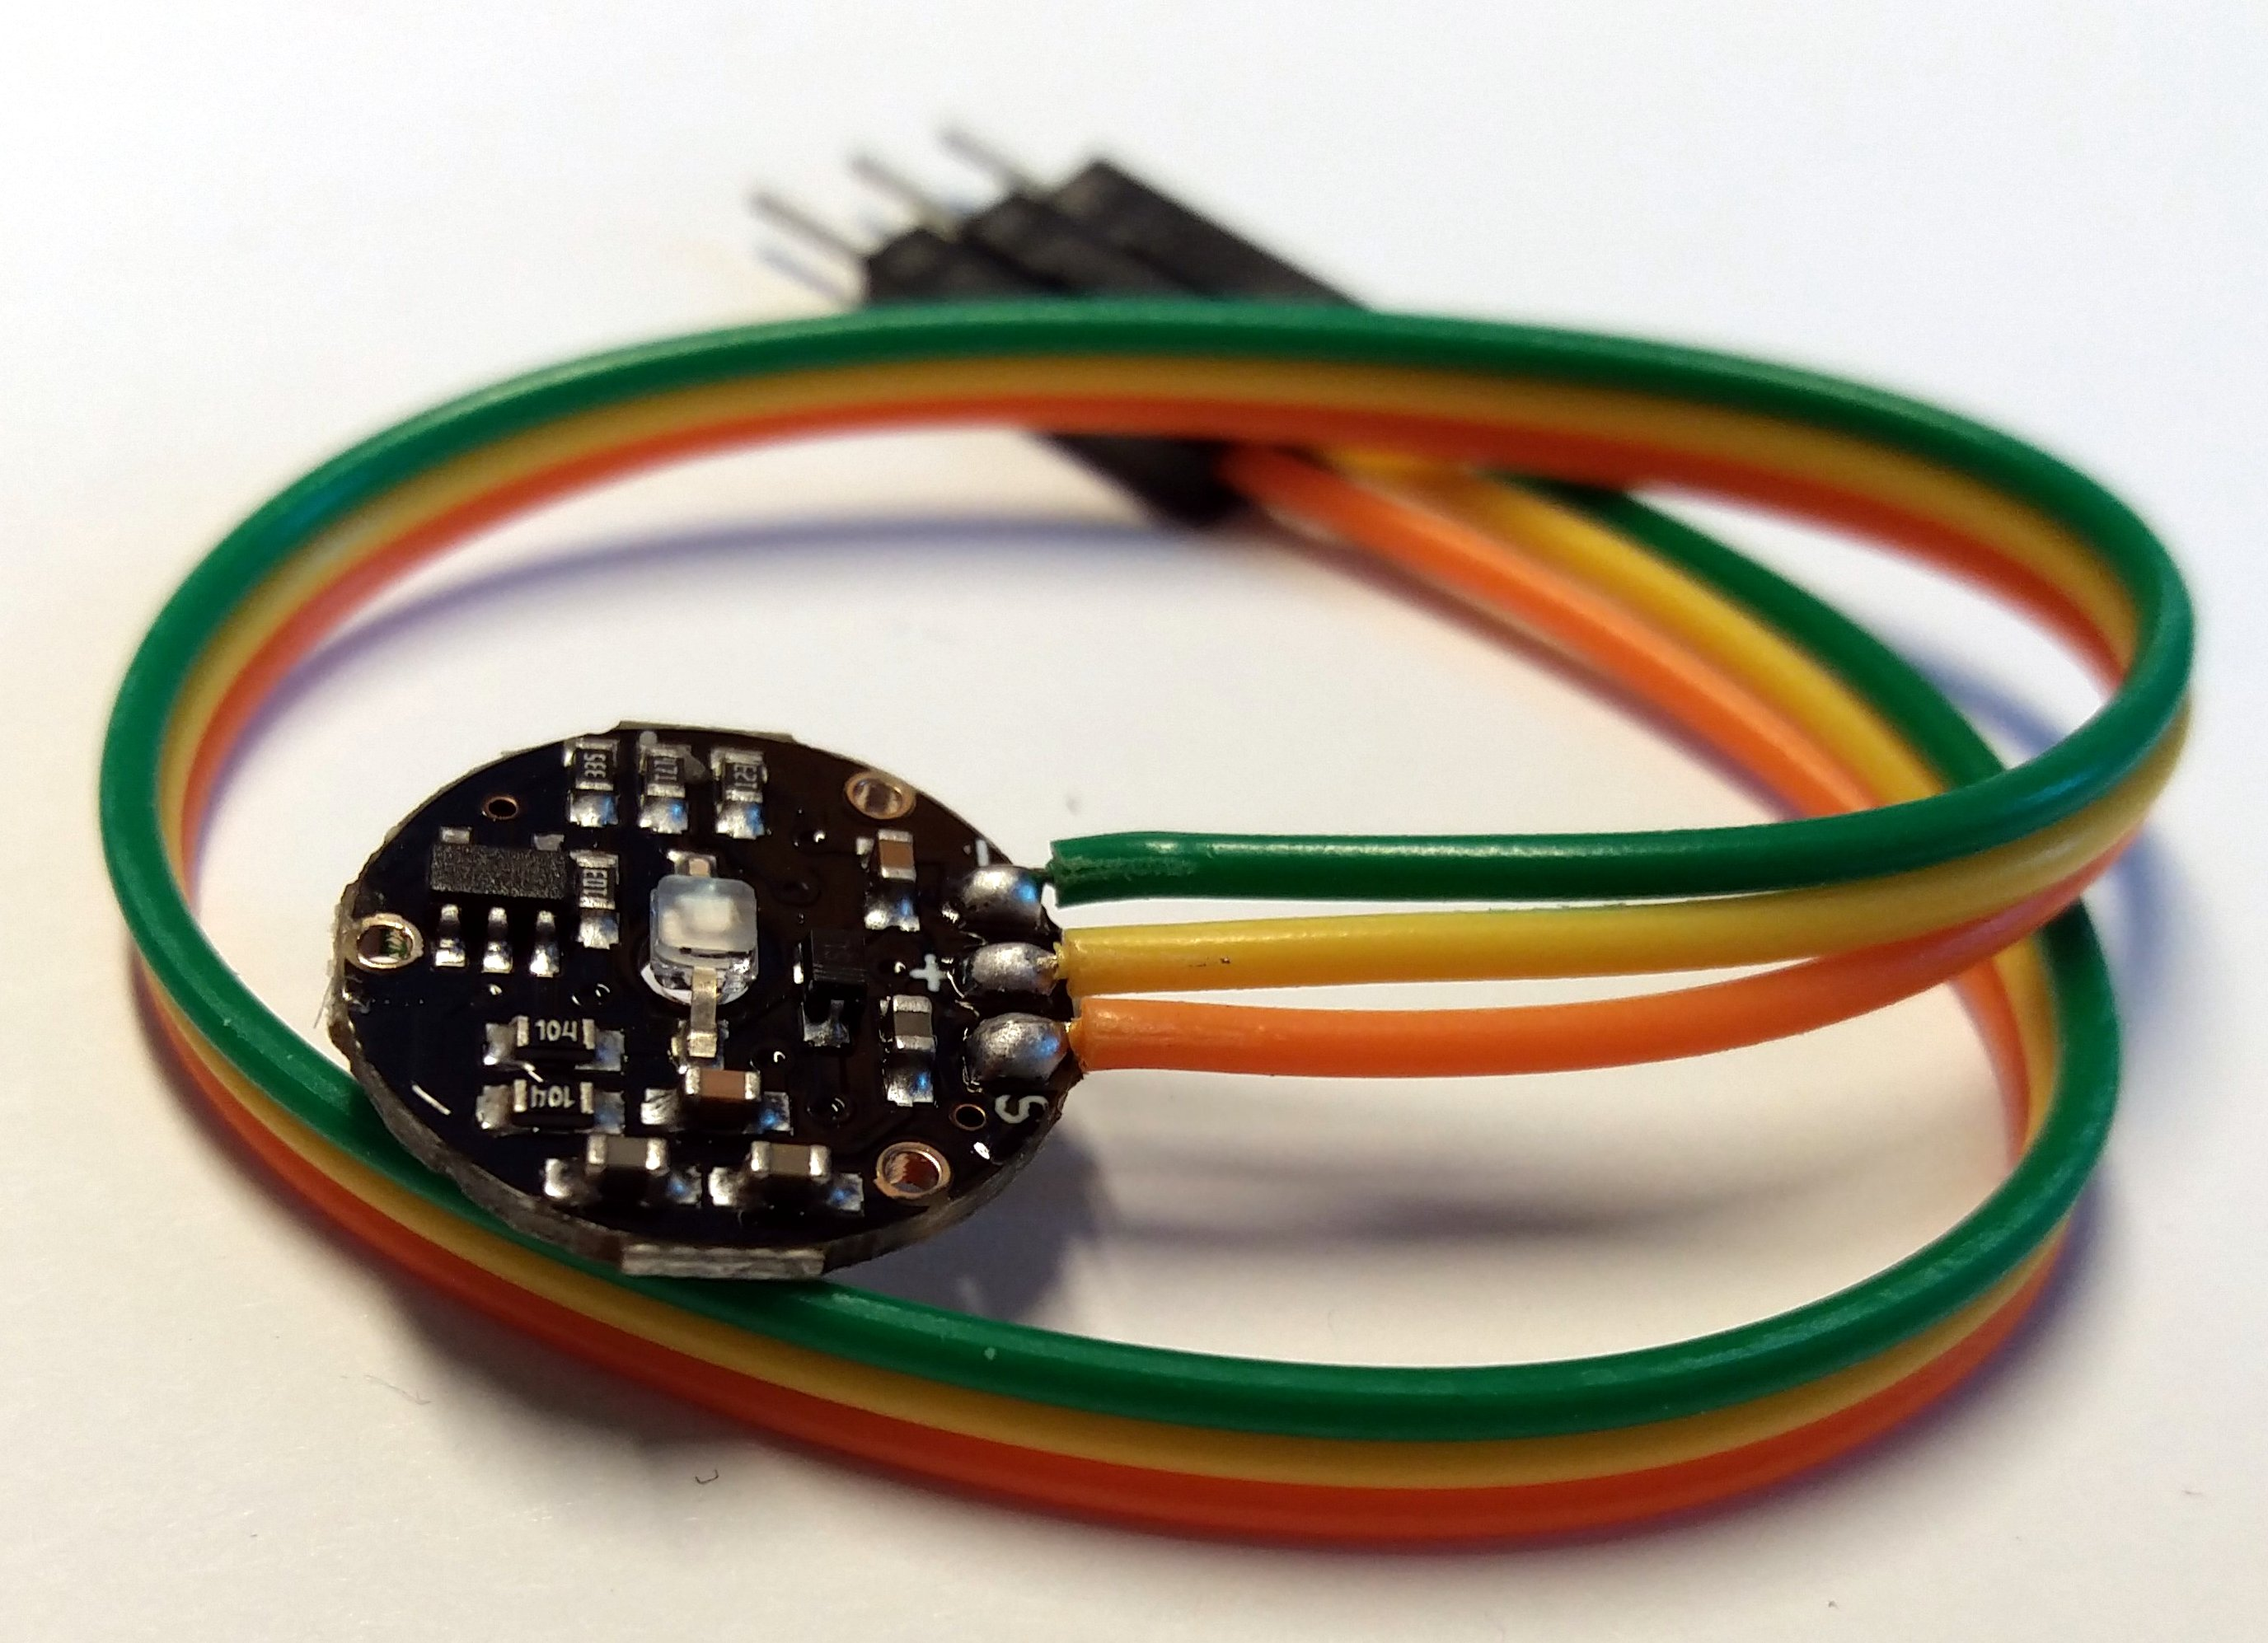
\includegraphics[width=0.3\textwidth]{./pics/pulssensor.jpg}
	\caption{Rückseite eines Pulssensors. Anschluss am Arduino: \\S > A[0-5] \qquad + > 5\,V \qquad - > GND.}
\end{wrapfigure}
Aktivitätstracker mit Pulsmessung liegen voll im Trend - aber wie funktioniert so ein Pulssensor eigentlich? Das lässt sich am einfachsten verstehen, wenn man selber einen nachbaut. Weitere Anwendungsmöglichkeiten wären übrigens Lügen-/Angstdetektoren, Schlafanalyse oder ein Alarmsystem für Risikopatienten.

Der Anschluss an den Arduino ist einfach (siehe rechts). Am Signalpin liegt eine Spannung an, die sich im Rhythmus des Herzschlags verändert und am analogen Eingang des Arduino gemessen werden kann. Dies lässt sich mit dem seriellen Plotter der Arduino IDE veranschaulichen (siehe Abb. \ref{abb:pulsmessung-serieller-plotter}). Man erkennt, dass die gemessenen Analogwerte zwischen ca. 500 und ca. 535, also in einem relativ kleinen Bereich, schwanken (35 bzw. $\SI{0,171}{\volt}$).

Als Kriterium für einen Herzschlag könnte man festlegen, dass der Analogwert über 520 liegt. Diese Werte sind jedoch wenig stabil und schwanken je nach Person und Umgebung! Man sollte unbedingt darauf achten, dass die Haut nicht verschwitzt ist und keine Bauteile auf dem Sensor berührt werden (insbesondere auf der Rückseite), damit die Ergebnisse einigermaßen zuverlässig sind. Wenn sich auf dem Arm keine brauchbaren Werte einstellen, lohnt sich ein Versuch auf dem Ringfinger oder dem Ohrläppchen.
\begin{figure}[H]
	\centering
	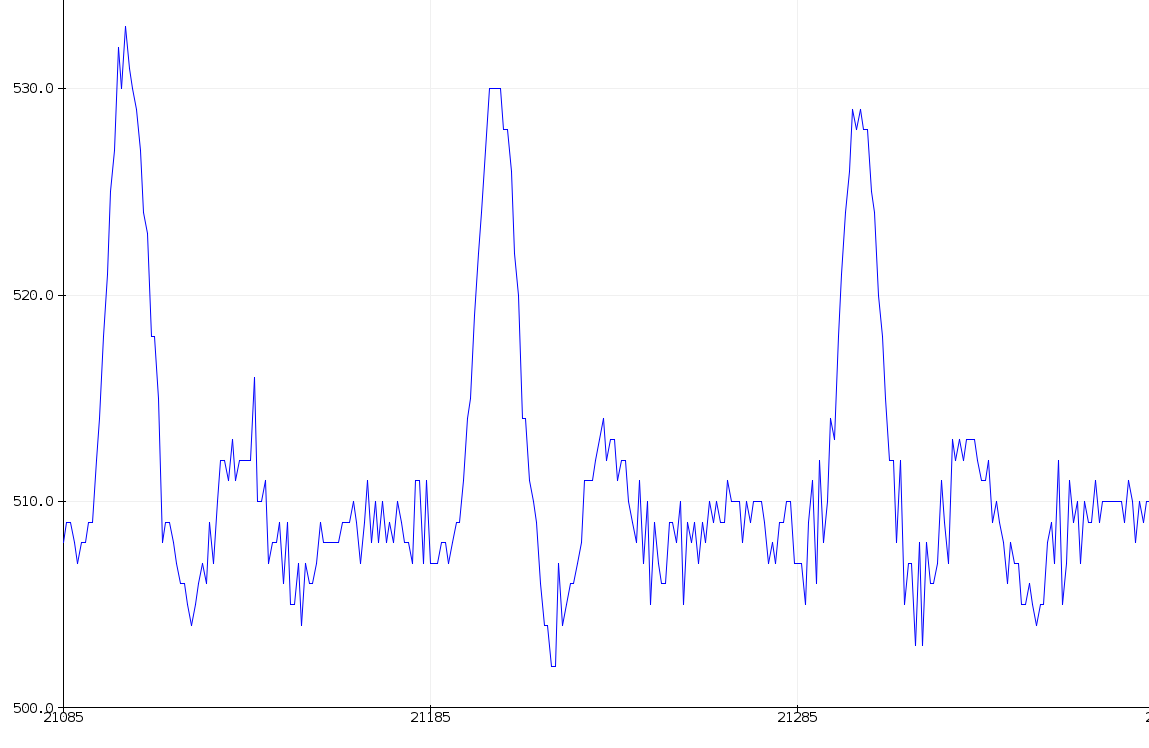
\includegraphics[width=\textwidth]{./pics/pulsmessung-serieller-plotter.png}
	\caption{Visualisierung von gemessenen Analogwerten zur Bestimmung des Pulses.}
	\label{abb:pulsmessung-serieller-plotter}
\end{figure}

Der Pulssensor kann mit den vorkonfigurierten Blöcken von Nepo oder direkt als analoger Sensor eingelesen werden. Im Hintergrund passiert das Gleiche.

% Theorie: Erkläre anhand der Bilder, wie der Sensor funktioniert
\begin{aufgabe} \emph{Theorie: Wie wird der Puls gemessen?}
	
	Für die Messung des Pulses ist die grüne LED und ein Lichtsensor zentral. Erkläre anhand der Abbildungen unten das Prinzip der optischen Pulsmessung.
\end{aufgabe}

\begin{figure}[H]
	\centering
	\begin{minipage}{0.3\textwidth}
		\centering
		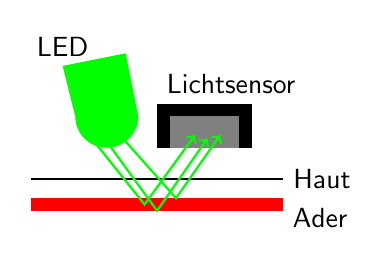
\begin{tikzpicture}[scale=0.8]
		\draw [thick] (0,0) -- (4,0) node [right] {\sffamily Haut};
		\fill [red] (0,-0.5) rectangle ++(4,0.2) node [below right] {\sffamily\color{black} Ader};
		%LED & Sensor
		\fill[green] (1.5,2) -- ++(0.2,-1) arc [start angle=0,end angle=-180,radius=0.5cm] -- ++(-0.2,0.8)  node [above] {\sffamily \color{black} LED};
		\fill [black] (2,0.5) -- ++(1.5,0) -- ++(0,0.7) -- ++(-1.5,0) node [above right] {\sffamily Lichtsensor}; 
		\fill [gray] (2.2,0.5) -- ++(1.1,0) -- ++(0,0.5) -- ++(-1.1,0);
		% Lichtstrahlen
		\draw [green, thick, ->] (1.5,0.6) -- (2.3,-0.3) -- (3,0.7);
		\draw [green, thick, ->] (1.2,0.6) -- (2,-0.5) -- (2.8, 0.65);
		\draw [green, thick, ->] (1,0.6) -- (1.8, -0.4) -- (2.6, 0.7);
		\end{tikzpicture}
	\end{minipage}
	\hfill
	\begin{minipage}{0.3\textwidth}
		\centering
		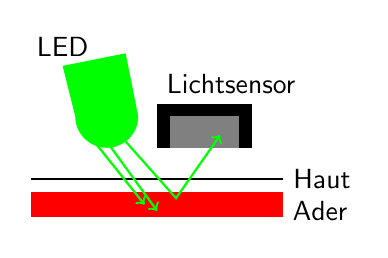
\begin{tikzpicture}[scale=0.8]
		\draw [thick] (0,0) -- (4,0) node [right] {\sffamily Haut};
		\fill [red] (0,-0.6) rectangle ++(4,0.4) node [below right] {\sffamily\color{black} Ader};
		%LED & Sensor
		\fill[green] (1.5,2) -- ++(0.2,-1) arc [start angle=0,end angle=-180,radius=0.5cm] -- ++(-0.2,0.8)  node [above] {\sffamily \color{black} LED};
		\fill [black] (2,0.5) -- ++(1.5,0) -- ++(0,0.7) -- ++(-1.5,0) node [above right] {\sffamily Lichtsensor}; 
		\fill [gray] (2.2,0.5) -- ++(1.1,0) -- ++(0,0.5) -- ++(-1.1,0);
		% Lichtstrahlen
		\draw [green, thick, ->] (1.5,0.6) -- (2.3,-0.3) -- (3,0.7);
		\draw [green, thick, ->] (1.2,0.6) -- (2,-0.5);
		\draw [green, thick, ->] (1,0.6) -- (1.8, -0.4);
		\end{tikzpicture}
	\end{minipage}
	\hfill
	\begin{minipage}{0.3\textwidth}
		\centering
		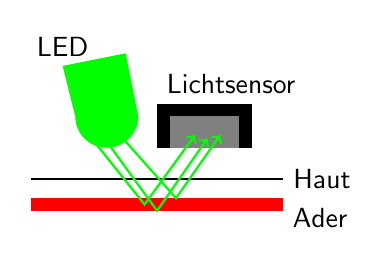
\begin{tikzpicture}[scale=0.8]
		\draw [thick] (0,0) -- (4,0) node [right] {\sffamily Haut};
		\fill [red] (0,-0.5) rectangle ++(4,0.2) node [below right] {\sffamily\color{black} Ader};
		%LED & Sensor
		\fill[green] (1.5,2) -- ++(0.2,-1) arc [start angle=0,end angle=-180,radius=0.5cm] -- ++(-0.2,0.8)  node [above] {\sffamily \color{black} LED};
		\fill [black] (2,0.5) -- ++(1.5,0) -- ++(0,0.7) -- ++(-1.5,0) node [above right] {\sffamily Lichtsensor}; 
		\fill [gray] (2.2,0.5) -- ++(1.1,0) -- ++(0,0.5) -- ++(-1.1,0);
		% Lichtstrahlen
		\draw [green, thick, ->] (1.5,0.6) -- (2.3,-0.3) -- (3,0.7);
		\draw [green, thick, ->] (1.2,0.6) -- (2,-0.5) -- (2.8, 0.65);
		\draw [green, thick, ->] (1,0.6) -- (1.8, -0.4) -- (2.6, 0.7);
		\end{tikzpicture}
	\end{minipage}
\caption{Schematische Darstellung eines Pulses und seiner optischen Vermessung.}
\end{figure}

\bigskip

% Projekt: Pulsmessung
% vorgegebenes Programm, wie man stabile Pulswerte hinbekommt?
\begin{projekt}[Pulsmesser]\label{proj:pulsmesser}
	Baue einen Pulsmesser, der anhand der Messwerte von 10 Sekunden den Puls (Herzschläge pro Minute) berechnet.
	
	\emph{Hinweis: Es kann nötig sein, sich die Werte von einem seriellen Plotter visualisieren zu lassen, um einen Eindruck vom Wertebereich und von der Grenze für die Herzschlagerkennung zu bekommen. Lasse dir ggf. von deinem Lehrer zeigen, wie man die Arduino IDE dafür einstellen muss.}
\end{projekt}

\newpage
%\newgeometry{twoside, top=1cm, outer=2.6cm, inner=2.6cm, % inner und outer sind aus irgendeinem Grund vertauscht
%	marginparwidth=2cm, marginparsep=0.3cm,% Die Breite für die Marginalien (Randbemerkungen) auf der rechten Seite
%	bottom=1cm, footskip=24pt, %Abstand zwischen Textboden und Fußzeilenboden
%	includefoot, includehead}
%\onehalfspacing
\section{Ultraschallsensor}\label{sec:ultraschallsensor}

Ultraschallsensoren ermöglichen die berührungslose Messung eines Abstands zwischen dem Sensor und dem nächstgelegenen Gegenstand. Dies macht sie zu einer interessanten Ausrüstung für Staubsaugerroboter, die nicht gegen die Wand fahren sollen, oder Einparkhilfen im Auto, die dem Fahrer anzeigen sollen, wie viel Platz er noch hat.

\begin{wrapfigure}{r}{0.35\textwidth}
	\centering
	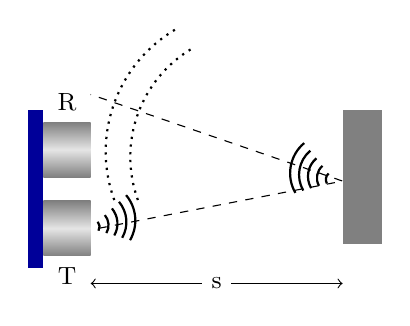
\begin{tikzpicture}
	\fill[blue!60!black] (0,0) rectangle (0.2,2);
	%Transducer
	\shade[bottom color=gray, top color=gray!20!white] (0.2,0.15) rectangle (0.8,0.5);
	\shade[bottom color=gray!20!white, top color=gray] (0.2,0.5) rectangle (0.8,0.85);
	\node at (0.5,-0.1) {\small T};
	% Receiver
	\shade[bottom color=gray, top color=gray!20!white] (0.2,1.15) rectangle (0.8,1.5);
	\shade[bottom color=gray!20!white, top color=gray] (0.2,1.5) rectangle (0.8,1.85);
	\node at (0.5,2.1) {\small R};
	% Schallwelle
	\draw [dashed] (0.9,0.5) -- (4,1.1) -- (0.8,2.2);
	\foreach \x in {1,...,5} {
		\draw [thick] (0.8+\x *0.1,0.5-\x*0.03) arc [start angle=-30, end angle=40, radius=\x mm];
		\draw [thick] (3.9-\x *0.1,1.1-\x*0.03) arc [start angle=210, end angle=130, radius=\x mm];
	}
	\draw [thick,dotted] (3.9-25*0.1,1.1-8*0.03) arc [start angle=200, end angle=120, radius=16 mm];
	\draw [thick,dotted] (3.9-28*0.1,1.1-8*0.03) arc [start angle=200, end angle=120, radius=18 mm];
	%Hindernis
	\fill[gray] (4,0.3) rectangle (4.5,2);
	% Strecke
	\draw [<->] (0.8,-0.2) -- (4,-0.2);
	\node [fill=white] at (2.4,-0.2) {\small s};
	\end{tikzpicture}
\end{wrapfigure}
Die wichtigsten Bestandteile des Ultraschallsensors sind der \enquote{Transducer} (\textbf{T}) und der \enquote{Receiver} (\textbf{R}). Der Transducer ist praktisch ein Lautsprecher, der für uns nicht hörbare Schallwellen aussendet. Der Receiver entspricht einem Mikrofon für Schallwellen. Die Schallwellen werden also vom Transducer ausgesendet, an einem Hindernis reflektiert und vom Receiver empfangen.

Der Ultraschallsensor verfügt über vier Pins. GND und VCC (5\,V) sind wie üblich zu belegen und dienen der Energieversorgung. Der Trigger-Pin dient dazu, einen Ultraschallpuls auszusenden - wird er für 10 Mikrosekunden auf ein HIGH-Potential gebracht, wird der Ultraschallpuls getriggert. Wenn dies geschieht, wird der Echo-Pin von der Elektronik des Sensors auf ein HIGH-Potential gebracht, das so lange anhält, bis der Receiver die reflektierte Schallwelle empfängt. 

\begin{wrapfigure}{r}{0.4\textwidth}
	\centering
	
\includegraphics[width=0.4\textwidth]{./pics/gibEntfernung.png}
\end{wrapfigure}
Die Zeit, die der Echo-Pin auf HIGH liegt, gibt also an, wie lange der Schall braucht, um vom Sensor zum Hindernis und zurück zu gelangen. 
%Sie kann vom Arduino mithilfe des Befehls 
%
%\button{lese Puls-Pin <\_> Timeout <\_>} gemessen werden. Der Timeout gibt dabei an, nach wie vielen Mikrosekunden der Arduino aufhört, auf eine reflektierte Schallwelle zu warten.
Mit Hilfe der Schallgeschwindigkeit wird dann berechnet, welche Strecke der Schall zurückgelegt hat. Diese Berechnungen werden praktischerweise von den vorkonfigurierten Nepo-Blöcken übernommen, sodass man direkt die Strecke erhält.

%\begin{aufgabe} \emph{Entfernungen messen}
%	
%	\begin{wrapfigure}{r}{0.48\textwidth}
%		\centering
%		\vspace{-\baselineskip}
%		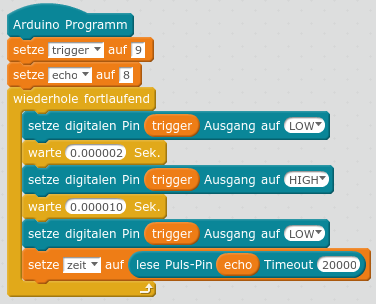
\includegraphics[width=0.48\textwidth]{./pics/ultraschallsensor-start.png}
%		\vspace{-\baselineskip}
%	\end{wrapfigure}
%	Das rechts abgebildete Programm zeigt, wie der Trigger, der mit D9 am Arduino verbunden ist, für genau 10 Mikrosekunden auf HIGH gestellt und dann der Echo-Pin, der mit D8 am Arduino verbunden ist, zur Zeitmessung verwendet wird. In der Variable \texttt{zeit} ist am Ende also die \emph{Zeit in Mikrosekunden} gespeichert, die die Schallwellen vom Sensor zum Hindernis und zurück gebraucht haben.
%	
%	Erweitere das Programm so, dass die Entfernung vom Mikrocontroller zum Hindernis berechnet und auf dem seriellen Monitor ausgegeben wird. Überprüfe deine Ultraschall-Messung mit dem Geodreieck.
%	
%	\emph{Hinweise:} 
%	\begin{itemize}[itemsep=0mm,parsep=0mm]
%		\item Schallwellen breiten sich in Luft mit Schallgeschwindigkeit aus - diese beträgt etwa $330\,\frac{\text{m}}{\text{s}}$.
%		\item $\SI{1}{\milli\second} = \SI{1000}{\micro\second}$ (Mikrosekunden)
%	\end{itemize}
%\end{aufgabe}
%\restoregeometry
%\onehalfspacing

%\begin{aufgabe} \emph{Kalibrierung}
%	
%	Die Schallgeschwindigkeit hängt auch von der Temperatur der Luft ab. Dementsprechend kann es sein, dass die mit dem Wert $330\,\frac{\text{m}}{\text{s}}$ ermittelten Entfernungen (zu) ungenau sind.
%	
%	Um einen besseren Wert der Schallgeschwindigkeit zu ermitteln, kann man die Strecke zum Hindernis mit einem Geodreieck oder Maßband genau festlegen und die Zeit, die der Schall braucht wie oben beschrieben messen. Bestimme daraus einen besseren Wert für die Schallgeschwindigkeit.
%\end{aufgabe}

\bigskip
\begin{projekt}[Einparkhilfe für ein Auto] \label{proj:einparkhilfe}
	Baue eine Einparkhilfe für ein Auto, die umso schneller piepst, je näher man dem Hindernis kommt. Ab einer Entfernung von 30\,cm soll der Ton durchgängig ertönen.
\end{projekt}

\begin{recherche}{Wie wird Ultraschall erzeugt und gemessen?}
	Die Erzeugung des Ultraschalls beruht wie beim Piezo-Summer auf dem inversen piezo-elektrischen Effekt (vgl. S. \pageref{piezo-effekt}); die Messung des Ultraschalls beruht auf dem piezo-elektrischen Effekt. Recherchiere im Internet die Hintergründe dieser Effekte und fasse sie zusammen.
\end{recherche}




\newpage
\section{RFID}\label{sec:rfid}

\begin{wrapfigure}{r}{0.4\textwidth}
	\centering
	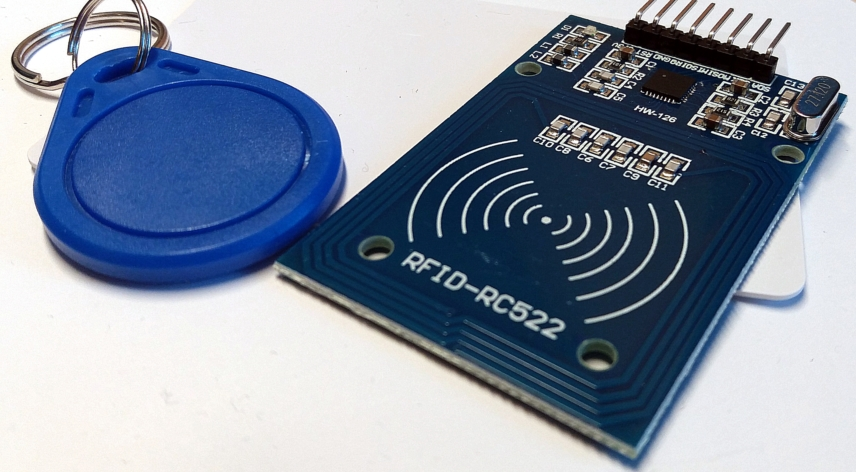
\includegraphics[width=0.35\textwidth]{./pics/rfid.jpg}
	\caption{RFID-Empfänger (rechts) mit blauem RFID-Sender (links).}
\end{wrapfigure}
Mit RFID-Chips (\emph{\textbf{r}adio \textbf{f}requency \textbf{id}entification}) lässt sich ein digitaler Schlüssel bauen, um zum Beispiel Türen abzusichern. Der RFID-Empfänger sendet über die rechteckige Spule Radiowellen, welche Energie transportieren. Diese empfängt der RFID-Sender (blauer Chip oder auch weiße Karte), woraufhin er seine eizigartige ID zurücksendet. Diese wird wiederum von der Rechteckspule empfangen und elektronisch so aufbereitet, dass man am Arduino die ID lesen kann.

\begin{wrapfigure}{r}{0.3\textwidth}
	\centering
	\vspace{-0.5\baselineskip}
	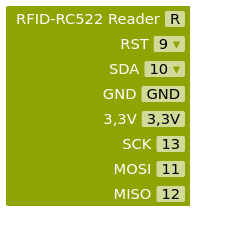
\includegraphics[width=0.28\textwidth]{./pics/rfid-konfiguration.png}
	\vspace{-0.5\baselineskip}
\end{wrapfigure}
Die Verbindung mit dem Arduino erfolgt über ein \emph{Serial Peripheral Interface (SPI)} (weitere Informationen unten), weshalb die meisten Pins festgelegt sind (siehe rechts). Der RST-Pin und der SDA-Pin lassen sich ggf. noch ändern. Wichtig: Der Mikrocontroller auf dem RFID-Chip arbeitet mit einem Logiklevel von $\SI{3,3}{\volt}$ und würde durchbrennen, wenn man ihn an 5\,V anschließt. Der Arduino verfügt direkt neben dem 5\,V-Anschluss auch über einen 3,3\,V-Anschluss. Der IRQ-Pin des RFID-Empfängers wird nicht benötigt und kann ignoriert werden.

\begin{wrapfigure}{r}{0.45\textwidth}
	\centering
	\vspace{-0.5\baselineskip}
	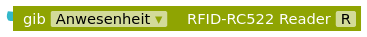
\includegraphics[width=0.45\textwidth]{./pics/rfid-gibAnwesenheit.png}
	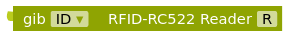
\includegraphics[width=0.35\textwidth]{./pics/rfid-gibID.png}
	\vspace{-0.5\baselineskip}
\end{wrapfigure}
Zur Programmierung kann man die bloße Anwesenheit eines RFID-Senders abfragen oder die ID eines RFID-Senders. Die Anwesenheitsabfrage unterscheidet nicht, welcher RFID-Sender anwesend ist, sie liefert also bei \emph{jedem} RFID-Sender \texttt{true} zurück. Sinnvoller ist also in den meisten Fällen die Abfrage der einzigartigen ID des RFID-Senders, um diese abspeichern und im nächsten Programm darauf reagieren zu können. Ein Beispielprogramm zeigt Abbildung \ref{abb:rfid-bsp}.

\begin{figure}[H]
	\centering
	\includegraphics[width=0.7\textwidth]{./pics/rfid-bsp.png}
	\caption{Beispielprogramm zum Auslesen eines RFID-Senders in Form einer weißen Karte.}
	\label{abb:rfid-bsp}
\end{figure}

\emph{Fehlerquellen:} Bei der Programmierung gibt es zwei Fehlerquellen zu beachten, die man möglichst vermeiden sollte:
\begin{itemize}[itemsep=0ex,parsep=0ex]
	\item Werden die Befehle \texttt{gib ID} und \texttt{gib Anwesenheit} kurz hintereinander verwendet, wird der zweite Befehl nicht funktionieren, weil dazu (durch die Implementierung im Hintergrund) immer eine neue Karte erkannt werden muss.
	\item Für den Vergleich von vorgegebener ID und eingelesener ID muss für beide eine Variable vom Typ Zeichenkette angelegt werden, damit Nepo keinen Fehler anzeigt. Das unten abgebildete Beispiel erzeugt also einen Fehler. (Hintergrund: Wenn die vorgegebene ID nicht als Zeichenkette (String) definiert wird, wird sie als sogenanntes Character-Array behandelt. Da die eingelesene ID aber vom Typ String ist, sollen sozusagen Äpfel mit Birnen verglichen werden.)
	\begin{figure}[H]
		\centering
		\includegraphics[width=0.7\textwidth]{./pics/rfid-fehler-vgl-chararray-mit-string.png}
		\caption{Der Vergleich von vorgegebener ID und eingelesener ID erzeugt hier einen Fehler.}
	\end{figure}
\end{itemize}

% Projekt: Katzentür, die nur öffnet, wenn richtige ID erkannt
\begin{projekt}[Katzentür] \label{proj:katzentuer}
	Baue und programmiere einen Prototypen für eine Katzentür, die sich automatisch öffnet, wenn die Katze (mit RFID-Chip am Halsband) sich der Tür nähert.
	
	\emph{Erweiterung:} Schließe einen weiteren RFID-Empfänger am Arduino an (siehe Informationen unten). Einer der RFID-Empfänger soll sich draußen, der andere drinnen befinden. Programmiere nun drei Modi, zwischen denen sich hin- und herschalten lässt:
	\begin{itemize}[itemsep=0ex, parsep=0ex]
		\item Standard: Tür geht immer auf,
		\item Tag: Tür geht nur von innen nach außen auf (alle Katzen sollen raus),
		\item Nacht: Tür geht nur von außen nach innen auf (alle Katzen sollen rein).
	\end{itemize}
\end{projekt}

% Info: Serial Peripheral Interface (SPI)
\begin{zsfg}{Serial Peripheral Interface (SPI)}
	
	Das \emph{Serial Peripheral Interface} (engl. für serielle periphäre Schnittstelle) ist ein Bus-System, um Daten zwischen Mikrocontrollern und integrierten Schaltkreisen nach dem Master-Slave-Prinzip auszutauschen. Der Master ist hier immer der Arduino, die Slaves sind die angeschlossenen Bauteile. Für die Kommunikation werden neben zwei Leitungen zur Spannungsversorgung (5\,V bzw. 3,3\,V und GND) vier weitere Leitungen benötigt:
	
	\begin{itemize}[itemsep=0ex, parsep=0ex]
		\item[SCLK:] \emph{Serial Clock}. Auf dieser Leitung gibt der Master den Takt an, in dem die Bits gesendet werden.
		\item[MOSI:] \emph{Master Out, Slave In}. Auf dieser Leitung sendet der Master Informationen, die die Slaves empfangen.
		\item[MISO:] \emph{Master In, Slave Out}. Auf dieser Leitung empfängt der Master Informationen, die die Slaves senden.
		\item[SS:] \emph{Slave Select}. Diese Leitung wird vom Master auf ein GND-Potential (logisch 0) gebracht, um dem damit verbundenen Slave mitzuteilen, dass die folgenden Informationen an ihn gehen sollen. Im Gegensatz zu den ersten drei Leitungen erhält jeder Slave einen eigenen SS-Pin am Master, damit dieser sie einzeln ansprechen kann (siehe Abb. XX). 
	\end{itemize}

	Da das RFID-Modul aus diesem Abschnitt auch über den I2C-Bus angesteuert werden kann, haben zwei Pins eine mehrfache Funktion. Insbesondere entspricht der SDA-Pin (im I2C-Bus die serielle Datenleitung) bei der Ansteuerung über den SPI-Bus dem SS-Pin (siehe \href{https://components101.com/wireless/rc522-rfid-module}{components101.com}).
	
	\begin{figure}[H]
		\centering
		\includegraphics[width=0.55\textwidth]{./pics/SPI-three-slaves.png}
		\caption{SPI-Verbindung mit einem Master und drei Slaves. Quelle: \href{https://de.wikipedia.org/wiki/Datei:SPI_three_slaves.svg}{Wikipedia}, Lizenz: \href{https://creativecommons.org/licenses/by-sa/3.0/deed.de}{CC-BY-SA 3.0}, \href{https://en.wikipedia.org/wiki/User:Cburnett}{Colin Burnett}.}
	\end{figure}
\end{zsfg}

%TODO: Theoretischer Hintergrudn: Schwingkreis (Recherche?)


\newpage
\section{Projektarbeit}\label{sec:projektarbeit}

\begin{ziel}
	Überlegt euch ein Arduino-Projekt, das ihr gerne umsetzen würdet, und erarbeitet euch ggf. die fehlenden Grundlagen dazu. Ihr könnt alle Bauteile aus eurem Arduino-Kit nutzen. Die Abschnitte aus diesem Kapitel geben euch eine Einführung zu einigen Bauteilen und ggf. bieten sie euch auch Ideen, was man mit dem Arduino umsetzen kann.
	
	Am Ende solltet ihr euer Projekt mit einem funktionierenden Prototypen auf einem Steckbrett vorstellen können. Zudem sollt ihr eine kurze Ausarbeitung mit folgenden Abschnitten anfertigen:
	\begin{multicols}{2}
		\begin{itemize}[parsep=0mm, itemsep=0ex]
			\item Projektziel
			\item Materialliste
			\item Schaltplan
			\item Programm (als Screenshot)
			\item Erläuterung des Schaltplans und des Programms
			\item Ausblick: Mögliche Erweiterungen oder Anwendungen
		\end{itemize}
	\end{multicols}
\end{ziel}

Mögliche übergeordnete Themen für Projekte:
\begin{itemize}
	\item Smart Home
	\item Smart Garden
	\item Verkehrsmanagement / E-Mobilität
	\item Smart Classroom
	\item \dots
\end{itemize}